\chapter{未知赛道环境中基于强化学习的端到端运动控制}
本文的第二章提出了在赛道环境已知的情况下基于模型的安全控制，然而在未知的赛道中，车辆无法依赖预先构建的环境模型进行控制决策。因此，本章将介绍一种基于强化学习的端到端运动控制方法，通过教师-学生两阶段策略学习框架，使得车辆能够在未知赛道环境中实现高效的运动控制。首先，本章介绍了问题描述与总体框架，然后详细阐述了教师策略的训练过程，包括特权信息集成与奖励函数设计，以及强化学习算法的选择和训练细节。接着，介绍了学生策略的训练过程，重点是视觉感知网络的设计和知识蒸馏方法的应用。最后，通过仿真和实车实验验证了所提方法的有效性，并进行了消融实验评估不同组件对整体性能的贡献。
\section{问题描述与总体框架}
在未知的赛道环境中，车辆需要依赖于车载传感器获取感知信息并作出运动决策。传统的基于模型的控制方法大都依赖于对环境和动力学的准确建模，而在未知环境中，这些方法的性能会大幅下降。现有的一些端到端的运动控制方法依赖2D激光雷达作为主要感知手段，但在现实世界中，激光雷达的成本较高，在某些环境条件下性能不佳（如雨雪天气），并且人类驾驶员通常仅依靠视觉信息便可实现高超的驾驶能力。因此，本章提出了一种基于强化学习的端到端运动控制方法，利用车载摄像头获取环境信息，并通过深度学习模型直接输出控制指令。

在基于视觉的竞速比赛中，车辆通过一个视角有限的前置摄像头来获取赛道信息。由于视觉信息的部分可观性，竞速任务可以被构建为一个部分可观测的马尔可夫决策过程（Partially Observable Markov Decision Process，简称POMDP）。POMDP由一个元组$(\mathcal{S}, \mathcal{A}, \Omega, \mathcal{O}, \mathcal{T}, \mathcal{R})$组成，其中
\begin{itemize}
\item $\boldsymbol{s}\in\mathcal{S}$是智能体可能的状态；
\item $\boldsymbol{u}\in\mathcal{A}$是智能体可采取的动作，包括期望加速度和前轮舵角；
\item $\boldsymbol{o}^{\dagger}\in\mathcal{O}$是智能体观测到的信息，包括深度图像和车辆自身运动状态；
\item $\mathcal{O}:\mathcal{S}\times\mathcal{A}\times\Omega\rightarrow[0,1]$是给定状态下的观测概率；
\item $\mathcal{T}:\mathcal{S}\times\mathcal{A}\times\mathcal{S}\rightarrow[0,1]$是状态转移概率，转移函数为$\boldsymbol{s}_{t+1}\sim p(\cdot\vert\boldsymbol{s}_t,\boldsymbol{u}_t)$；
\item $\mathcal{R}:\mathcal{S}\times\mathcal{A}\rightarrow\mathbb{R}, r\in\mathcal{R}$是奖励函数，用于最小化竞速时间并减少碰撞风险；
\item 智能体每一步的动作由一个基于观测信息的控制策略产生：$\boldsymbol{u}_t\sim\pi^\dagger(\cdot\vert\boldsymbol{o}^\dagger_t)$。
\end{itemize}
在这个框架下，车辆需要根据当前的视觉观测来选择最优的控制动作，以最大化累积奖励
\begin{equation}
\begin{aligned}
\mathbb{E}_{\boldsymbol{u}_t\sim\pi^\dagger(\cdot\vert\boldsymbol{o}^\dagger_t)}\left[\sum_{t=0}^{T-1}\gamma^{t}r(\boldsymbol{s}_t,\boldsymbol{u}_t)\right],
\end{aligned}
\label{equ:pomdp}
\end{equation}
其中$\gamma\in[0,1)$是折扣因子，$T$是竞速的总时间步数。

然而，强化学习在训练基于视觉的竞速控制策略时面临着诸多挑战。首先，强化学习在视觉这样的高维输入空间中通常需要大量的交互数据来学习有效的策略，这在实际环境中可能非常昂贵和耗时\cite{yarats2021improving}。其次，视觉信息的部分可观性使得学习过程更加复杂，因为智能体无法直接获取完整的环境状态，强化学习算法在训练过程中可能会遇到局部最优解、训练不稳定等问题\cite{lauri2022partially}。另外，仿真与现实之间的差距（Sim-to-Real Gap）也是一个重要的挑战，训练过程中使用的仿真环境可能无法完全捕捉现实世界中的复杂性和不确定性，导致训练得到的策略在实际环境中表现不佳\cite{tobin2017domain}。

\begin{figure}[ht]
    \centering
    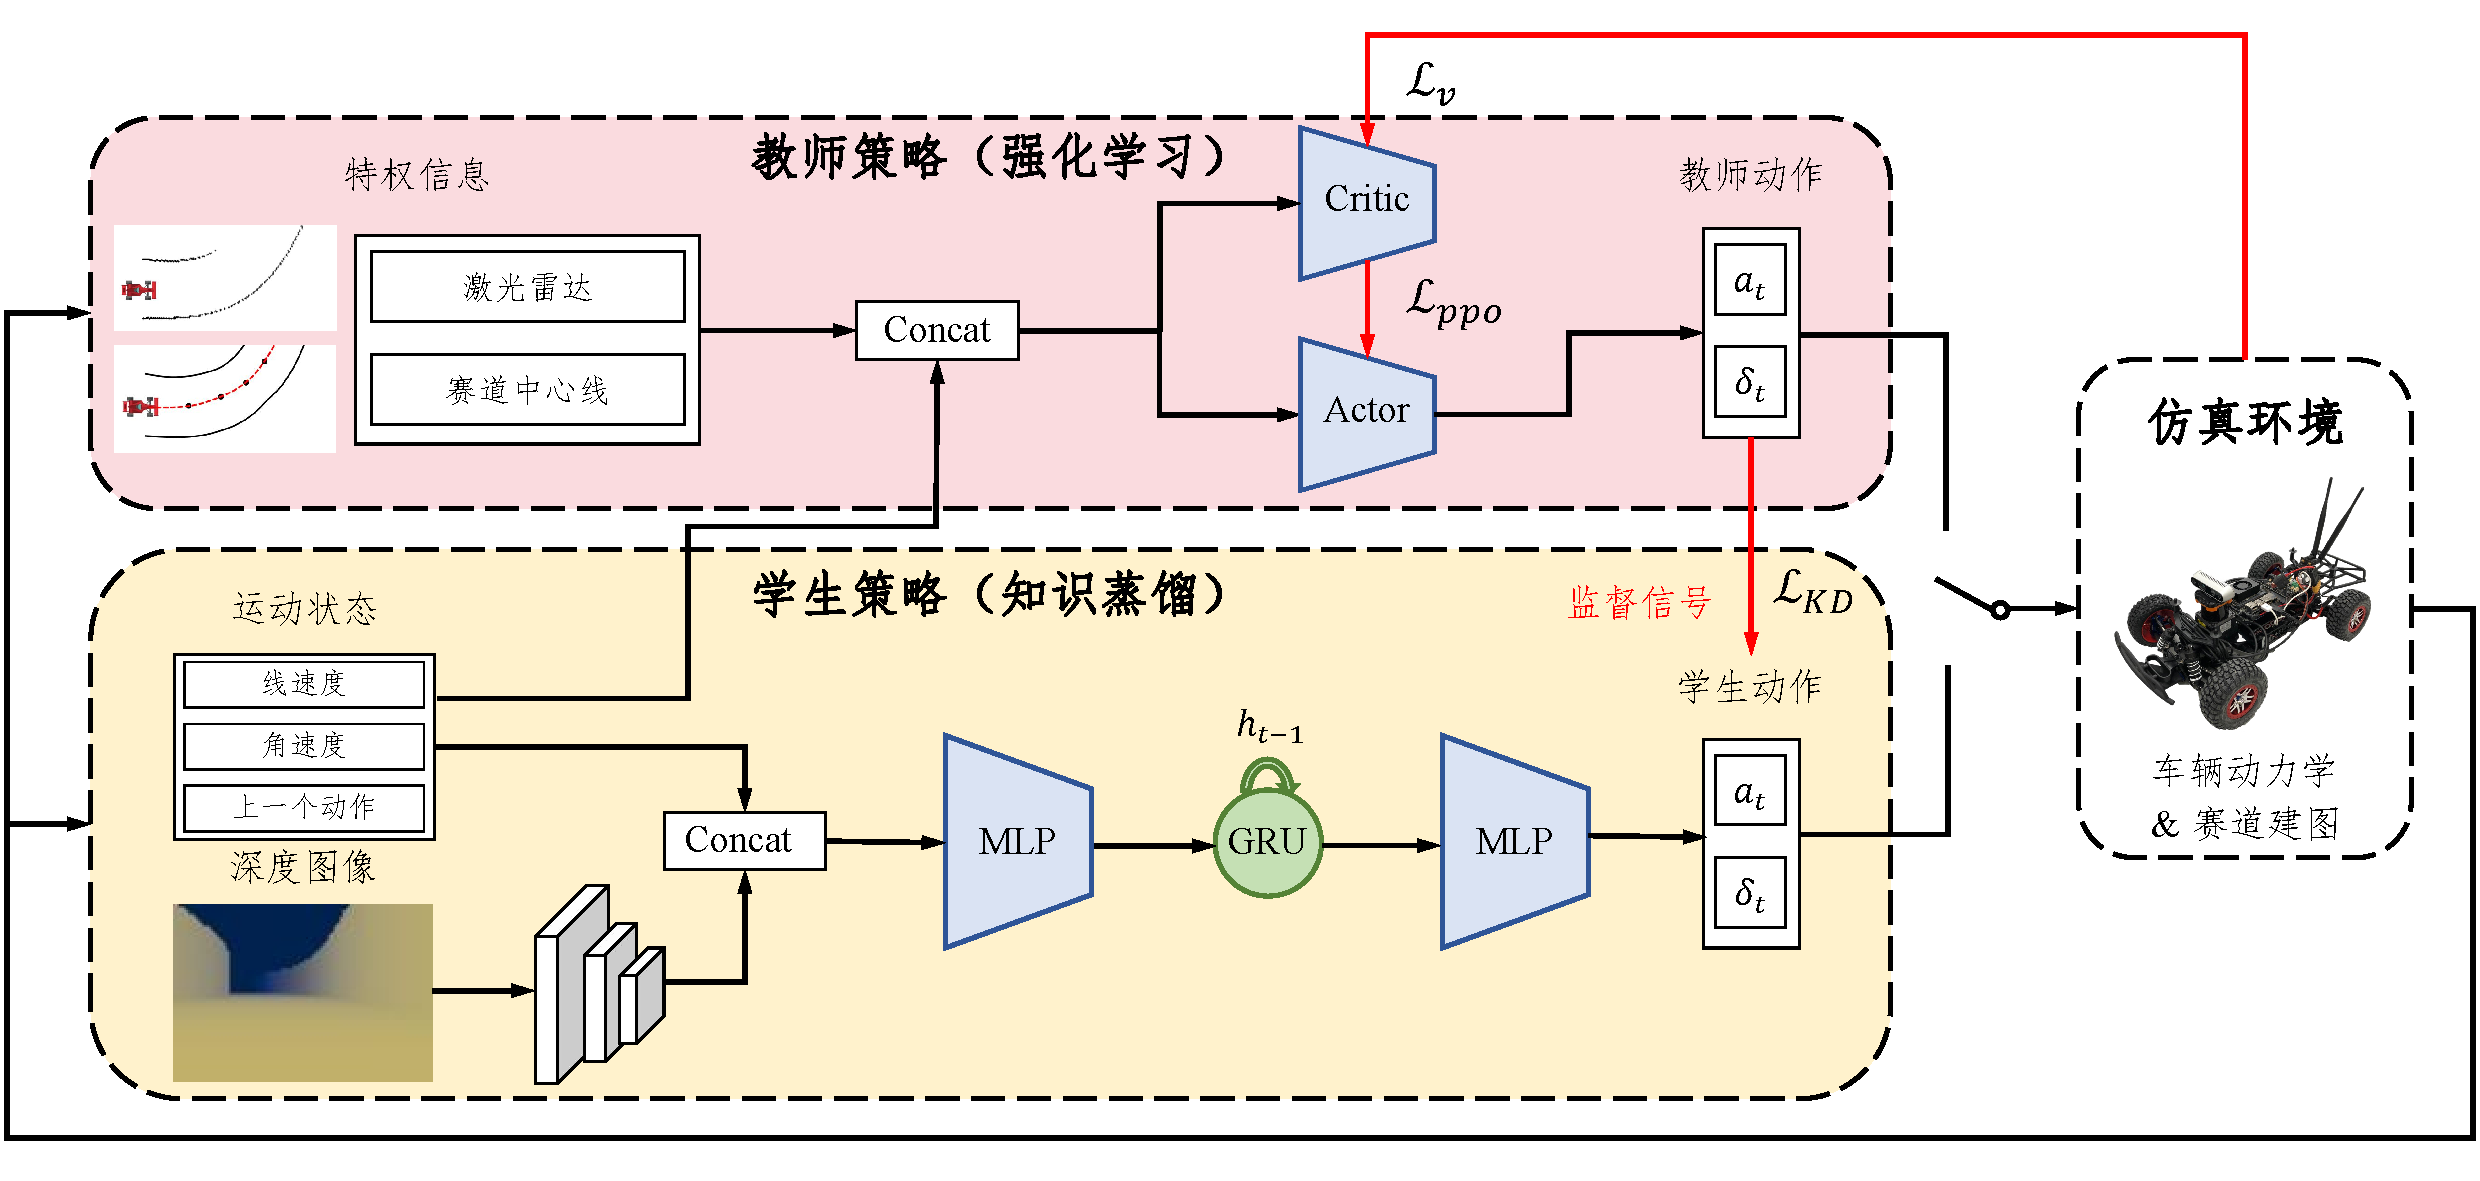
\includegraphics[width=1.0\linewidth]{figure/chapter3/two-stage.pdf}
    \caption{教师-学生两阶段策略学习框架}
    \label{fig:two-stage}
\end{figure}
为了克服这些问题，本章采用了教师-学生两阶段策略学习框架，如图\ref{fig:two-stage}所示。在第一阶段，教师策略通过强化学习算法在仿真环境中进行训练，利用低维的全局特权信息$\boldsymbol{o}_t^{\ast}$（如赛道的中心线、激光雷达扫描距离等）来加速学习过程。教师策略的目标是学习一个高性能的控制策略$\pi^\ast$，能够在仿真环境中实现快速且安全的竞速。$\pi^\ast$通过最大化累积奖励获得：
\begin{equation}
\begin{aligned}
\pi^\ast=\arg\max_{\pi^\ast}\mathbb{E}_{\boldsymbol{u}_t\sim\pi^\ast(\cdot\vert\boldsymbol{o}^\ast_t)}\left[\sum_{t=0}^{T-1}\gamma^{t}r(\boldsymbol{s}_t,\boldsymbol{u}_t)\right].
\end{aligned}
\label{equ:mdp}
\end{equation}
第二阶段，学生策略通过知识蒸馏（Knowledge Distillation，简称KD）从教师策略中学习，学生策略在训练过程中不使用任何特权信息。通过这种方式，学生策略能够在未知赛道环境中实现端到端的运动控制，同时保持较高的性能和泛化能力。学生策略通过最小化知识蒸馏损失获得：
\begin{equation}
\begin{aligned}
    \pi^\dagger=\arg\min_{\pi^\dagger}\mathcal{L}_{KD}(\pi^\ast(\cdot\vert\boldsymbol{o}^\ast_t), \pi^\dagger(\cdot\vert\boldsymbol{o}^\dagger_t)),
\end{aligned}
\label{il}
\end{equation}
其中$\mathcal{L}_{KD}$是教师策略和学生策略之间的知识蒸馏损失函数，衡量了两者输出行为之间的差异。

\section{基于强化学习的教师策略训练}
\subsection{奖励函数设计与特权信息集成}
第一阶段的教师策略的目标是通过强化学习训练一个高性能的控制策略$\pi^\ast$，能够最小化竞速时间并减少碰撞风险。然而，赛车只有在完成赛道后才能获得单圈时间的反馈，这样的稀疏奖励会导致强化学习算法训练不稳定且难以收敛\cite{andrychowicz2017hindsight}。为了解决上述问题，本文设计了一个基于特权信息的奖励函数，能够在每个时间步提供更丰富的反馈信号，从而加速学习过程。

\begin{figure}[ht]
    \centering
    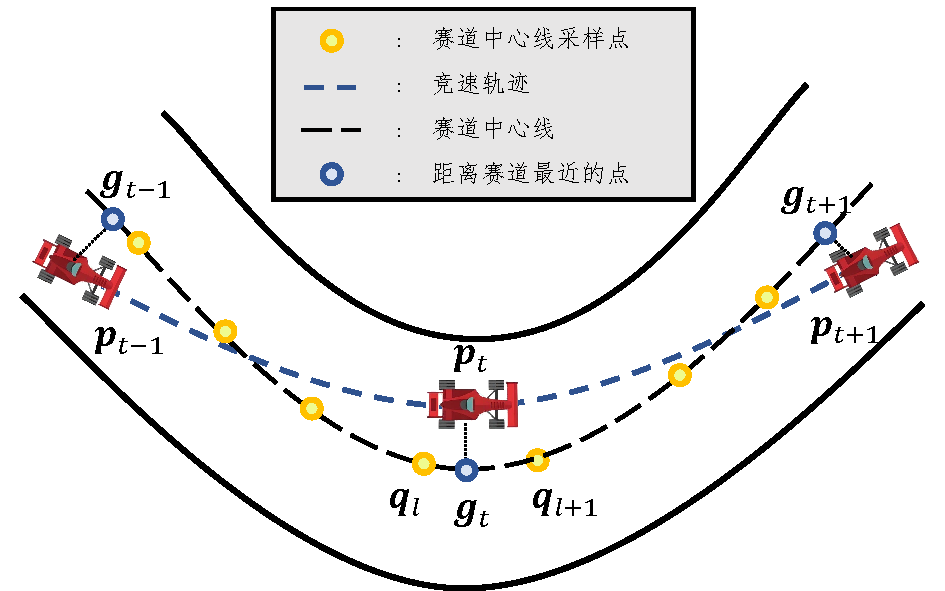
\includegraphics[width=0.7\linewidth]{figure/chapter3/reward-function.pdf}
    \caption{奖励函数设计示意图}
    \label{fig:reward-function}
\end{figure}
奖励函数引入了一个基于赛道进度的近似奖励项，鼓励赛车尽快完成赛道，如图\ref{fig:reward-function}所示；同时为了减少奖励信号的方差，折扣因子$\gamma$用于评估未来奖励，当$\gamma$足够大时，轨迹累积奖励就近似于单圈时间奖励。首先在整条赛道中心线上相隔相同距离采样了$n$个点$(\boldsymbol{q}_1,\boldsymbol{q}_2,\ldots,\boldsymbol{q}_n)$，为了在任意时刻$t$计算赛车完成赛道的进度$s_t$，我们需要计算赛车当前位置与中心线距离最近的点$\boldsymbol{g}_t$，$\boldsymbol{g}_t$位于两个中心线采样点$\boldsymbol{q}_l, \boldsymbol{q}_{l+1}$之间。这个过程可以被构建为一个优化问题：
\begin{equation}
\begin{aligned}
        \boldsymbol{g}_t, &\boldsymbol{q}_l=\mathop{\arg\min_{\boldsymbol{g}_t, \boldsymbol{q}_l}}\Vert \boldsymbol{g}_t-\boldsymbol{p}\Vert_2\\
        \text{s.t.}\quad &\boldsymbol{g}_t=\boldsymbol{q}_l+\alpha(\boldsymbol{q}_{l+1}-\boldsymbol{q}_l),\\
        &\alpha=\frac{(\boldsymbol{p}-\boldsymbol{q}_l)\cdot(\boldsymbol{q}_{l+1}-\boldsymbol{q}_l)}{\Vert \boldsymbol{q}_{l+1}-\boldsymbol{q}_l\Vert^2_2},\\
        &l\in\{1,\cdots,n-1\},\alpha\in(0,1].
\end{aligned}
\label{equ:nearest-point}
\end{equation}
因此，赛车在时刻$t$的赛道进度可以被定义为：
\begin{equation}
        s_t=s(\boldsymbol{p}_t)=\sum_{i=1}^{l-1}{\Vert \boldsymbol{q}_{i+1}-\boldsymbol{q}_i\Vert}+\Vert \boldsymbol{g}_t-\boldsymbol{q}_l\Vert.
\label{progress}
\end{equation}
赛道进度奖励项$r_{track}$可以被定义为当前赛道进度与上一个时间步的差值，即
\begin{equation}
\begin{aligned}
r_{track}=s_t-s_{t-1},
\end{aligned}
\label{equ:progress-reward}
\end{equation}
这样赛车在每个时间步都会获得一个正奖励，鼓励其尽快完成赛道。

为了防止赛车在赛道上发生碰撞，奖励函数还引入了一个碰撞惩罚项。当赛车与赛道边界发生碰撞时，奖励函数会给予负奖励，以鼓励赛车保持安全距离并减少碰撞风险。然而，常数负奖励可能导致强化学习算法训练不稳定，因为它可能会过度惩罚某些状态，导致智能体难以探索有效的策略。因此，本文设计了一个基于能量的碰撞惩罚项，当发生碰撞时，奖励函数会给予一个与速度平方成正比的负奖励，即
\begin{equation}
\begin{aligned}
r_{crash}=\begin{cases}-\lambda_{c}\Vert\boldsymbol{v}_t\Vert^2 & \text{(when collision)}\\
        0&\text{(otherwise)}\end{cases}.
\end{aligned}
\label{equ:crash-reward}
\end{equation}

另外，舵角输出的平滑性也是一个重要的考虑因素，因为过大的舵角变化可能会导致车辆失控。因此，奖励函数还包含了一个平滑性奖励项，鼓励赛车输出平滑的控制指令:
\begin{equation}
\begin{aligned}
r_{\delta}=-\lambda_{\delta}\Vert \delta_t-\delta_{t-1}\Vert.
\end{aligned}
\label{equ:smoothness-reward}
\end{equation}

综上所述，教师策略的奖励函数可以被定义为：
\begin{equation}
\begin{aligned}
r(t)=r_{track}+r_{crash}+r_{\delta},
\end{aligned}
\label{equ:reward}
\end{equation}
$\lambda_{c},\lambda_{\delta}>0$为权重系数，用于平衡不同奖励项的影响。

教师策略中引入了特权信息，在训练过程中可以提供更丰富的环境反馈，帮助强化学习算法更快地收敛到一个高性能的策略。在本文中，特权信息指的是二维激光扫描距离值和赛车前方赛道中线采样点，这些信息提供了赛道全局信息，将部分可观测环境转换为完全可观测环境，因此教师策略无需处理历史观测，只需处理马尔科夫决策问题（Markov Decision Process，简称MDP）。特权信息的集成使得教师策略能够在仿真环境中更有效地学习到如何在赛道上进行快速且安全的竞速，从而为学生策略的训练提供了一个强大的指导信号。教师策略在$t$时刻的观测为
\begin{equation}
\begin{aligned}
\boldsymbol{o}^\ast_t=[\boldsymbol{v}_t, \dot{\theta}_t, \boldsymbol{u}_{t-1}, \boldsymbol{d}_t, \boldsymbol{w}_t].
\end{aligned}
\label{equ:teacher-observation}
\end{equation}
其中$\boldsymbol{v}_t\in\mathbb{R}^2$是在车辆坐标系下的速度；$\dot{\theta}_t\in\mathbb{R}$是车辆的航向角速度；$\boldsymbol{u}_{t-1}\in\mathbb{R}^2$是上一个时间步的控制输入；$\boldsymbol{d}_t\in\mathbb{R}^{N_d}$是车辆与赛道边界的距离信息，最大距离为$d_{max}$，视场角（Field of View，简称FOV）为$\theta_{fov}$；$\boldsymbol{w}_t\in\mathbb{R}^{2N_w}$包含$N_w$个车辆前方的赛道中心线采样点，每两个点之间的距离为$\Delta d$。观测中所有的特征均进行归一化处理，以确保不同特征在训练过程中具有相似的尺度。这些特权信息能够提供关于车辆当前状态和环境的详细反馈，有助于教师策略更快地学习到有效的控制策略。另外，教师策略的动作空间为$\boldsymbol{u}_t=[a_t, \delta_t]$，其中$a_t$是期望加速度，$\delta_t$是前轮舵角，均归一化至$[-1,1]$。最大的加速度为$a_{max}$，最大的舵角为$\delta_{max}$。教师策略的网络架构如图\ref{fig:policy-architecture}所示，包含了两个全连接层，激活函数为ELU函数\cite{clevert2015fast}。
\begin{figure}[ht]
    \centering
    

\tikzset{every picture/.style={line width=0.75pt}} %set default line width to 0.75pt

\begin{tikzpicture}[x=0.75pt,y=0.75pt,yscale=-1,xscale=1]
%uncomment if require: \path (0,358); %set diagram left start at 0, and has height of 358

%Shape: Circle [id:dp5114444366440973]
\draw   (13.67,53.67) .. controls (13.67,44.46) and (21.13,37) .. (30.33,37) .. controls (39.54,37) and (47,44.46) .. (47,53.67) .. controls (47,62.87) and (39.54,70.33) .. (30.33,70.33) .. controls (21.13,70.33) and (13.67,62.87) .. (13.67,53.67) -- cycle ;
%Shape: Circle [id:dp8478206864384321]
\draw   (63.67,53.67) .. controls (63.67,44.46) and (71.13,37) .. (80.33,37) .. controls (89.54,37) and (97,44.46) .. (97,53.67) .. controls (97,62.87) and (89.54,70.33) .. (80.33,70.33) .. controls (71.13,70.33) and (63.67,62.87) .. (63.67,53.67) -- cycle ;
%Shape: Circle [id:dp009108380219839951]
\draw   (113.67,53.67) .. controls (113.67,44.46) and (121.13,37) .. (130.33,37) .. controls (139.54,37) and (147,44.46) .. (147,53.67) .. controls (147,62.87) and (139.54,70.33) .. (130.33,70.33) .. controls (121.13,70.33) and (113.67,62.87) .. (113.67,53.67) -- cycle ;
%Shape: Circle [id:dp6884441591543133]
\draw   (163.67,53.67) .. controls (163.67,44.46) and (171.13,37) .. (180.33,37) .. controls (189.54,37) and (197,44.46) .. (197,53.67) .. controls (197,62.87) and (189.54,70.33) .. (180.33,70.33) .. controls (171.13,70.33) and (163.67,62.87) .. (163.67,53.67) -- cycle ;
%Shape: Circle [id:dp7551617194224312]
\draw   (213.67,53.67) .. controls (213.67,44.46) and (221.13,37) .. (230.33,37) .. controls (239.54,37) and (247,44.46) .. (247,53.67) .. controls (247,62.87) and (239.54,70.33) .. (230.33,70.33) .. controls (221.13,70.33) and (213.67,62.87) .. (213.67,53.67) -- cycle ;
%Shape: Circle [id:dp09802310089681932]
\draw   (264,54) .. controls (264,44.8) and (271.46,37.33) .. (280.67,37.33) .. controls (289.87,37.33) and (297.33,44.8) .. (297.33,54) .. controls (297.33,63.2) and (289.87,70.67) .. (280.67,70.67) .. controls (271.46,70.67) and (264,63.2) .. (264,54) -- cycle ;
%Shape: Circle [id:dp3691489528623142]
\draw   (313.67,53.67) .. controls (313.67,44.46) and (321.13,37) .. (330.33,37) .. controls (339.54,37) and (347,44.46) .. (347,53.67) .. controls (347,62.87) and (339.54,70.33) .. (330.33,70.33) .. controls (321.13,70.33) and (313.67,62.87) .. (313.67,53.67) -- cycle ;
%Shape: Circle [id:dp809435880801653]
\draw   (363.67,53.67) .. controls (363.67,44.46) and (371.13,37) .. (380.33,37) .. controls (389.54,37) and (397,44.46) .. (397,53.67) .. controls (397,62.87) and (389.54,70.33) .. (380.33,70.33) .. controls (371.13,70.33) and (363.67,62.87) .. (363.67,53.67) -- cycle ;
%Shape: Circle [id:dp14599195508719576]
\draw   (413.67,53.67) .. controls (413.67,44.46) and (421.13,37) .. (430.33,37) .. controls (439.54,37) and (447,44.46) .. (447,53.67) .. controls (447,62.87) and (439.54,70.33) .. (430.33,70.33) .. controls (421.13,70.33) and (413.67,62.87) .. (413.67,53.67) -- cycle ;
%Shape: Circle [id:dp8091581933945314]
\draw   (463.67,53.67) .. controls (463.67,44.46) and (471.13,37) .. (480.33,37) .. controls (489.54,37) and (497,44.46) .. (497,53.67) .. controls (497,62.87) and (489.54,70.33) .. (480.33,70.33) .. controls (471.13,70.33) and (463.67,62.87) .. (463.67,53.67) -- cycle ;
%Shape: Circle [id:dp09396098090105187]
\draw   (563.67,53.67) .. controls (563.67,44.46) and (571.13,37) .. (580.33,37) .. controls (589.54,37) and (597,44.46) .. (597,53.67) .. controls (597,62.87) and (589.54,70.33) .. (580.33,70.33) .. controls (571.13,70.33) and (563.67,62.87) .. (563.67,53.67) -- cycle ;
%Shape: Circle [id:dp23851298876244642]
\draw   (613.67,53.67) .. controls (613.67,44.46) and (621.13,37) .. (630.33,37) .. controls (639.54,37) and (647,44.46) .. (647,53.67) .. controls (647,62.87) and (639.54,70.33) .. (630.33,70.33) .. controls (621.13,70.33) and (613.67,62.87) .. (613.67,53.67) -- cycle ;
%Shape: Circle [id:dp9807159177875765]
\draw   (513.67,53.67) .. controls (513.67,44.46) and (521.13,37) .. (530.33,37) .. controls (539.54,37) and (547,44.46) .. (547,53.67) .. controls (547,62.87) and (539.54,70.33) .. (530.33,70.33) .. controls (521.13,70.33) and (513.67,62.87) .. (513.67,53.67) -- cycle ;
%Straight Lines [id:da037973696127121315]
\draw    (330.1,76.71) -- (330.1,102.86) ;
\draw [shift={(330.1,104.86)}, rotate = 270] [color={rgb, 255:red, 0; green, 0; blue, 0 }  ][line width=0.75]    (10.93,-3.29) .. controls (6.95,-1.4) and (3.31,-0.3) .. (0,0) .. controls (3.31,0.3) and (6.95,1.4) .. (10.93,3.29)   ;
%Shape: Circle [id:dp46007404210398106]
\draw   (214,167) .. controls (214,157.8) and (221.46,150.33) .. (230.67,150.33) .. controls (239.87,150.33) and (247.33,157.8) .. (247.33,167) .. controls (247.33,176.2) and (239.87,183.67) .. (230.67,183.67) .. controls (221.46,183.67) and (214,176.2) .. (214,167) -- cycle ;
%Shape: Circle [id:dp8287274635139452]
\draw   (264,167) .. controls (264,157.8) and (271.46,150.33) .. (280.67,150.33) .. controls (289.87,150.33) and (297.33,157.8) .. (297.33,167) .. controls (297.33,176.2) and (289.87,183.67) .. (280.67,183.67) .. controls (271.46,183.67) and (264,176.2) .. (264,167) -- cycle ;
%Shape: Circle [id:dp02530467227910671]
\draw   (313.67,167.67) .. controls (313.67,158.46) and (321.13,151) .. (330.33,151) .. controls (339.54,151) and (347,158.46) .. (347,167.67) .. controls (347,176.87) and (339.54,184.33) .. (330.33,184.33) .. controls (321.13,184.33) and (313.67,176.87) .. (313.67,167.67) -- cycle ;
%Shape: Circle [id:dp5235317610727134]
\draw   (363.67,166.67) .. controls (363.67,157.46) and (371.13,150) .. (380.33,150) .. controls (389.54,150) and (397,157.46) .. (397,166.67) .. controls (397,175.87) and (389.54,183.33) .. (380.33,183.33) .. controls (371.13,183.33) and (363.67,175.87) .. (363.67,166.67) -- cycle ;
%Shape: Circle [id:dp23167791273539373]
\draw   (413.67,167.67) .. controls (413.67,158.46) and (421.13,151) .. (430.33,151) .. controls (439.54,151) and (447,158.46) .. (447,167.67) .. controls (447,176.87) and (439.54,184.33) .. (430.33,184.33) .. controls (421.13,184.33) and (413.67,176.87) .. (413.67,167.67) -- cycle ;
%Shape: Circle [id:dp2482346966267106]
\draw   (214,226) .. controls (214,216.8) and (221.46,209.33) .. (230.67,209.33) .. controls (239.87,209.33) and (247.33,216.8) .. (247.33,226) .. controls (247.33,235.2) and (239.87,242.67) .. (230.67,242.67) .. controls (221.46,242.67) and (214,235.2) .. (214,226) -- cycle ;
%Shape: Circle [id:dp8988810933632002]
\draw   (264,226) .. controls (264,216.8) and (271.46,209.33) .. (280.67,209.33) .. controls (289.87,209.33) and (297.33,216.8) .. (297.33,226) .. controls (297.33,235.2) and (289.87,242.67) .. (280.67,242.67) .. controls (271.46,242.67) and (264,235.2) .. (264,226) -- cycle ;
%Shape: Circle [id:dp36875494961335253]
\draw   (313.67,226.67) .. controls (313.67,217.46) and (321.13,210) .. (330.33,210) .. controls (339.54,210) and (347,217.46) .. (347,226.67) .. controls (347,235.87) and (339.54,243.33) .. (330.33,243.33) .. controls (321.13,243.33) and (313.67,235.87) .. (313.67,226.67) -- cycle ;
%Shape: Circle [id:dp700870305826061]
\draw   (363.67,225.67) .. controls (363.67,216.46) and (371.13,209) .. (380.33,209) .. controls (389.54,209) and (397,216.46) .. (397,225.67) .. controls (397,234.87) and (389.54,242.33) .. (380.33,242.33) .. controls (371.13,242.33) and (363.67,234.87) .. (363.67,225.67) -- cycle ;
%Shape: Circle [id:dp16847379044933486]
\draw   (413.67,226.67) .. controls (413.67,217.46) and (421.13,210) .. (430.33,210) .. controls (439.54,210) and (447,217.46) .. (447,226.67) .. controls (447,235.87) and (439.54,243.33) .. (430.33,243.33) .. controls (421.13,243.33) and (413.67,235.87) .. (413.67,226.67) -- cycle ;
%Straight Lines [id:da2686940665097095]
\draw    (230.67,183.67) -- (230.67,209.33) ;
%Straight Lines [id:da1629657377858197]
\draw    (230.67,183.67) -- (280.67,209.33) ;
%Straight Lines [id:da12456337363777148]
\draw    (230.67,183.67) -- (330.33,210) ;
%Straight Lines [id:da6922086464164718]
\draw    (230.67,183.67) -- (380.33,209) ;
%Straight Lines [id:da8922281365831033]
\draw    (230.67,183.67) -- (430.33,210) ;
%Straight Lines [id:da7861482750375518]
\draw    (280.67,183.67) -- (230.67,209.33) ;
%Straight Lines [id:da8981897885699681]
\draw    (280.67,183.67) -- (280.67,209.33) ;
%Straight Lines [id:da1978559698939777]
\draw    (280.67,183.67) -- (330.33,210) ;
%Straight Lines [id:da10326259777230329]
\draw    (280.67,183.67) -- (380.33,209) ;
%Straight Lines [id:da878964587383928]
\draw    (280.67,183.67) -- (430.33,210) ;
%Straight Lines [id:da12420165525697857]
\draw    (330.33,184.33) -- (230.67,209.33) ;
%Straight Lines [id:da6260438856842491]
\draw    (330.33,184.33) -- (280.67,209.33) ;
%Straight Lines [id:da9175708186681732]
\draw    (330.33,184.33) -- (330.33,210) ;
%Straight Lines [id:da22247557231055692]
\draw    (330.33,184.33) -- (380.33,209) ;
%Straight Lines [id:da7335714673331166]
\draw    (330.33,184.33) -- (430.33,210) ;
%Straight Lines [id:da6627561366748753]
\draw    (380.33,183.33) -- (230.67,209.33) ;
%Straight Lines [id:da9252760238752814]
\draw    (380.33,183.33) -- (280.67,209.33) ;
%Straight Lines [id:da7154405997935196]
\draw    (380.33,183.33) -- (330.33,210) ;
%Straight Lines [id:da5544199934534365]
\draw    (380.33,183.33) -- (380.33,209) ;
%Straight Lines [id:da201727254226859]
\draw    (380.33,183.33) -- (430.33,210) ;
%Straight Lines [id:da9847043328358758]
\draw    (430.33,184.33) -- (230.67,209.33) ;
%Straight Lines [id:da7714038757459378]
\draw    (430.33,184.33) -- (280.67,209.33) ;
%Straight Lines [id:da3703188090110988]
\draw    (430.33,184.33) -- (330.33,210) ;
%Straight Lines [id:da7936949216410111]
\draw    (430.33,184.33) -- (380.33,209) ;
%Straight Lines [id:da38887979206133705]
\draw    (430.33,184.33) -- (430.33,210) ;
%Curve Lines [id:da7359247805359732]
\draw    (471,210) .. controls (490.1,209.86) and (481.1,190.86) .. (501.1,190.86) ;
%Rounded Rect [id:dp17392944646210462]
\draw   (463.53,197.01) .. controls (463.53,190.88) and (468.5,185.91) .. (474.63,185.91) -- (531.44,185.91) .. controls (537.57,185.91) and (542.53,190.88) .. (542.53,197.01) -- (542.53,203.68) .. controls (542.53,209.8) and (537.57,214.77) .. (531.44,214.77) -- (474.63,214.77) .. controls (468.5,214.77) and (463.53,209.8) .. (463.53,203.68) -- cycle ;
%Straight Lines [id:da40773418788825355]
\draw    (330.33,122.86) -- (330.33,149) ;
\draw [shift={(330.33,151)}, rotate = 270] [color={rgb, 255:red, 0; green, 0; blue, 0 }  ][line width=0.75]    (10.93,-3.29) .. controls (6.95,-1.4) and (3.31,-0.3) .. (0,0) .. controls (3.31,0.3) and (6.95,1.4) .. (10.93,3.29)   ;
%Straight Lines [id:da616812954325922]
\draw    (330.33,250.33) -- (330.33,276.48) ;
\draw [shift={(330.33,278.48)}, rotate = 270] [color={rgb, 255:red, 0; green, 0; blue, 0 }  ][line width=0.75]    (10.93,-3.29) .. controls (6.95,-1.4) and (3.31,-0.3) .. (0,0) .. controls (3.31,0.3) and (6.95,1.4) .. (10.93,3.29)   ;
%Shape: Circle [id:dp30691063077949765]
\draw   (288.67,328.67) .. controls (288.67,319.46) and (296.13,312) .. (305.33,312) .. controls (314.54,312) and (322,319.46) .. (322,328.67) .. controls (322,337.87) and (314.54,345.33) .. (305.33,345.33) .. controls (296.13,345.33) and (288.67,337.87) .. (288.67,328.67) -- cycle ;
%Shape: Circle [id:dp46070008050395916]
\draw   (338.67,328.67) .. controls (338.67,319.46) and (346.13,312) .. (355.33,312) .. controls (364.54,312) and (372,319.46) .. (372,328.67) .. controls (372,337.87) and (364.54,345.33) .. (355.33,345.33) .. controls (346.13,345.33) and (338.67,337.87) .. (338.67,328.67) -- cycle ;

% Text Node
\draw (18,47) node [anchor=north west][inner sep=0.75pt]    {$v_{t,x}$};
% Text Node
\draw (69,47) node [anchor=north west][inner sep=0.75pt]    {$v_{t,y}$};
% Text Node
\draw (122,42.4) node [anchor=north west][inner sep=0.75pt]    {$\dot{\theta }_{t}$};
% Text Node
\draw (166,47) node [anchor=north west][inner sep=0.75pt]    {$a_{t-1}$};
% Text Node
\draw (217,44) node [anchor=north west][inner sep=0.75pt]    {$\delta _{t-1}$};
% Text Node
\draw (272,45.4) node [anchor=north west][inner sep=0.75pt]    {$d_{1}$};
% Text Node
\draw (320,49) node [anchor=north west][inner sep=0.75pt]    {$\cdots $};
% Text Node
\draw (368.13,44.4) node [anchor=north west][inner sep=0.75pt]    {$d_{N_{d}}$};
% Text Node
\draw (420.53,43.4) node [anchor=north west][inner sep=0.75pt]    {$w_{x}^{1}$};
% Text Node
\draw (470,43.4) node [anchor=north west][inner sep=0.75pt]    {$w_{y}^{1}$};
% Text Node
\draw (566.53,43.4) node [anchor=north west][inner sep=0.75pt]    {$w_{x}^{N_w}$};
% Text Node
\draw (616,43.4) node [anchor=north west][inner sep=0.75pt]    {$w_{y}^{N_w}$};
% Text Node
\draw (519,49) node [anchor=north west][inner sep=0.75pt]    {$\cdots $};
% Text Node
\draw (16,21.4) node [anchor=north west][inner sep=0.75pt]    {$\overbrace{\ \ \ \ \ \ \ \ \ \ \ \ \ \ \ \ \ \ }$};
% Text Node
\draw (40,3) node [anchor=north west][inner sep=0.75pt]   [align=left] {{\small 速度}};
% Text Node
\draw (110,4) node [anchor=north west][inner sep=0.75pt]   [align=left] {{\small 角速度}};
% Text Node
\draw (167,22.4) node [anchor=north west][inner sep=0.75pt]    {$\overbrace{\ \ \ \ \ \ \ \ \ \ \ \ \ \ \ \ \ \ }$};
% Text Node
\draw (172,4) node [anchor=north west][inner sep=0.75pt]   [align=left] {{\small 上一个动作}};
% Text Node
\draw (268,21.4) node [anchor=north west][inner sep=0.75pt]    {$\overbrace{\ \ \ \ \ \ \ \ \ \ \ \ \ \ \ \ \ \ \ \ \ \ \ \ \ \ \ \ \ }$};
% Text Node
\draw (302,4) node [anchor=north west][inner sep=0.75pt]   [align=left] {{\small 激光雷达}};
% Text Node
\draw (417,23.4) node [anchor=north west][inner sep=0.75pt]    {$\overbrace{\ \ \ \ \ \ \ \ \ \ \ \ \ \ \ \ \ \ \ \ \ \ \ \ \ \ \ \ \ \ \ \ \ \ \ \ \ \ \ \ \ \ \ \ \ \ \ \ \ \ \ \ \ }$};
% Text Node
\draw (476.05,4) node [anchor=north west][inner sep=0.75pt]   [align=left] {{\small 赛道中心线采样点}};
% Text Node
\draw (339,83) node [anchor=north west][inner sep=0.75pt]   [align=left] {{\small 逐元素}};
% Text Node
\draw (310,105) node [anchor=north west][inner sep=0.75pt]   [align=left] {{\small 归一化}};
% Text Node
\draw (320,162) node [anchor=north west][inner sep=0.75pt]    {$\cdots $};
% Text Node
\draw (320,222) node [anchor=north west][inner sep=0.75pt]    {$\cdots $};
% Text Node
\draw (505,195) node [anchor=north west][inner sep=0.75pt]   [align=left] {{\small ELU}};
% Text Node
\draw (141,186) node [anchor=north west][inner sep=0.75pt]   [align=left] {{\small 全连接层}};
% Text Node
\draw (298,322.4) node [anchor=north west][inner sep=0.75pt]    {$a_{t}$};
% Text Node
\draw (348,320.4) node [anchor=north west][inner sep=0.75pt]    {$\delta _{t}$};
% Text Node
\draw (292,297.4) node [anchor=north west][inner sep=0.75pt]    {$\overbrace{\ \ \ \ \ \ \ \ \ \ \ \ \ \ \ \ \ \ }$};
% Text Node
\draw (310,278) node [anchor=north west][inner sep=0.75pt]   [align=left] {{\small 控制量}};
% Text Node
\draw (142,208.4) node [anchor=north west][inner sep=0.75pt]    {$2\times 256$};


\end{tikzpicture}

    \caption{教师策略网络架构}
    \label{fig:policy-architecture}
\end{figure}

\subsection{强化学习算法与训练细节}
教师策略的训练采用了近端策略优化算法（Proximal Policy Optimization，简称PPO）\cite{schulman2017proximal}，这是一种基于策略梯度的方法，通过引入一个剪切函数来限制每次更新的幅度，从而提高训练的稳定性和效率。PPO算法在连续控制任务中表现出色，非常适合本章的竞速控制任务。在训练过程中，教师策略通过与仿真环境进行交互来收集数据，并使用PPO算法更新策略网络的参数。

PPO2（第二版实现）是当前应用最广泛的策略梯度强化学习算法之一，在原始PPO算法基础上进行了工程化与数值稳定性优化，属于基于策略的演员-评论家（Actor–Critic）框架\cite{konda1999actor}。其中演员网络负责根据当前状态生成动作分布，一般称为“策略网络”，训练目标为最大化轨迹的累积奖励；评论家网络则评估当前策略的状态值函数，一般称为“价值网络”，训练目标为最小化预测值与实际回报之间的误差。演员网络利用策略梯度算法\cite{sutton1999policy}来更新参数，而评论家网络则使用时序差分算法\cite{sutton1998reinforcement}来更新参数。

在策略梯度方法中，优化目标通常写为期望累计回报：$J(\theta)=\mathbb{E}_{\tau\sim p_\theta(\tau)}\left[\sum_{t=0}^{T-1}\gamma^t r_t\right]$，其中$\tau$表示一个完整的轨迹，$\theta$为演员网络$\pi^{\ast}$的参数，$p_\theta(\tau)$是由当前策略参数$\theta$定义的轨迹分布。根据策略梯度定理\cite{sutton1999policy}，策略的更新梯度可以表示为：
\begin{equation}
\begin{aligned}
\nabla_\theta J(\theta)=\mathbb{E}_{\tau\sim p_\theta(\tau)}\left[\sum_{t=0}^{T-1}\nabla_\theta \log \pi^{\ast}(\boldsymbol{u}_t|\boldsymbol{o}^{\ast}_t) A^{\pi^{\ast}}\left(\boldsymbol{o}^{\ast}_t,\boldsymbol{u}_t\right)\right],
\end{aligned}
\label{equ:policy-gradient}
\end{equation}
其中$A^{\pi^{\ast}}(\boldsymbol{o}^{\ast}_t,\boldsymbol{u}_t)$是优势函数，表示在观测$\boldsymbol{o}^{\ast}_t$下采取动作$\boldsymbol{u}_t$相对于平均水平的好处。然而，由于直接使用策略梯度方法可能会导致训练不稳定，直接沿着策略梯度更新参数可能由于步长太长，导致策略突然显著变差，进而影响训练效果。信任区域策略优化算法\cite{schulman2015trust}（Trust Region Policy Optimization，简称TRPO）通过限制策略更新的幅度来解决这个问题，从而提高训练的稳定性。TRPO算法采用重要性采样基于旧策略来估计新策略的策略梯度，并引入一个信任区域约束来限制每次更新的幅度：
\begin{equation}
\begin{aligned}
\max_\theta \quad &\mathbb{E}_{\tau\sim p_{\theta_{old}}(\tau)}\left[\frac{\pi^\ast(\boldsymbol{u}_t|\boldsymbol{o}^{\ast}_t)}{\pi^\ast_{old}(\boldsymbol{u}_t|\boldsymbol{o}^{\ast}_t)} \hat{A}_t\right],\\
\text{s.t.}\quad & \mathbb{E}_{\tau\sim p_{\theta_{old}}(\tau)}\left[D_{KL}\left(\pi^\ast_{old}(\cdot|\boldsymbol{o}^{\ast}_t), \pi^\ast(\cdot|\boldsymbol{o}^{\ast}_t)\right)\right]\leq \delta,
\end{aligned}
\label{equ:trpo}
\end{equation}
其中$D_{KL}$是（Kullback-Leibler，简称KL）散度，$\delta$是一个小的正数，表示允许的最大更新幅度，$\rho_t(\theta)=\frac{\pi^\ast(\boldsymbol{u}_t|\boldsymbol{o}^{\ast}_t)}{\pi^\ast_{old}(\boldsymbol{u}_t|\boldsymbol{o}^{\ast}_t)}$为重要性采样比率，$\hat{A}_t$是对$A^{\pi^\ast_{old}}\left(\boldsymbol{o}^{\ast}_t,\boldsymbol{u}_t\right)$的估计。然而，TRPO算法的实现较为复杂，需要求解带约束的二阶近似问题，增加了算法的计算成本。PPO2算法的关键思想是在保留原有优化问题的同时，用更简单的方式抑制$\rho_t$的过度偏离。PPO2算法直接对比率施加“软信赖域”：当更新试图使$\rho_t$超过区间$[1-\epsilon,1+\epsilon]$时，将目标增益截断，使得继续增大偏移不再带来更大目标值，从而形成如下截断目标函数：
\begin{equation}
\begin{aligned}
\mathcal{L}_{ppo}(\theta)=\mathbb{E}_{\tau\sim p_{\theta_{old}}(\tau)}\left[\min\left(\rho_t(\theta) \hat{A}_t, \text{clip}\left(\rho_t(\theta), 1-\epsilon, 1+\epsilon\right) \hat{A}_t\right)\right].
\end{aligned}
\label{equ:ppo2}
\end{equation}
该形式可由以下推导得到：对于$\hat{A}_t>0$的样本，最优更新倾向于增大$\pi^\ast(\boldsymbol{u}_t|\boldsymbol{o}^{\ast}_t)$，即增大$\rho_t$；然而若$\rho_t$远大于1，策略会过度相信旧轨迹上的动作而导致分布漂移与性能崩塌。于是使用$clip$函数将$\rho_t$上界限制在$1+\epsilon$处，则当$\rho_t>1+\epsilon$时，优化目标被固定为$(1+\epsilon)\hat{A}_t$，额外增大$\rho_t$将不再提升目标；对$\hat{A}_t<0$的样本，更新倾向于减小该动作概率（减小$\rho_t$），同理用下界$1-\epsilon$抑制过度减少。将两种符号情况统一表达即得到$\min(\cdot)$结构：其对每个时间步取未截断收益和截断收益的较小者，从而实现无需显式KL散度约束的近似信赖域更新。

为了构成完整的Actor-Critic强化学习框架，PPO2算法同时学习价值函数$V^{\ast}(o^\ast_t)$来估计优势函数$\hat{A}_t$。价值函数使用时序差分方法构建损失函数：
\begin{equation}
\begin{aligned}
\mathcal{L}_{v}(\phi)=\mathbb{E}_{\tau\sim p_{\theta_{old}}(\tau)}\left[\frac{1}{2}(r_t+\gamma V^\ast(\boldsymbol{o}^\ast_{t+1})-V^\ast(\boldsymbol{o}^\ast_t))^2\right],
\end{aligned}
\end{equation}
其中$\phi$为价值函数$V^{\ast}$的网络参数。优势函数的估计一般采用广义优势估计方法\cite{schulman2015high}（Generalized Advantage Estimation，简称GAE）。首先计算时序差分误差$\delta_t=r_t+\gamma V^\ast(\boldsymbol{o}^\ast_{t+1})-V^\ast(\boldsymbol{o}^\ast_t)$，根据时序差分思想有：
\begin{equation}
\begin{aligned}
 & A_{t}^{(1)}=\delta_{t} & & =-V^\ast(\boldsymbol{o}^\ast_t)+r_t+\gamma V^\ast(\boldsymbol{o}^\ast_{t+1}), \\
 & A_{t}^{(2)}=\delta_t+\gamma\delta_{t+1} & & =-V^\ast(\boldsymbol{o}^\ast_t)+r_t+\gamma r_{t+1}+\gamma^2V^\ast(\boldsymbol{o}^\ast_{t+2}), \\
 & A_t^{(3)}=\delta_t+\gamma\delta_{t+1}+\gamma^2\delta_{t+2} & & =-V^\ast(\boldsymbol{o}^\ast_t)+r_t+\gamma r_{t+1}+\gamma^2r_{t+2}+\gamma^3V^\ast(\boldsymbol{o}^\ast_{t+3}), \\
 & A_{t}^{(k)}=\sum_{l=0}^{k-1}\gamma^l\delta_{t+l} & & =-V^\ast(\boldsymbol{o}^\ast_t)+r_t+\gamma r_{t+1}+\ldots+\gamma^{k-1}r_{t+k-1}+\gamma^kV^\ast(\boldsymbol{o}^\ast_{t+k}).
\end{aligned}
\end{equation}
然后通过指数加权平均来平滑优势估计：
\begin{equation}
\begin{aligned}
\hat{A}_t=(1-\lambda)(A_{t}^{(1)}+\lambda A_{t}^{(2)}+\lambda^2 A_{t}^{(3)}+\ldots)=\sum_{l=0}^{\infty}(\gamma\lambda)^l \delta_{t+l},
\label{equ:gae}
\end{aligned}
\end{equation}
其中$\lambda\in[0,1]$是一个平衡偏差和方差的参数。当$\lambda=0$时，优势估计退化为单步时序差分；当$\lambda=1$时，优势估计退化为蒙特卡罗估计。通过调整$\lambda$的值，可以在训练过程中找到一个合适的平衡点，从而提高策略的学习效率和稳定性。

综合以上目标及损失函数，PPO2算法的具体流程如算法\ref{algo:ppo2}所示。教师策略的训练细节包括了批量数据大小、学习率、折扣率、优化器等超参数的设置，如表\ref{tab:PPO-hyper-param}所示。
\newpage
\renewcommand{\algorithmicrequire}{ \textbf{输入：}}
\renewcommand{\algorithmicensure}{ \textbf{输出：}}
\renewcommand{\algorithmicreturn}{ \textbf{返回：}}
\begin{algorithm}[H]
    % \begin{spacing}{3}
	\caption{PPO2算法}
	\label{algo:ppo2}
	\begin{algorithmic}[1]
    \setstretch{1.25}
        \REQUIRE 评论家网络$V^{\ast}$，演员网络$\pi^{\ast}$
		\ENSURE 最佳网络参数$\theta, \phi$
		\STATE 随机初始化网络$V^{\ast}(\boldsymbol{o}^{\ast})$和$\pi^{\ast}(\boldsymbol{o}^{\ast})$
        \STATE $\theta_{old} \leftarrow \theta, \pi^\ast_{old} \leftarrow \pi^\ast$
        \FOR{迭代次数$iter=1\rightarrow N_{iter}$}{
            \STATE 初始化经验池$\mathcal{Q}$
            \FOR{时间步$t=0\rightarrow T-1$}{
                \STATE 从环境中采样动作$\boldsymbol{u}_t\sim\pi^\ast_{old}(\cdot\vert\boldsymbol{o}^\ast_t)$
                \STATE 执行动作$\boldsymbol{u}_t$，观察奖励$r_t$和下一个观测$\boldsymbol{o}^\ast_{t+1}$
                \STATE 将$(\boldsymbol{o}^\ast_t, \boldsymbol{u}_t, r_t, \boldsymbol{o}^\ast_{t+1})$存储到经验池$\mathcal{Q}$
            }\ENDFOR
            \STATE 利用公式(\ref{equ:gae})计算广义优势函数$\hat{A}_t$
            \FOR{更新次数$j=1\rightarrow M$}{
                \STATE 从经验池$\mathcal{Q}$中随机采样N个元组$(\boldsymbol{o}^\ast_t, \boldsymbol{u}_t, r_t, \boldsymbol{o}^\ast_{t+1})_{i=1,\cdots,N}$

                \STATE 更新演员网络参数$\theta$，最大化$\mathcal{L}_{ppo}(\theta)$
                \STATE 更新评论家网络参数$\phi$，最小化$\mathcal{L}_{v}(\phi)$
            }\ENDFOR
            \STATE $\theta_{old} \leftarrow \theta, \pi^\ast_{old} \leftarrow \pi^\ast$
            }\ENDFOR
        \RETURN $\theta, \phi$
    \end{algorithmic}
    % \end{spacing}
\end{algorithm}

\begin{table}[H]
    \caption{\label{tab:PPO-hyper-param}PPO2使用的参数}
    \renewcommand{\arraystretch}{1.25}
    \begin{tabularx}{\linewidth}{X<{\centering} X<{\centering}}
        \toprule[2pt]
        参数 & 大小 \\ \midrule[1pt]
        神经网络结构（MLP） & $2\times [256, \text{ELU}]$ \\
        舵角抖动惩罚系数$\lambda_\delta$ & $0.2$ \\
        碰撞惩罚系数$\lambda_c$ & $0.3$ \\
        剪裁参数$\epsilon$ & $0.2$ \\
        广义优势估计参数$\lambda$ & $0.95$ \\
        学习率 & $3\times 10^{-4}$ \\
        批量大小 & $512$ \\
        经验池$\mathcal{Q}$的大小 & $10240$ \\
        折扣率$\gamma$ & $0.99$ \\
        优化器 & Adam \\
        控制频率 & $30Hz$ \\
        最大回合步数 & $600$ \\ \bottomrule[2pt]
    \end{tabularx}
\end{table}

\section{基于知识蒸馏的学生策略训练}
\subsection{视觉感知网络设计}
学生策略无法获得教师策略中使用的特权信息，因此需要依赖于车载摄像头获取的视觉信息来进行运动控制决策。学生策略的观测为：
\begin{equation}
\begin{aligned}
\boldsymbol{o}^\dagger_t=[\boldsymbol{I}_t, \boldsymbol{v}_t, \dot{\theta}_t, \boldsymbol{u}_{t-1}],
\end{aligned}
\label{equ:student-observation}
\end{equation}其中$\boldsymbol{I}_t\in\mathbb{R}^{H\times W}$是车辆前置摄像头捕获的深度图像，$H$、$W$分别表示图像的高度、宽度；$\boldsymbol{v}_t\in\mathbb{R}^2$是在车辆坐标系下的速度；$\dot{\theta}_t\in\mathbb{R}$是车辆的航向角速度；$\boldsymbol{u}_{t-1}\in\mathbb{R}^2$是上一个时间步的控制输入。由于学生策略只有视场角有限的深度图像作为对环境的观测，是部分可观测的，因此学生策略需要通过历史观测来推断当前环境状态，从而做出合理的控制决策。为了从视觉输入中提取有用的环境特征，学生策略设计了一个CNN-GRU-MLP的视觉感知网络，如图\ref{fig:two-stage}所示。该网络首先使用一个卷积神经网络（Convolutional Neural Network，简称CNN）$q_\psi$作为图像编码器来处理深度图像输入，提取低维空间特征$\boldsymbol{z}_t\in\mathbb{R}^{N_z}$；$\boldsymbol{z}_t$和赛车运动状态$\boldsymbol{l}_t=[\boldsymbol{v}_t, \dot{\theta}_t, \boldsymbol{u}_{t-1}]$一起被送入一个多层感知机（Multilayer Perceptron，简称MLP）$p_1$中进行特征融合，输出向量$\boldsymbol{\beta}_t\in\mathbb{R}^{N_\beta}$；然后使用一个门控循环单元（Gated Recurrent Unit，简称GRU）\cite{chung2014empirical}$p_{GRU}$来处理时间序列数据，捕捉环境的动态变化，其中循环状态$\boldsymbol{h}_t\in\mathbb{R}^{N_h}$；最后通过一个多层感知机$p_2$将循环状态$\boldsymbol{h}_t$映射到控制指令输出。网络结构可被写为：
\begin{equation}
\begin{aligned}
    &\text{图像编码器：} & & \boldsymbol{z}_t\sim q_{\psi}(\boldsymbol{I}_t),\\
    &\text{特征融合层：} & & \boldsymbol{\beta}_t=p_1(\boldsymbol{z}_t,\boldsymbol{l}_t),\\
    &\text{时序记忆层：} & & \boldsymbol{h}_{t}=p_{GRU}(\boldsymbol{\beta}_t,\boldsymbol{h}_{t-1}),\\
    &\text{控制策略层：} & &\boldsymbol{u}_t=p_2(\boldsymbol{h}_t).
\end{aligned}
\label{equ:student-net}
\end{equation}
本设计的关键在于如何有效地从视觉输入中提取环境特征，并将其与车辆运动状态进行融合，以便学生策略能够在未知赛道环境中做出合理的控制决策。CNN部分负责从深度图像中提取空间特征，GRU部分则负责捕捉时间序列中的动态变化，这种结构使得学生策略能够更好地理解环境的时空特性，从而提高控制性能。

\begin{figure}[t]
    \centering
    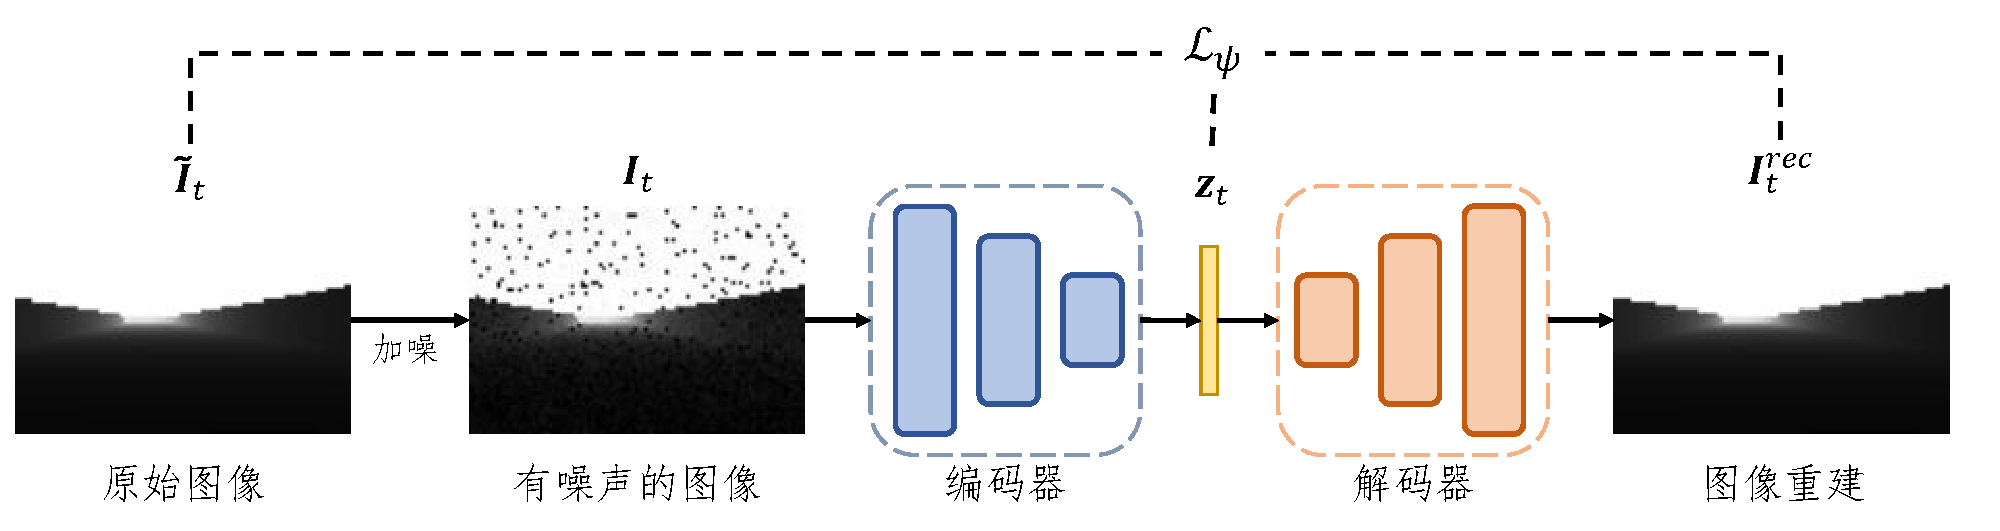
\includegraphics[width=1.0\linewidth]{figure/chapter3/vae.pdf}
    \caption{预训练的变分自编码器架构}
    \label{fig:vae-architecture}
\end{figure}
\begin{table}[t]
    \caption{\label{tab:vae-hyper-param}VAE预训练使用的参数}
    \renewcommand{\arraystretch}{1.25}
    \begin{tabularx}{\linewidth}{X<{\centering} X<{\centering}}
        \toprule[2pt]
        参数 & 大小 \\ \midrule[1pt]
        潜在空间维度$N_z$ & $64$ \\
        KL散度权重$\lambda_{KL}$ & $0.001$ \\
        学习率 & $3\times 10^{-4}$ \\
        批量大小 & $128$ \\
        经验池$\mathcal{B}$的大小 & $80000$ \\
        优化器 & Adam \\\bottomrule[2pt]
    \end{tabularx}
\end{table}
为了有效提取深度图像中的空间信息，并使学生策略能够对图像中的噪声更鲁棒，我们在训练学生策略之前预训练了一个变分自编码器（Variational Autoencoder，简称VAE）\cite{doersch2016tutorial}作为图像编码器$q_\psi$。VAE是一种生成模型，通过学习一个潜在空间来表示输入数据的分布，从而能够有效地提取输入数据的特征。预训练的VAE架构如图\ref{fig:vae-architecture}所示，包含了一个三层的卷积编码器和一个三层的卷积解码器，编码器将输入的有噪声的深度图像映射到一个低维的潜在空间$\boldsymbol{z}_t$，而解码器则从潜在空间重建出原始图像。我们的数据集从仿真中获取，通过给原始数据加噪声的方式增加编码器的鲁棒性。通过最小化重建误差和潜在空间分布之间的KL散度，VAE能够学习到一个有效的图像表示，这些表示可以还原加噪声之前的原始图像，对噪声不敏感，方便后续从仿真迁移到实物系统。VAE预训练的损失函数可以被写为：
\begin{equation}
\begin{aligned}
\mathcal{L}_{\psi}=  \mathbb{E}_{(\boldsymbol{I}_t,\tilde{\boldsymbol{I}}_t)\sim\mathcal{B}}\left[\Vert\tilde{\boldsymbol{I}}_t-\boldsymbol{I}_t^{rec}\Vert_2^2\right]+\lambda_{KL}D_{KL}(q_{\psi}(\cdot\mid\boldsymbol{I}_t)\Vert p(\boldsymbol{z}_t)),
\end{aligned}
\label{equ:vae-loss}
\end{equation}
其中$\tilde{\boldsymbol{I}}_t$是原始图像，$\boldsymbol{I}_t$是加噪声后的图像，$\mathcal{B}$是数据集，$\boldsymbol{I}_t^{rec}$是解码器重建的图像，$\lambda_{KL}$是权重系数，$p(\boldsymbol{z}_t)$是潜在空间的先验分布，通常为标准正态分布。数据集中的原始图像和加噪声后的图像均在仿真器中采集。VAE的预训练参数如表\ref{tab:vae-hyper-param}所示。

\subsection{知识蒸馏方法与训练细节}
既然教师策略可以在仿真中依赖特权信息输出高性能的控制指令，那么教师策略的输出可以作为学生策略的监督信号，指导学生策略学习如何在没有特权信息的情况下做出合理的控制决策。知识蒸馏是一种模型压缩技术，通过最小化教师策略和学生策略之间的输出差异来训练学生策略。知识蒸馏技术本质上是监督学习，在本章中，我们使用均方误差（Mean Squared Error，简称MSE）作为知识蒸馏的损失函数，定义如下：
\begin{equation}
\mathcal{L}_{KD}=\mathbb{E}_{(\boldsymbol{o}^\ast_t,\boldsymbol{o}^\dagger_t, \pi^\ast(\boldsymbol{o}^\ast_t))\sim\mathcal{D}}\left[\Vert\pi^\ast(\boldsymbol{o}^\ast_t)-\pi^\dagger(\boldsymbol{o}^\dagger_t)\Vert_2^2\right],
\label{equ:imitation-loss}
\end{equation}其中$\mathcal{D}$是从仿真环境中收集的训练数据集，包含了教师策略的观测、学生策略的观测以及教师策略的输出。通过最小化$\mathcal{L}_{KD}$，学生策略能够学习到教师策略在不同环境状态下的控制行为，从而在未知赛道环境中实现端到端的运动控制。

在训练过程中，我们使用了模仿学习中的数据集聚合（Dataset Aggregation，简称DAgger）\cite{ross2011reduction}方法来收集训练数据。DAgger方法是一种在线模仿学习算法，使用学生策略与环境进行交互来收集数据，并不断地从教师策略中获取监督信号，从而更新学生策略的参数。通过这种方式，训练出的学生策略能够更好地适应环境中的变化，并且在未知赛道环境中具有更好的泛化能力。DAgger算法的参数如表\ref{tab:kd-hyper-param}所示，具体流程如算法\ref{algo:dagger}所示。
\begin{table}[ht]
    \caption{\label{tab:kd-hyper-param}知识蒸馏使用的参数}
    \renewcommand{\arraystretch}{1.25}
    \begin{tabularx}{\linewidth}{X<{\centering} X<{\centering}}
        \toprule[2pt]
        参数 & 大小 \\ \midrule[1pt]
        特征融合层维度$N_\beta$ & $64$ \\
        循环状态维度$N_h$ & $256$ \\
        数据集$\mathcal{D}$的大小 & $2048$ \\
        学习率 & $3\times 10^{-4}$ \\
        批量大小 & $64$ \\
        学生策略的轨迹长度 & $128$ \\
        优化器 & Adam \\\bottomrule[2pt]
    \end{tabularx}
\end{table}
\begin{algorithm}[H]
    \begin{spacing}{1.25}
	\caption{DAgger算法}
    \renewcommand{\arraystretch}{1.25}
	\label{algo:dagger}
	\begin{algorithmic}[1]
        \REQUIRE 教师策略$\pi^\ast$，迭代次数$T$，混合策略权重衰减率$p\in(0,1)$
		\ENSURE 学生策略$\pi^\dagger$
        \STATE 初始化数据集$\mathcal{D}$和学生策略$\pi^\dagger$
		\FOR{$i=1, 2, \cdots, T$}{
            \STATE 计算教师策略权重$\beta_i=p^{i-1}$
            \STATE 设置混合策略$\pi_i = \beta_i\pi^\ast+(1-\beta_i)\pi^\dagger$
            \STATE 让$\pi_i$与环境交互得到一条新的轨迹$tr$
            \STATE 向$\pi^\ast$咨询示例动作得到新的数据集$\mathcal{D}_i \leftarrow \left\{ {(\boldsymbol{o}^\ast_t,\boldsymbol{o}^\dagger_t, \pi^\ast(\boldsymbol{o}^\ast_t)):(\boldsymbol{o}^\ast_t,\boldsymbol{o}^\dagger_t)\in tr}\right\}$
            \STATE 增广数据集$\mathcal{D}\leftarrow\mathcal{D}\bigcup \mathcal{D}_i$
            \STATE 在增广后的数据集上使用公式（\ref{equ:imitation-loss}）训练学生策略$\pi^\dagger$
        }
        \ENDFOR
        \RETURN 策略$\pi^\dagger$
	\end{algorithmic}
    \end{spacing}
\end{algorithm}

\subsection{仿真与域随机化技术}
为了提高学生策略的泛化能力，使其能够适应现实的赛道环境，我们在训练过程中引入了域随机化技术。域随机化是一种数据增强方法，通过在训练过程中随机改变环境的某些属性来增加训练数据的多样性，从而使模型能够更好地适应现实世界中的变化\cite{tobin2017domain, peng2018sim}。在基于视觉的赛车竞速问题中，仿真与现实的差距主要体现在车辆动力学和感知两个层面。

\textbf{车辆动力学：}首先，仿真环境使用标准的单车模型\cite{liniger2015optimization}来模拟车辆的运动行为，然后使用四阶龙格-库塔方法前向积分运算。单车模型的动力学参数使用现实世界中的数据进行标定，以确保仿真环境能够真实地反映车辆的运动特性。为了增加训练数据的多样性，我们在训练过程中对车辆动力学参数进行随机化，包括车辆的质量、转动惯量、摩擦系数、轮胎侧偏刚度、执行器延迟以及加速度和转向误差等，如表\ref{tab:domain-randomization}所示。其中$\mathcal{U}(a,b)$表示在区间$[a,b]$上均匀分布的随机变量，$\mathcal{N}(\mu,\sigma^2)$表示均值为$\mu$、方差为$\sigma^2$的正态分布随机变量。在仿真中，最大的加速度为$a_{max}=8m/s^2$，最大的舵角为$\delta_{max}=0.4rad$，最大速度为$v_{max}=8m/s$。

\begin{table}[t]
    \caption{\label{tab:domain-randomization}域随机化使用的参数}
    \renewcommand{\arraystretch}{1.25}
    \setlength{\tabcolsep}{30pt}{
    \begin{tabular}{c|ccc}
    \toprule[2pt]
    & 参数 & 单位 & 随机化 \\
    \midrule[1pt]
        \multirow{9}{*}{\rotatebox[origin=c]{90}{动力学参数}} & 车辆的质量 & $[kg]$& $\mathcal{U}(3.90, 3.95)$\\
        ~ & 车辆的转动惯量 & $[kg\cdot m^2]$& $\mathcal{U}(0.046, 0.048)$\\
        ~ & 摩擦系数 & $[-]$& $\mathcal{U}(0.7, 0.9)$\\
        ~ & 前轮侧偏刚度 & $[-]$ & $\mathcal{U}(4.5, 4.7)$ \\
        ~ & 后轮侧偏刚度 & $[-]$ & $\mathcal{U}(5.3, 5.5)$ \\
        ~ & 执行器延迟 & $[s]$ & $\mathcal{U}(0.005, 0.01)$ \\
        ~ & 加速度误差 & $[m/s^2]$ & $\mathcal{N}(0.0, 0.1^2)$ \\
        ~ & 转向误差 & $[rad]$ & $\mathcal{N}(0.0, 0.02^2)$ \\
    \midrule[1pt]
    & 参数 & 单位 & 随机化 \\
    \midrule[1pt]
        \multirow{4}{*}{\rotatebox[origin=c]{90}{感知参数}} & 雷达扫描误差 & $[m]$& $\mathcal{N}(0.0, 0.01^2)$\\
        ~ & 深度图像误差 & $[m]$& $\mathcal{N}(0.0, 0.04^2)$\\
        ~ & 线速度误差 & $[m/s]$& $\mathcal{N}(0.0, 0.1^2)$\\
        ~ & 角速度误差 & $[rad/s]$& $\mathcal{N}(0.0, 0.2^2)$\\ \bottomrule[2pt]
    \end{tabular}}
\end{table}
\begin{figure}[t]
    \centering
    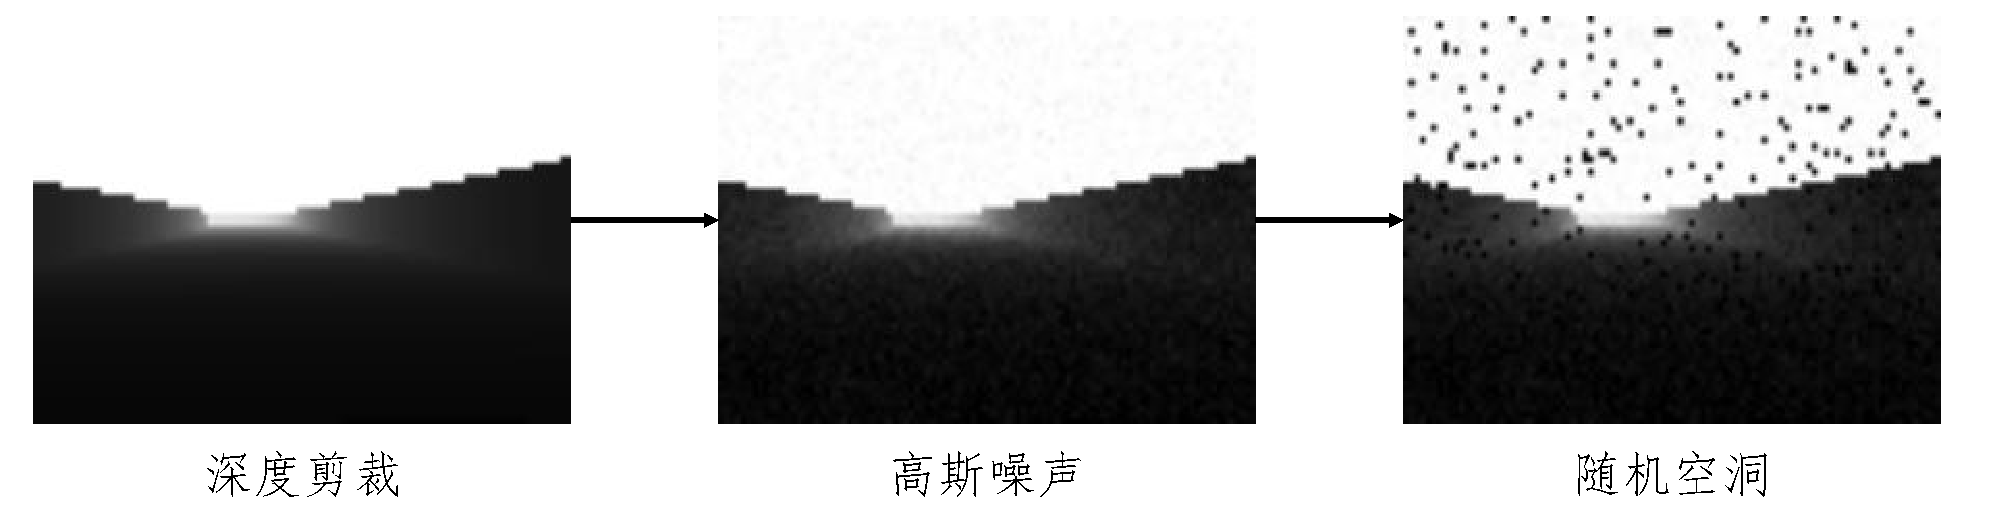
\includegraphics[width=0.8\linewidth]{figure/chapter3/add-noise.pdf}
    \caption{深度图像预处理}
    \label{fig:add-noise}
\end{figure}

\textbf{特权信息仿真：}二维激光雷达通过追踪车辆中心到不同方向的射线得到测量距离值。射线的数量为1080条，覆盖范围为$\theta_{fov}=270\degree$，最大测量值为$d_{max}=15m$。所有射线被分为$N_d=72$个区域，对应角度分辨率为$3.75\degree$，每个区域内的测量距离取该区域内所有射线的最小值。将所有测量距离合并后便得到了教师策略的观测中的二维激光雷达数据$\boldsymbol{d}_t$。$\boldsymbol{w}_t$包含$N_w=30$个赛道中心线采样点，每个采样点包含了相对于车辆坐标系的横向偏移量和纵向距离。相邻两个点之间的距离为$\Delta d=0.2m$。另外，我们对特权信息进行随机化，包括雷达扫描误差、线速度误差和角速度误差等，如表\ref{tab:domain-randomization}所示。

\textbf{深度图像仿真：}深度图像从Pybullet仿真器\cite{coumans2024python}中的车载摄像头获取，使用车辆的位置和姿态来计算摄像头的位姿，并通过赛道的URDF模型和仿真器的渲染功能生成深度图像。为了减小仿真和真实环境之间的视觉差距，我们在训练过程中对深度图像进行随机化处理，包括深度剪裁、高斯噪声、随机空洞等，如图\ref{fig:add-noise}所示。剪裁后的图像为$\tilde{\boldsymbol{I}}_t$，用于预训练VAE；原始图像为$\boldsymbol{I}_t$，用于训练学生策略。仿真和现实中的深度图像的分辨率均为$H\times W=64\times 96$，视场角为$58\degree\times87\degree$，深度剪裁范围为$0.28m-5m$，高斯噪声如表\ref{tab:domain-randomization}所示，随机空洞的概率为$0.2$。

\section{仿真与实车实验}
本章提出的方法在仿真和实车环境中进行了评估。首先，本方法在仿真中与其他竞速方法进行了对比实验，验证了其在不同赛道环境中的性能优势。然后，我们进行了消融实验，分析了方法中各个组件对整体性能的贡献。最后，我们将训练好的学生策略部署到实车系统中，验证了方法在仿真到实车迁移方面的有效性。

在仿真中，我们使用了不同赛道环境来评估方法的性能，如图\ref{fig:sim-track}所示。每个赛道环境都具有不同的布局和难度，以测试方法在不同环境中的泛化能力，赛道的参数如表\ref{tab:track-param}所示。另外，本章采用如下参数来评估竞速性能：（1）\textbf{完成时间}：完成一圈赛道所需的时间，单位为秒（s）。完成时间越短，表示竞速性能越好。（2）\textbf{成功率}：成功完成赛道的次数占总尝试次数的比例。成功率越高，表示避障性能越好。（3）\textbf{平均跃度}：平均跃度为竞速过程中车辆的平均跃度，跃度指加速度的导数，单位为$m/s^3$，表示轨迹的平滑度。
\begin{figure}[ht]
    \centering
    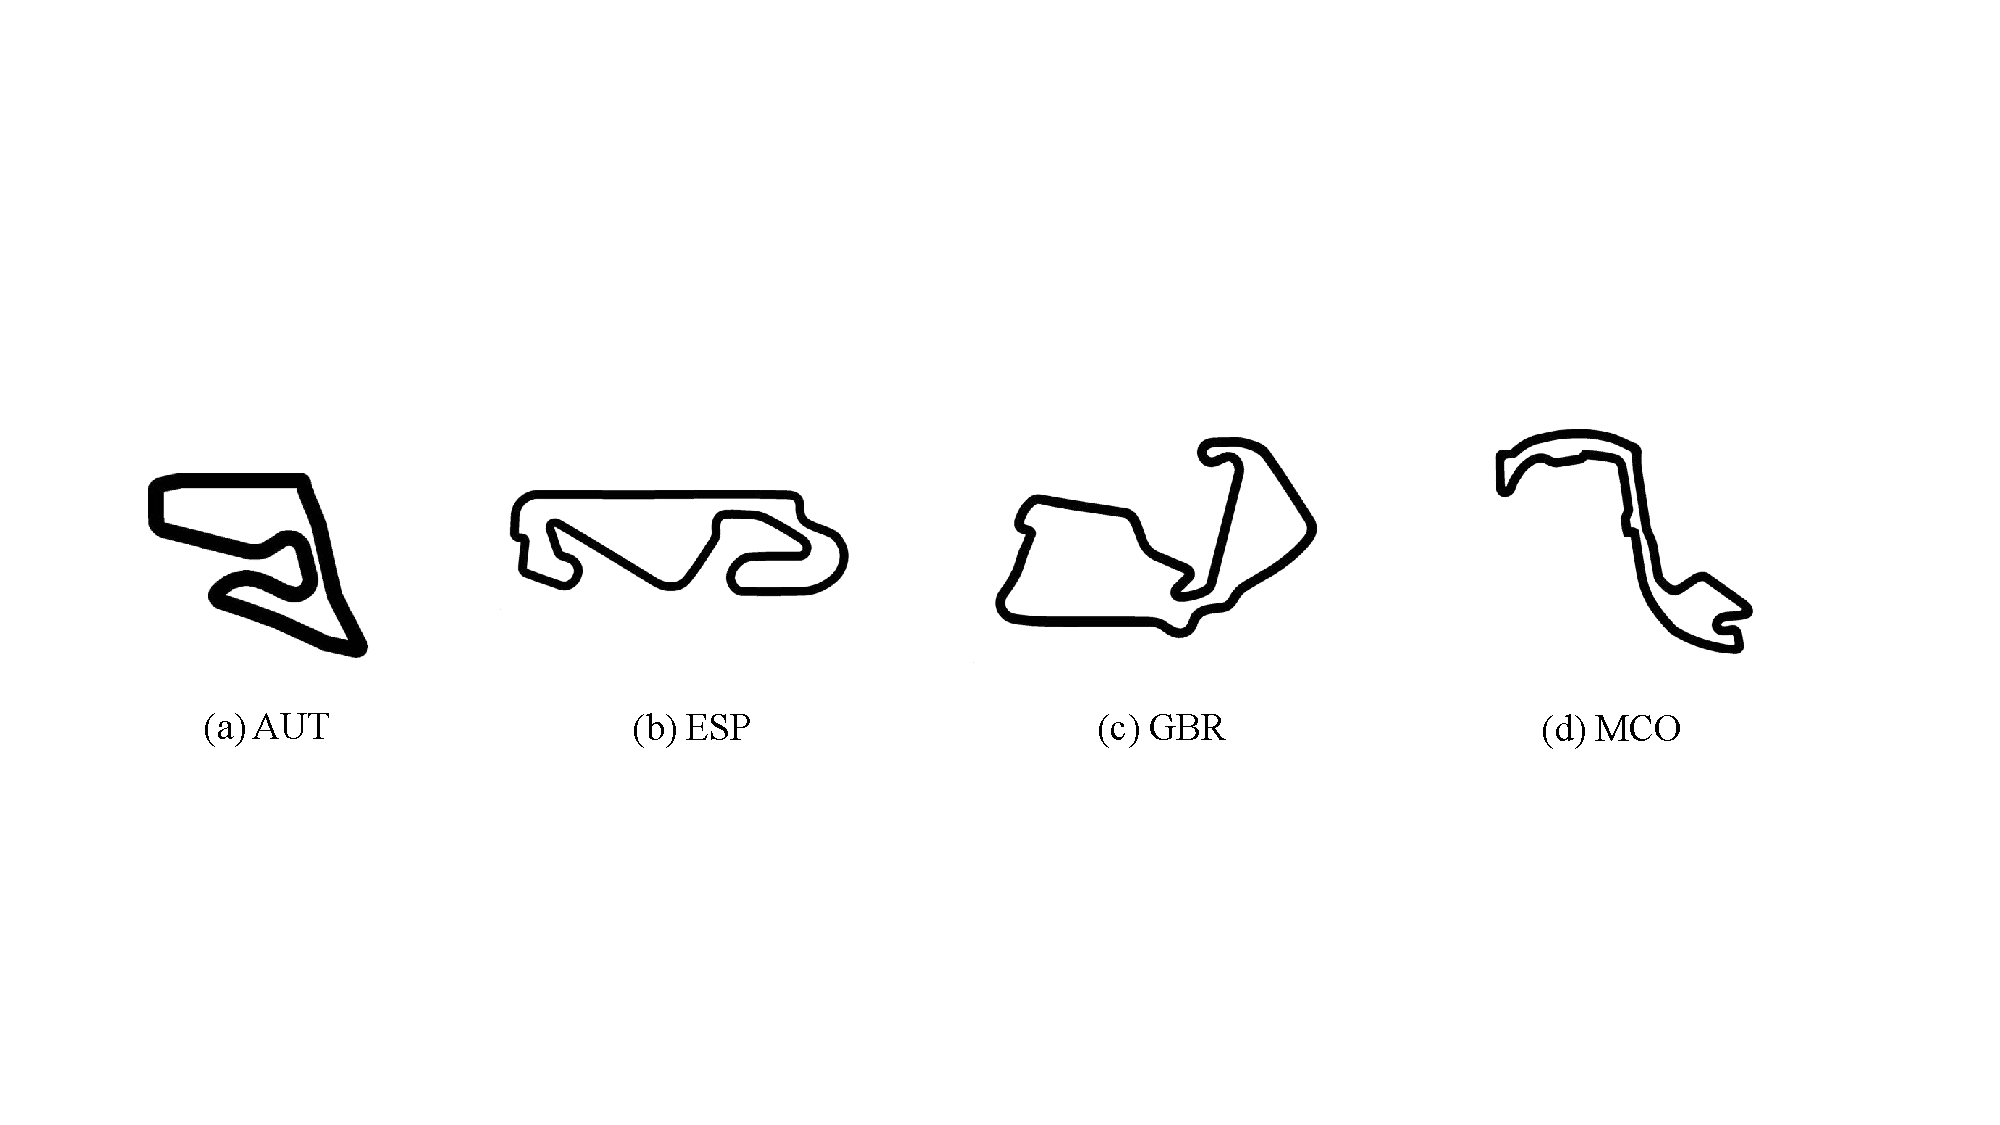
\includegraphics[width=1.0\linewidth]{figure/chapter3/newmap.pdf}
    \caption{不同赛道环境}
    \label{fig:sim-track}
\end{figure}
\begin{table}[ht]
    \caption{\label{tab:track-param}不同赛道环境的参数}
    \renewcommand{\arraystretch}{1.25}
    \begin{tabularx}{\linewidth}{X<{\centering} X<{\centering} X<{\centering} X<{\centering} X<{\centering}}
    \toprule[2pt]
        赛道名称 & AUT & ESP & GBR & MCO \\
    \midrule[1pt]
        赛道长度 [m] & 94.90 & 236.93 & 201.84 & 178.71 \\
        直道比例 [\%] & 64.92 & 58.98 & 59.45 & 60.60 \\
        弯道数量 [\mbox{-}] & 7 & 7 & 7 & 16 \\
    \bottomrule[2pt]
\end{tabularx}
\end{table}

本文的实验平台是一台$1:10$比例的遥控赛车，如图\ref{fig:visual-car-platform}所示。该赛车配有一个型号为Traxxas Velineon 3351R的无刷直流电机和一个型号为Traxxas 2075的舵机。赛车配备了一个Intel RealSense D435i深度摄像头，用于捕获前方环境的深度图像。赛车还配备了一个IMU传感器，用于测量车辆的加速度和角速度。所有传感器的数据通过ROS系统进行处理，并由一个机载计算平台（NVIDIA Jetson NX）运行学生策略来生成控制指令，最终发送给赛车的控制系统：VESC电子调速器，实现实时的运动控制。
\begin{figure}[ht]
    \centering
    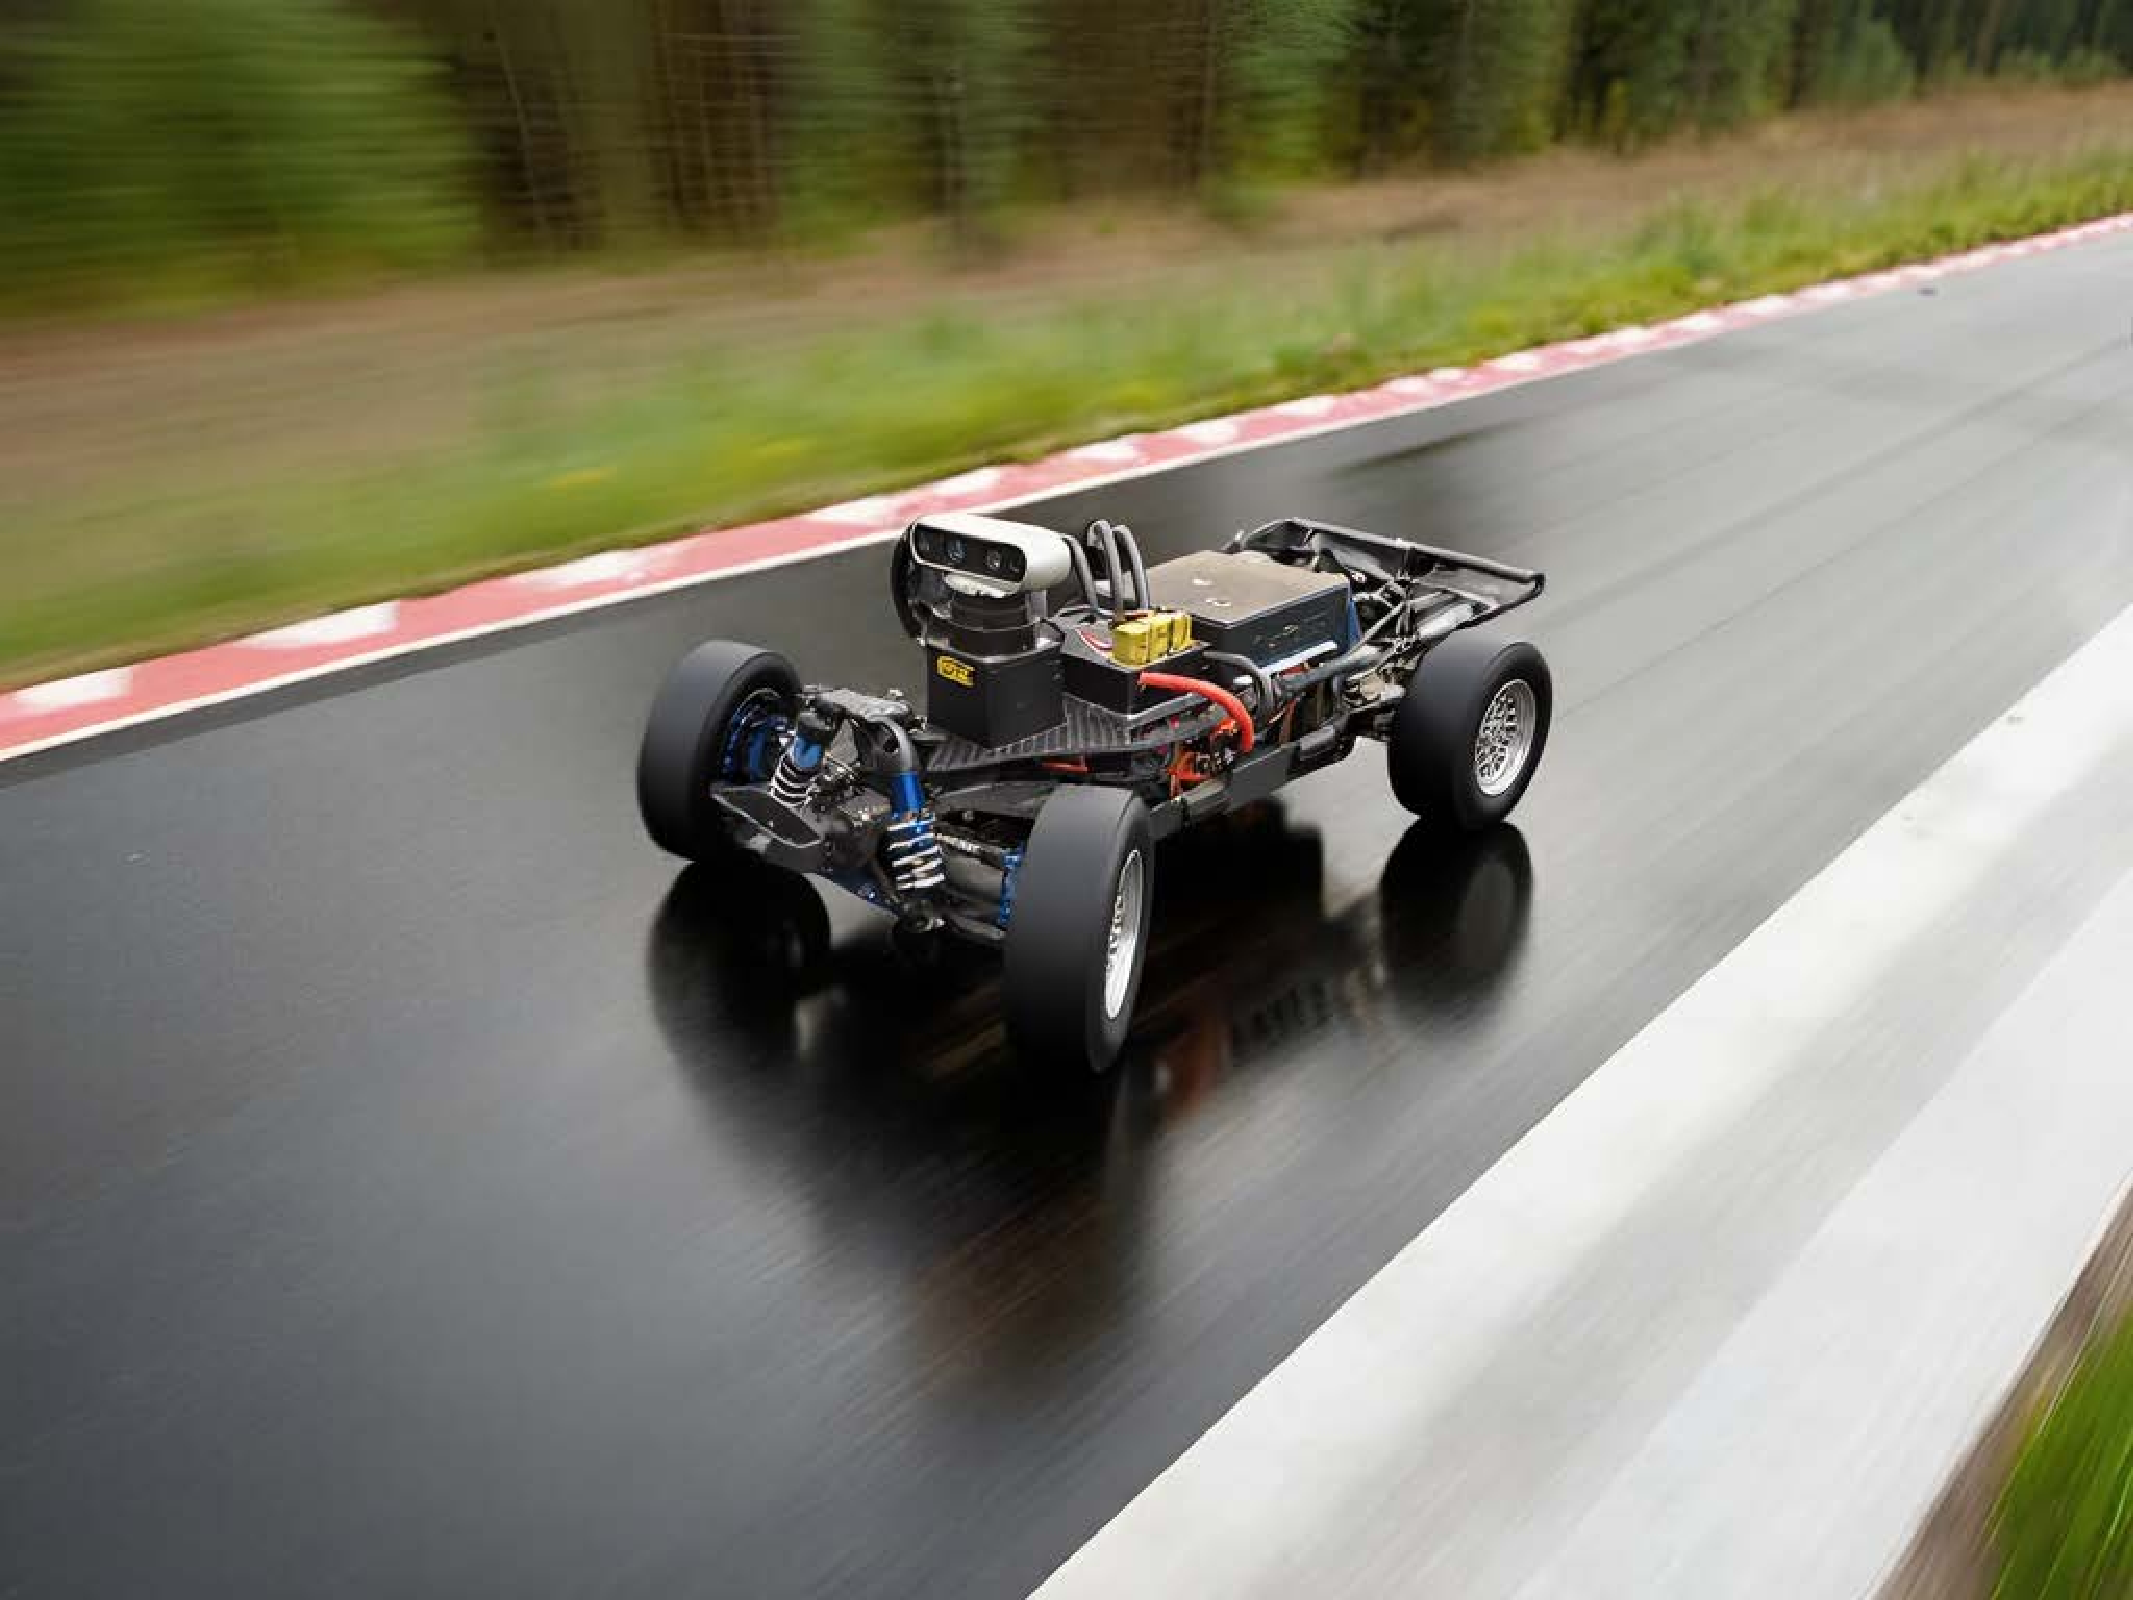
\includegraphics[width=0.5\linewidth]{figure/chapter3/car.pdf}
    \caption{基于视觉的赛车实验平台}
    \label{fig:visual-car-platform}
\end{figure}

\subsection{竞速效果对比实验}
本节展示了基于视觉的竞速方法和其他方法的对比试验结果。本文的方法在不同赛道环境下的竞速轨迹如图\ref{fig:student_traj}所示。可以看出，本文的方法能够在不同赛道环境中生成平滑且高效的竞速轨迹，并且在弯道处能够保持较高的速度，从而实现了较短的完成时间和较高的成功率。对比实验的基线方法选择如下\footnote{MPCC和TAL方法的复现是基于以下仓库源码: {\tt\small https://github.com/BDEvan5/f1tenth\_benchmarks.}}：（1）基于优化的方法：模型预测轮廓控制（Model Predictive Contour Control，简称MPCC）\cite{liniger2015optimization}，该方法已知全局状态以及赛道中线、边界等信息，使用非线性优化方法在线求解最优控制问题；（2）数据驱动的方法：轨迹辅助学习（Trajectory-Aided Learning，简称TAL）\cite{evans2023high}，该方法利用预先生成的轨迹数据来辅助强化学习算法的训练，通过激光雷达数据和车辆状态信息来学习竞速策略；（3）本文提出的教师策略方法（Teacher），该方法使用预先提取的特权信息作为输入，采用强化学习的方法训练控制策略；（4）本文提出的学生策略方法（Student），该方法使用车载摄像头获取的视觉信息作为输入，通过知识蒸馏的方法从教师策略中学习控制策略。四个赛道用于评估基线方法的竞速效果，每个方法在每个赛道上进行了40次独立的试验，统计了完成时间、成功率和平均跃度等指标。
\begin{figure}[t]
\centering
\subfloat[AUT]{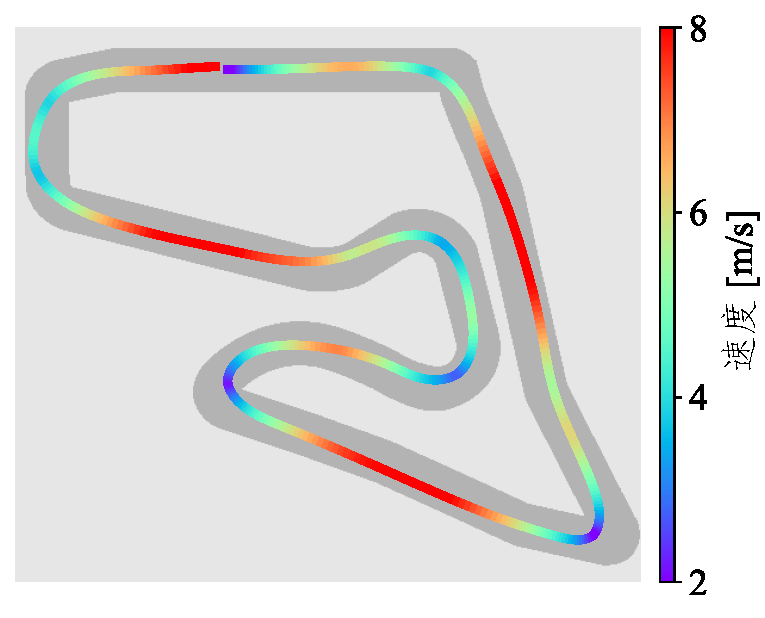
\includegraphics[width=0.4\linewidth]{figure/chapter3/student_aut.pdf}}
\subfloat[ESP]{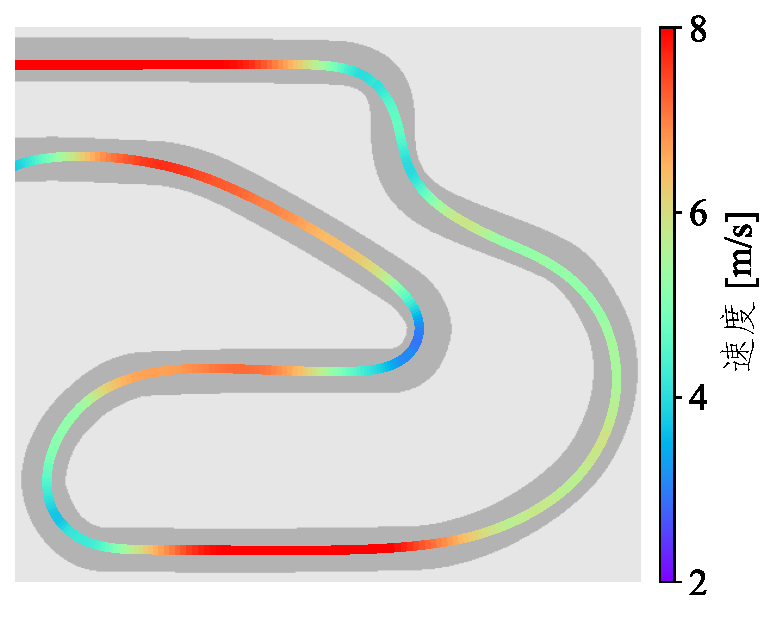
\includegraphics[width=0.4\linewidth]{figure/chapter3/student_esp.pdf}}

\subfloat[GBR]{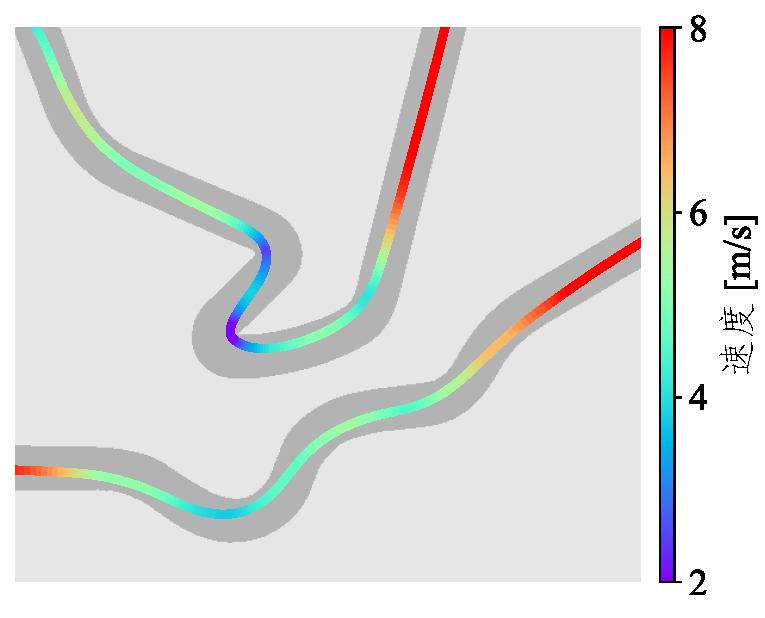
\includegraphics[width=0.4\linewidth]{figure/chapter3/student_gbr.pdf}}
\subfloat[MCO]{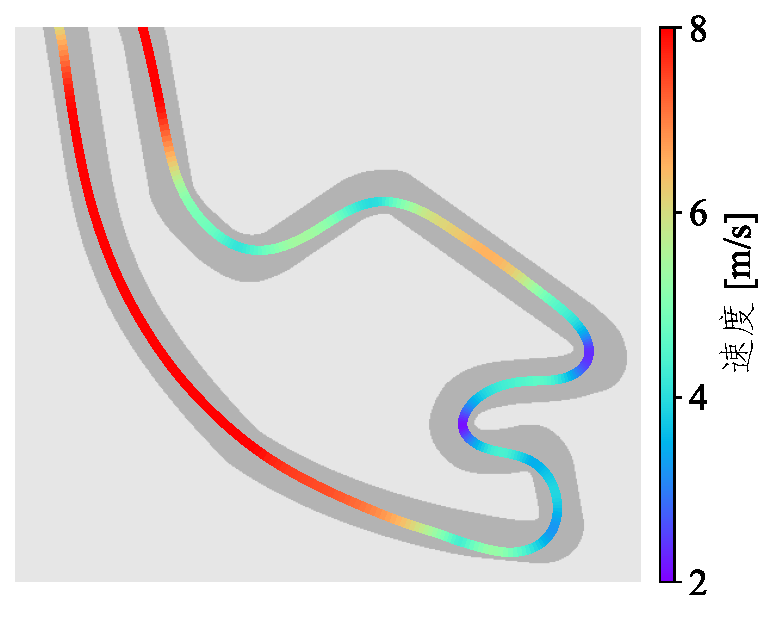
\includegraphics[width=0.4\linewidth]{figure/chapter3/student_mco.pdf}}
\caption{基于视觉的竞速方法在不同赛道环境下的轨迹}
\label{fig:student_traj}
\end{figure}

\begin{table}[t]
    \caption{\label{tab:lap-time}不同方法在不同赛道环境下的完成时间}
    \renewcommand{\arraystretch}{1.25}
    \setlength{\tabcolsep}{18pt}{
    \begin{tabular}{c|cccc}
    \toprule[2pt]
        \multirow{2}{*}{\textbf{基线方法}} & \multicolumn{4}{c}{\textbf{不同赛道下的完成时间[s]}}\\
        & AUT & ESP & GBR & MCO \\
    \midrule
        MPCC & 16.93$\pm$0.42 & 39.57$\pm$0.36 & 35.42$\pm$0.57 & 32.07$\pm$0.49 \\
        TAL & 19.67$\pm$0.54 & 45.84$\pm$0.49 & 39.67$\pm$0.78 & 35.04$\pm$0.89 \\
        Teacher & \textbf{16.19}$\pm$\textbf{0.46} & 37.84$\pm$0.38 & \textbf{32.57}$\pm$\textbf{0.47} & \textbf{29.72}$\pm$\textbf{0.41} \\
        Student & 16.27$\pm$0.47 & \textbf{37.74}$\pm$\textbf{0.41} & 32.84$\pm$0.44 & 30.07$\pm$0.43 \\
    \bottomrule[2pt]
    \end{tabular}}
\end{table}
\begin{figure}[ht]
    \centering
    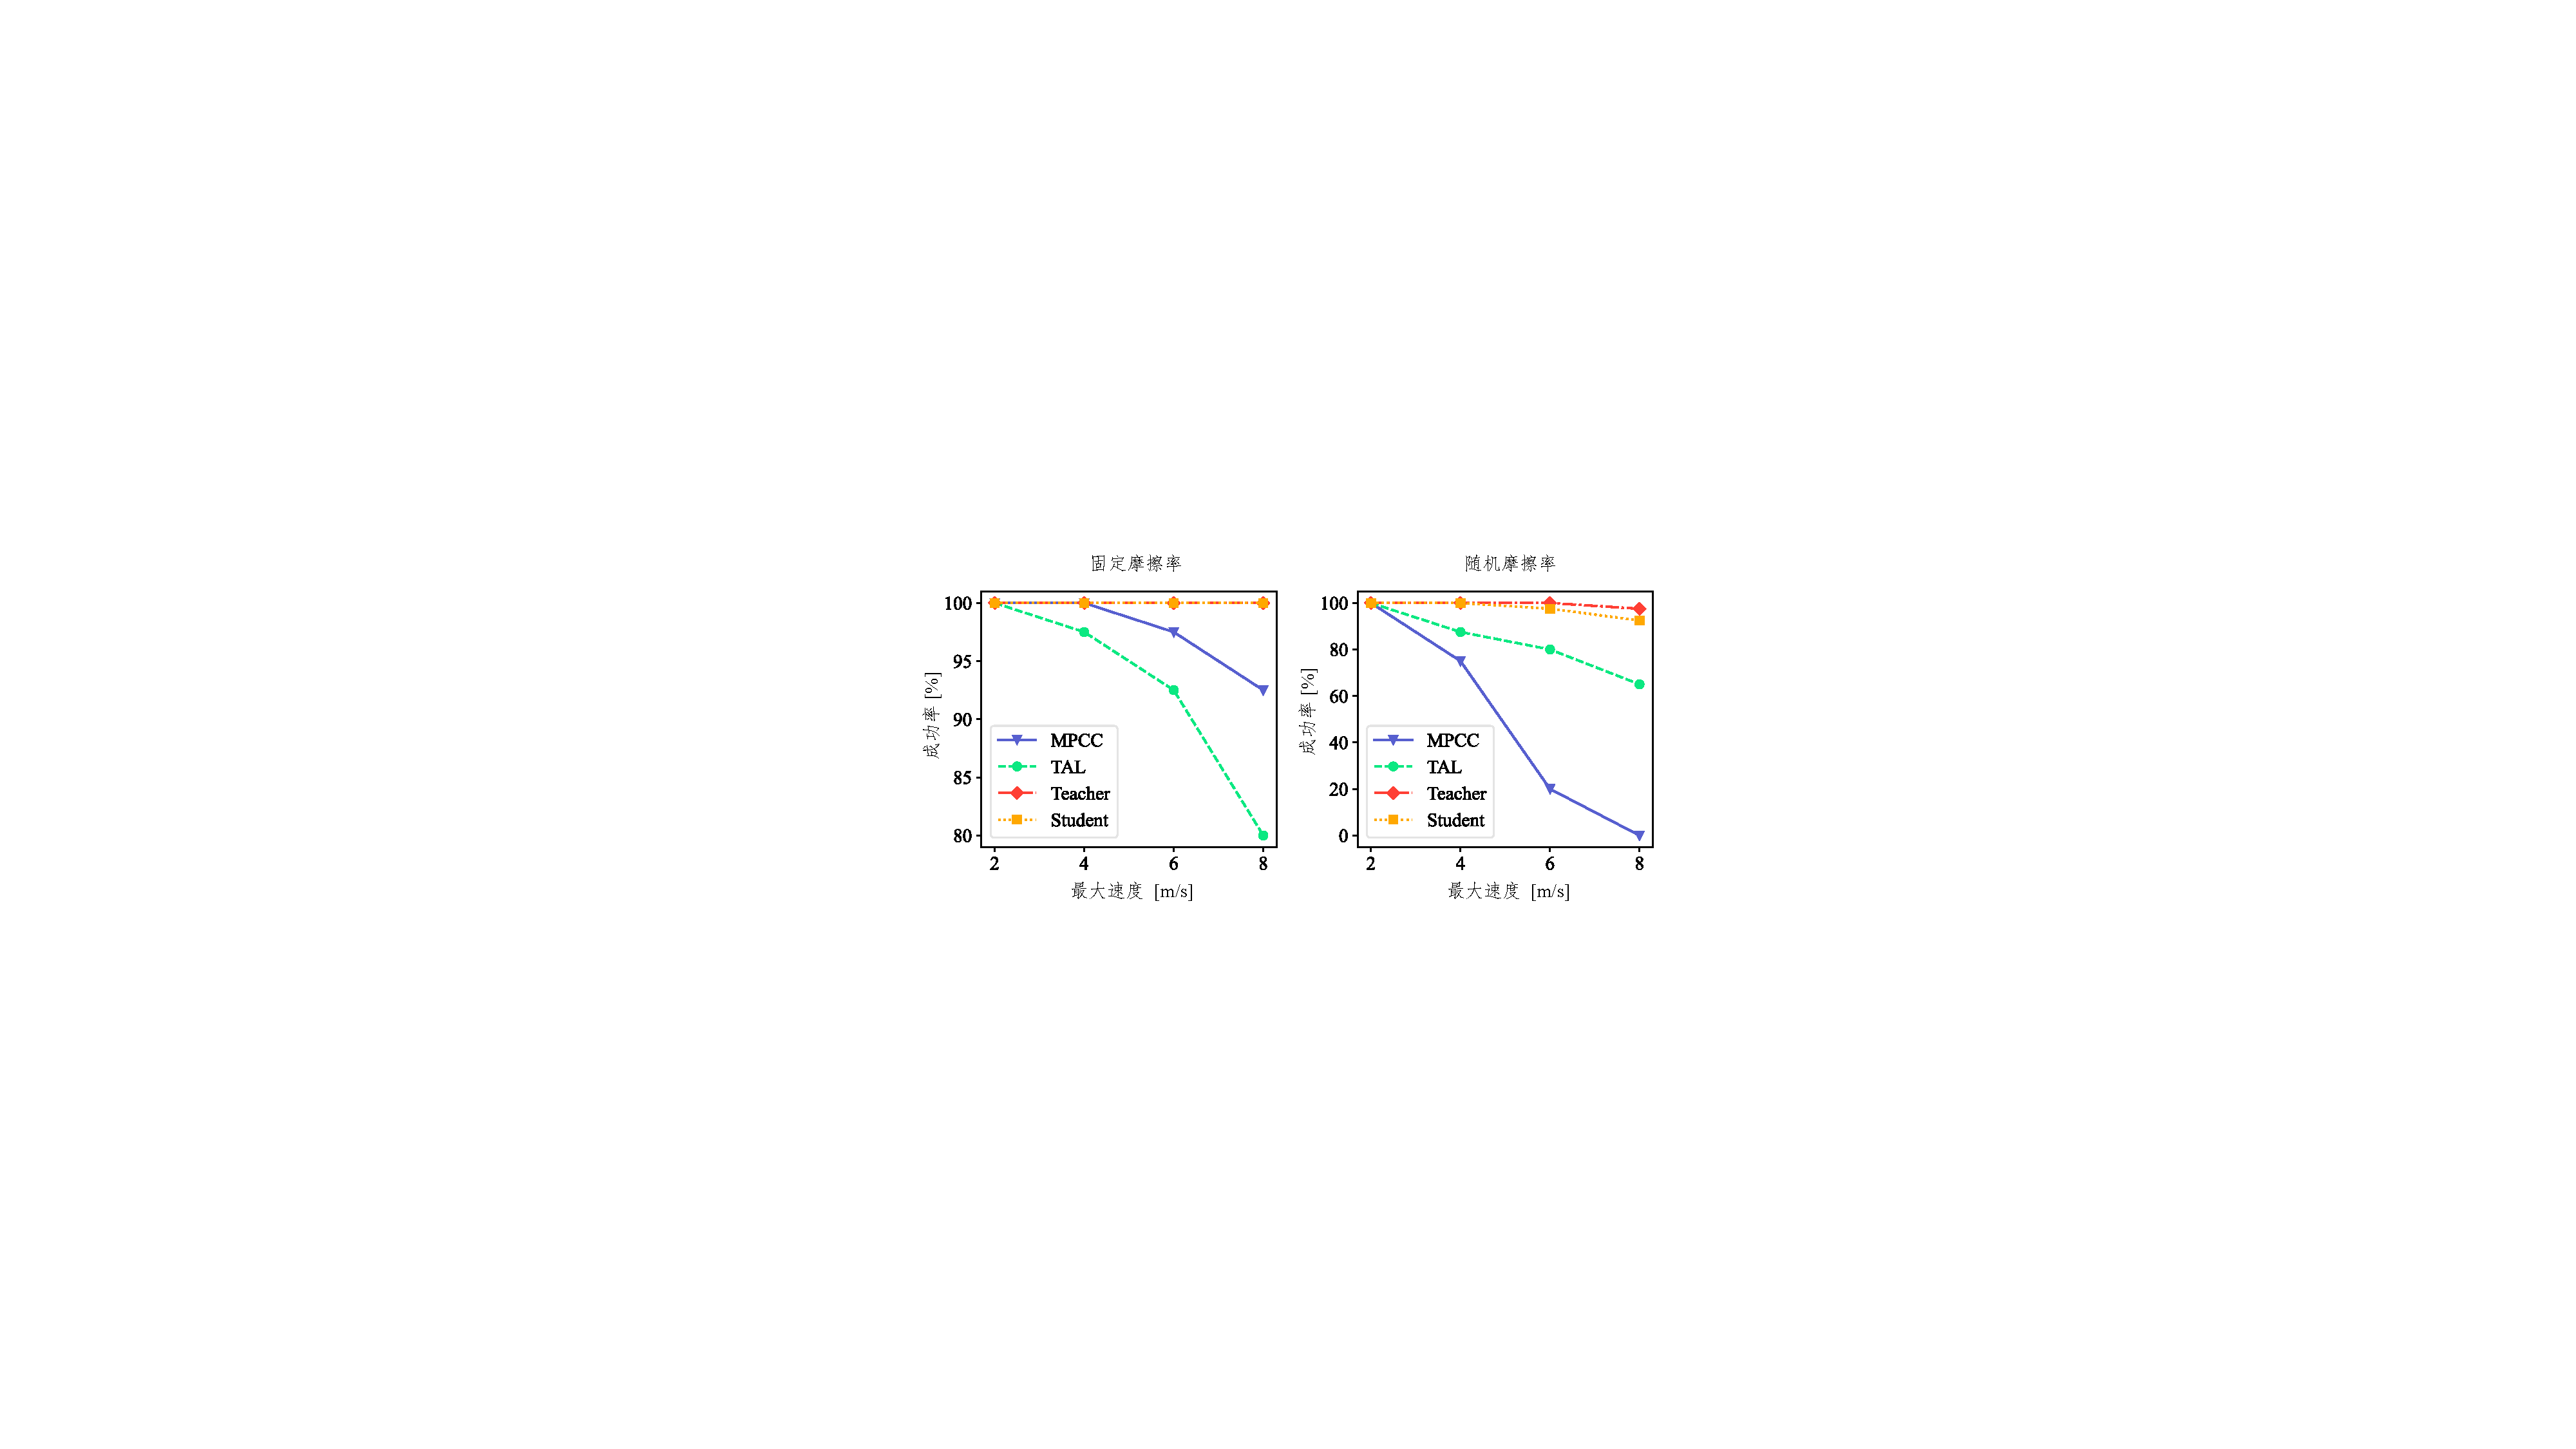
\includegraphics[width=0.85\linewidth]{figure/chapter3/success.pdf}
    \caption{不同方法在不同最大速度下在MCO赛道上的成功率}
    \label{fig:success}
\end{figure}
\begin{figure}[ht]
    \centering
    \subfloat[轨迹可视化]{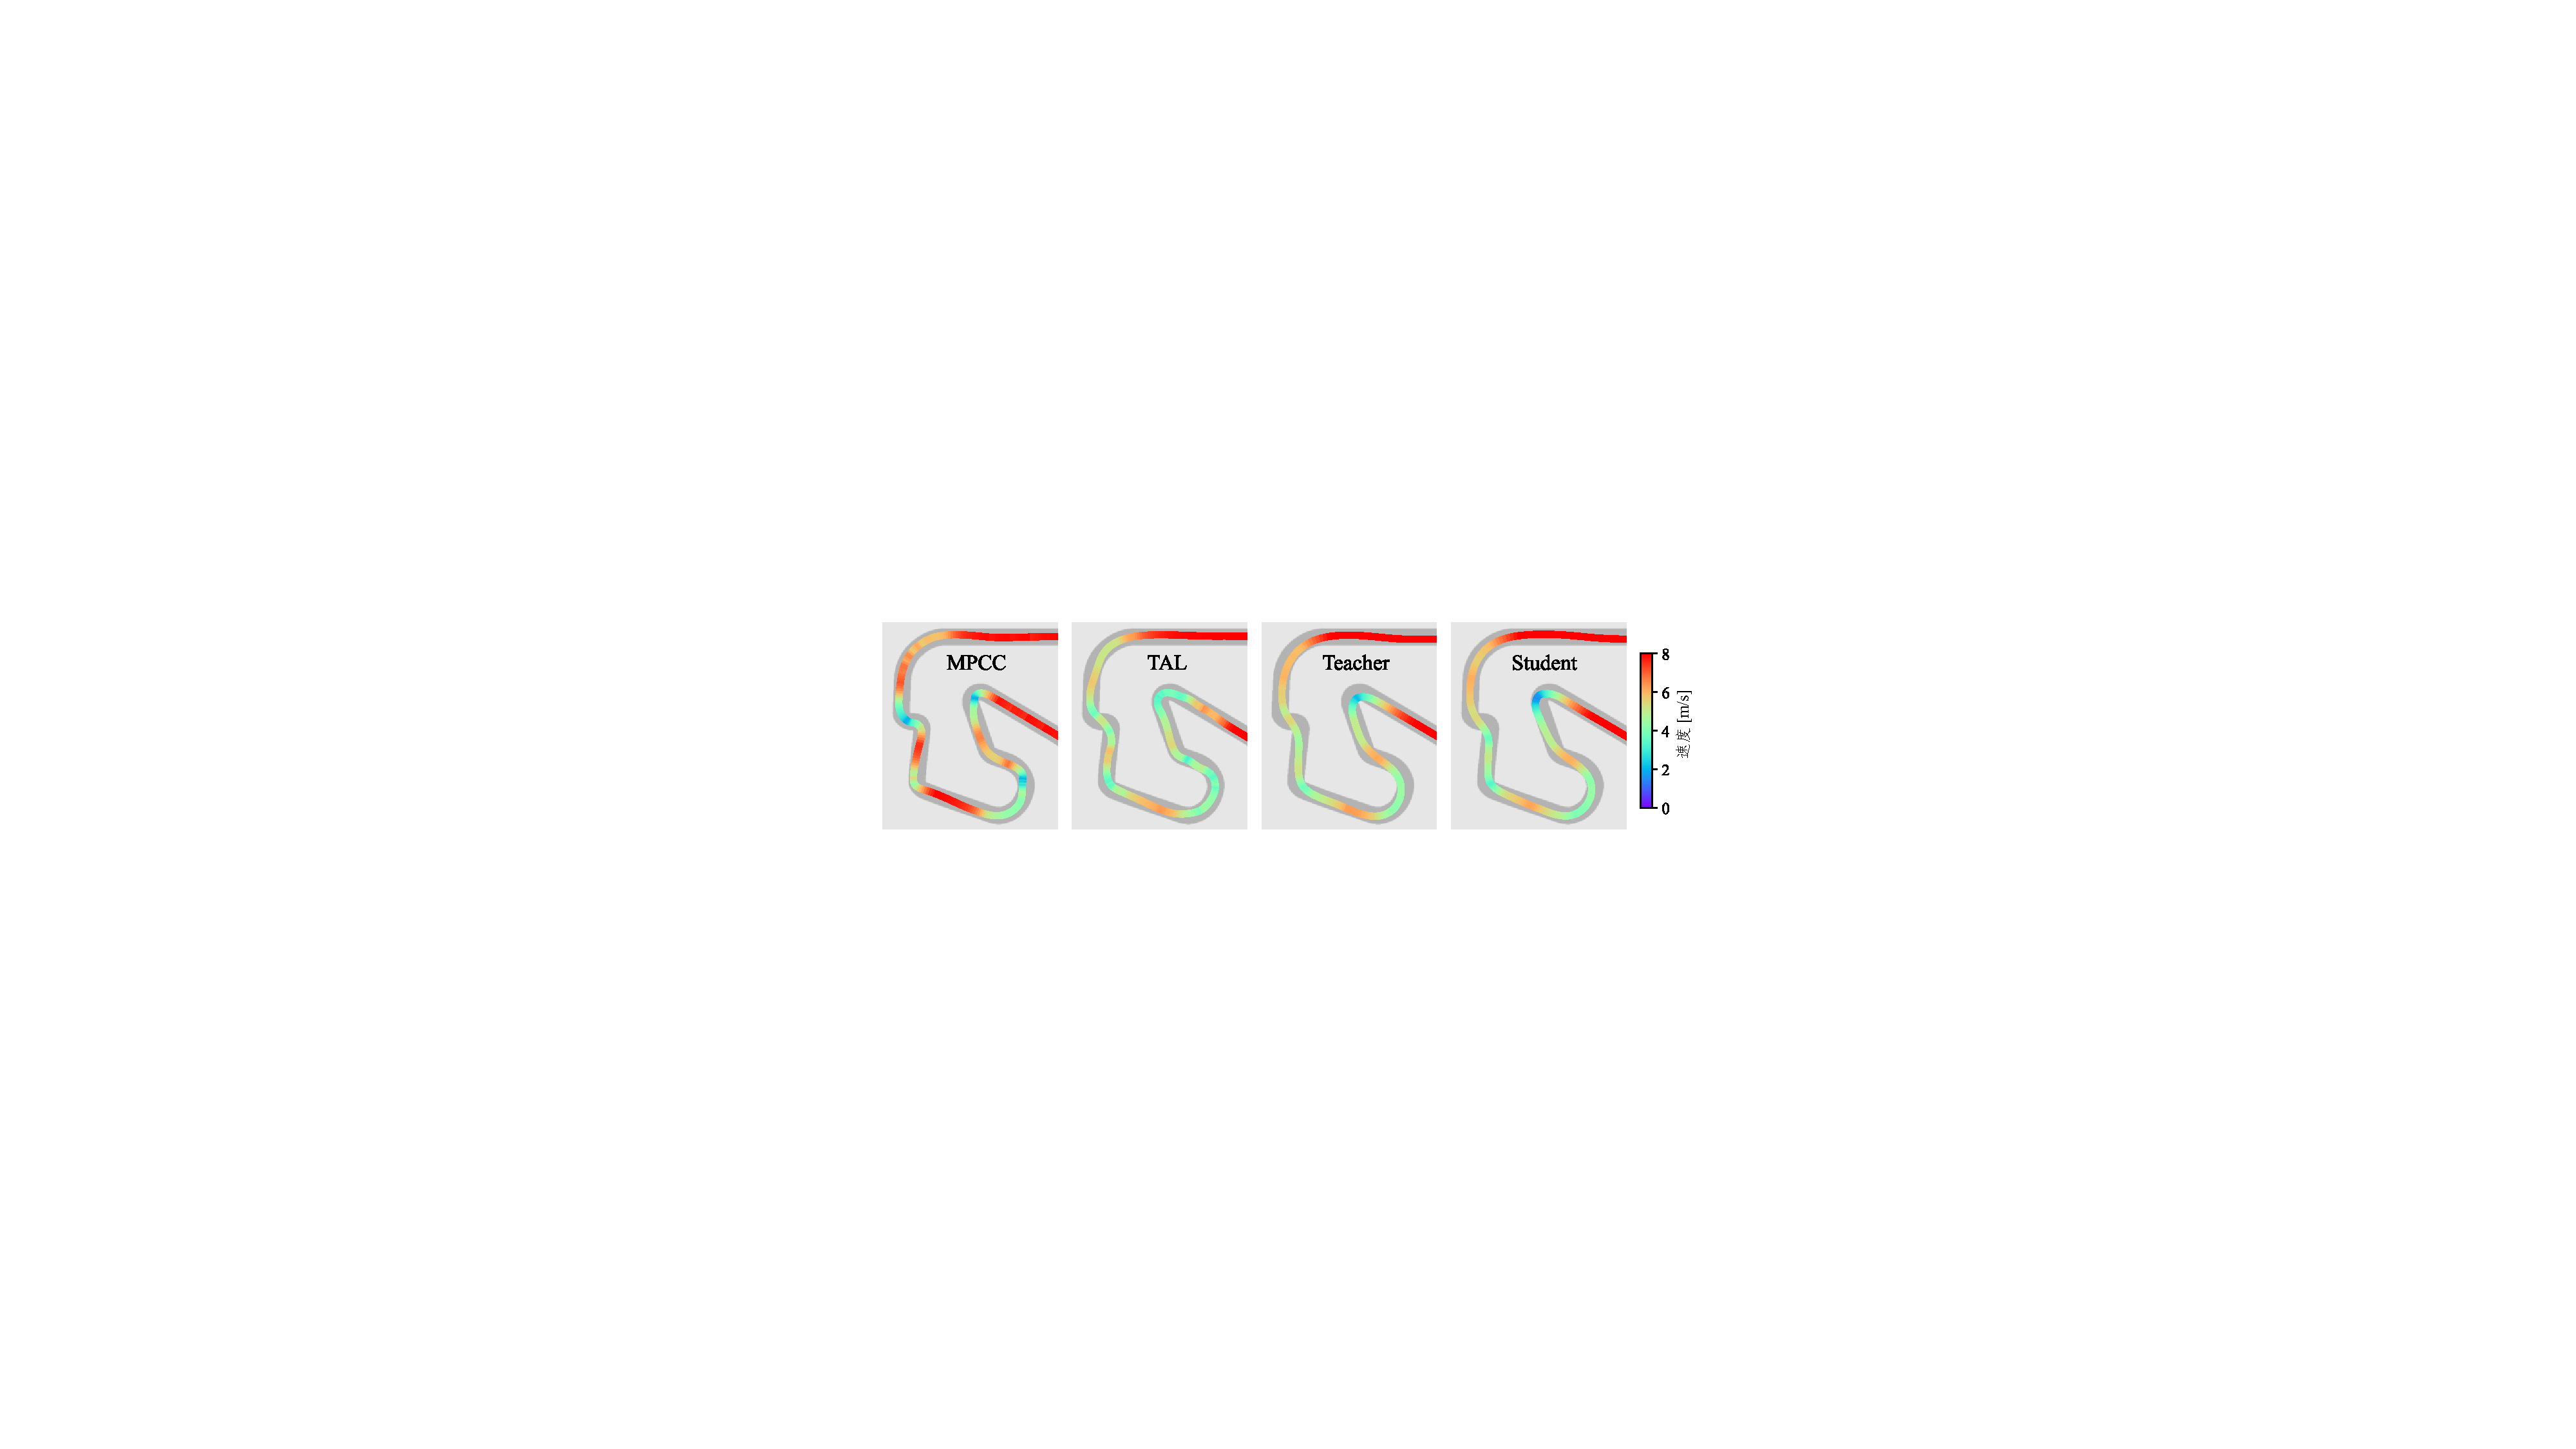
\includegraphics[width=0.9\linewidth]{figure/chapter3/compare.pdf}}

    \subfloat[平均跃度]{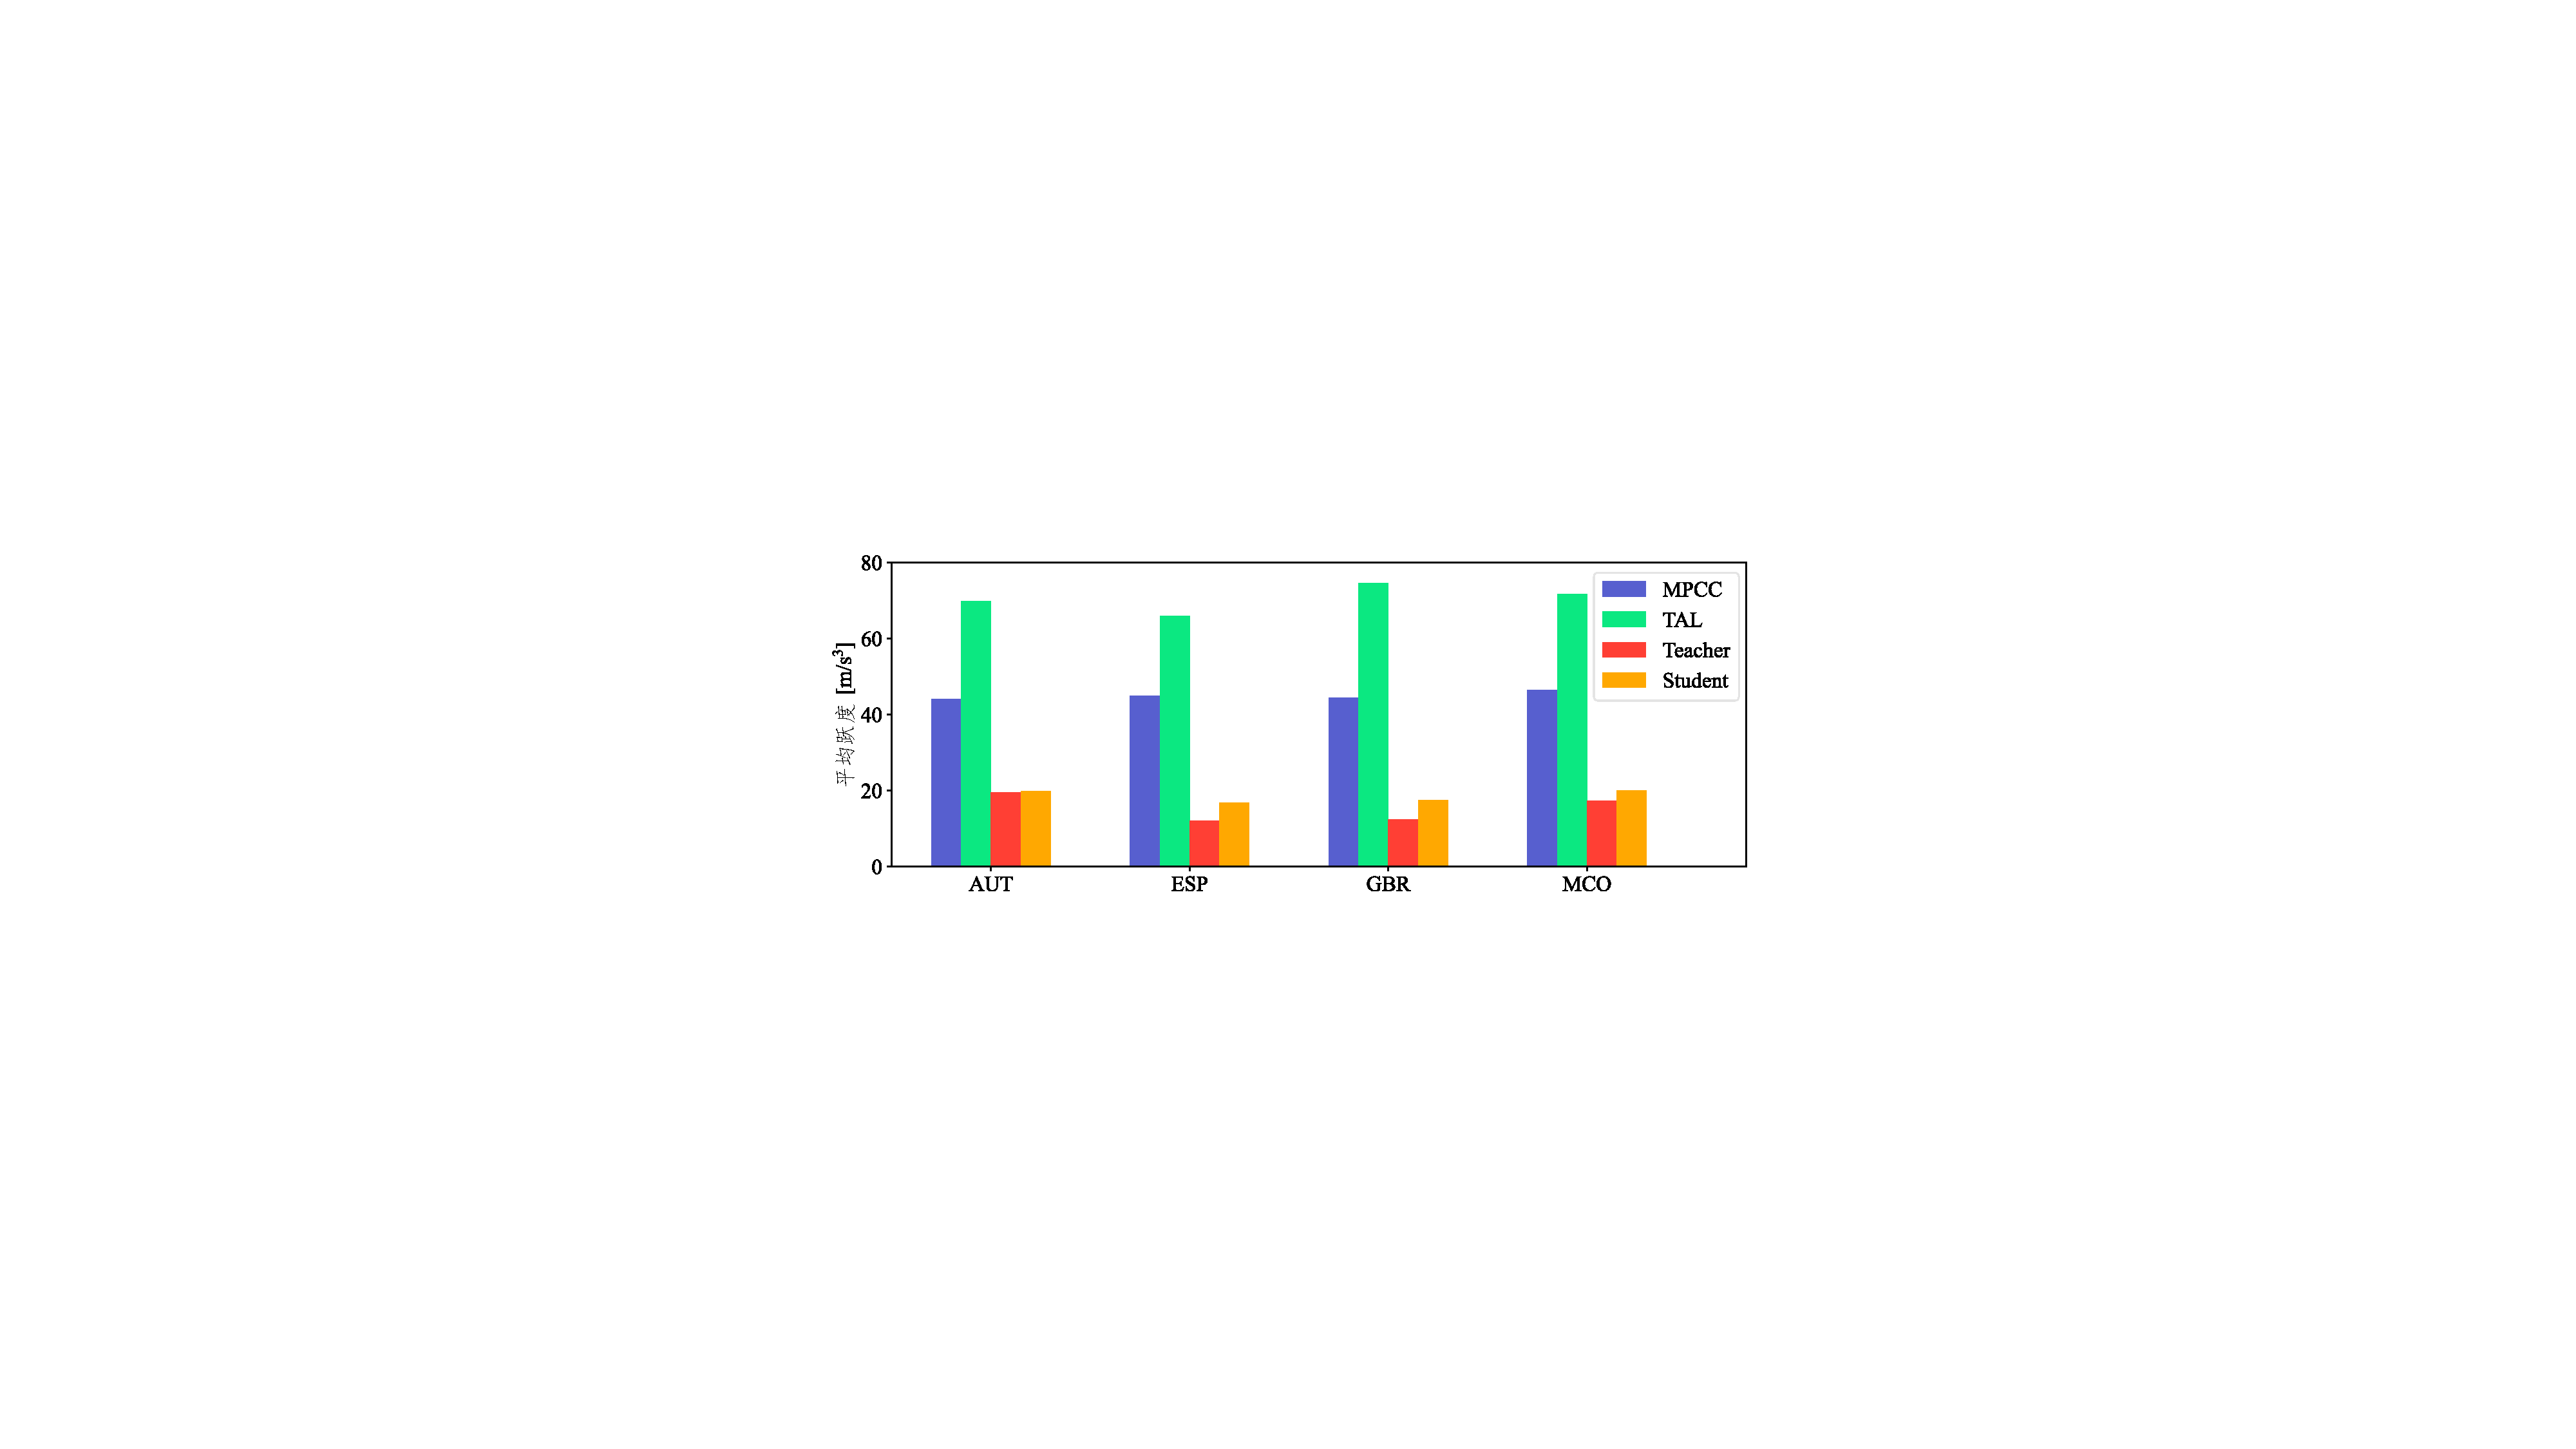
\includegraphics[width=0.8\linewidth]{figure/chapter3/jerk.pdf}}
    \caption{不同方法在ESP赛道上的轨迹比较}
    \label{fig:esp-traj}
\end{figure}

\textbf{完成时间：}表\ref{tab:lap-time}展示了不同方法在不同赛道环境下的完成时间。可以看出，本文提出的教师策略方法在所有赛道环境中大都取得了最短的完成时间，表明其在竞速性能方面具有明显的优势。学生策略方法的完成时间与教师策略方法非常接近，说明通过知识蒸馏训练的学生策略能够有效地学习教师策略的控制行为，从而实现高效的竞速。基线方法中，TAL方法的完成时间最长，盲目地模仿基于模型的方法使其缺乏赛道进度的奖励；MPCC方法已知全局信息，完成时间相对较短，但仍然不如本文提出的方法，可能是因为MPCC方法过于强调最小化轮廓误差，导致了保守的竞速轨迹。

\textbf{成功率：}为了评估不同方法的避障性能，我们在MCO赛道上测试了不同方法在不同最大速度下的成功率，如图\ref{fig:success}所示。实验分为两组，第一组在固定摩擦率$\mu=0.8$的路面上进行测试，第二组在随机化摩擦率$\mu\sim\mathcal{N}(0.8, 0.1^2)$的路面上进行测试。可以看出，在固定摩擦率的路面上，所有方法的成功率都在$80\%$以上，本文提出的方法表现最好。但在随机摩擦率的路面上，基线方法的成功率显著下降。MPCC方法由于对准确模型的强依赖性，在不确定环境中的表现较差；TAL方法虽然在某些情况下表现尚可，但整体性能不如本文提出的方法。本文提出的方法仍然保持较高的成功率，表明其在不确定环境中的鲁棒性更强。这可能是因为本文的方法在训练过程中引入了域随机化技术，使得模型能够适应不同的环境变化，从而提高了其泛化能力。

\textbf{平均跃度：}图\ref{fig:esp-traj}展示了不同方法在ESP赛道上的轨迹比较以及平均跃度。可以看出，本文提出的方法生成的竞速轨迹更加平滑，平均跃度较低，表明其在控制策略的平滑性方面具有优势。教师策略方法的平均跃度略低于学生策略方法，这可能是因为教师策略直接使用特权信息进行决策，而学生策略需要通过视觉输入来推断环境状态，可能会引入一些不确定性，从而导致略高的跃度。基线方法中，MPCC方法的平均跃度较高，可能是因为其过于强调最小化轮廓误差，导致了较为激烈的控制输入变化；TAL方法的平均跃度也较高，可能是因为其依赖于预先生成的轨迹数据，在某些情况下可能无法很好地适应环境变化，从而导致较为激烈的控制输入变化。

\textbf{数据效率：}为了展现本文方法在视觉控制任务中的数据效率，我们还比较了不同方法在训练过程中的累积奖励变化。两种基于视觉的强化学习算法在同样的环境中进行训练：（1）使用PPO2算法训练一个基于CNN的策略网络，并且使用RNN神经网络来处理部分可观性（CNN-PPO-RNN）；（2）使用PPO2算法训练一个基于预训练VAE的策略网络，并且使用RNN神经网络来处理部分可观性（VAE-PPO-RNN）。两种强化学习算法使用与本文方法相同的奖励函数，累积奖励随训练步数的变化如图\ref{fig:training-reward}所示。一条运动轨迹最长为600步，训练过程中的累积奖励是每条轨迹的奖励总和。可以看出，本文方法在训练过程中能够更快地收敛到较高的累积奖励，这表明其在视觉控制任务中的数据效率更高。教师策略由于使用了特权信息，能够更快地学习到有效的控制策略，且观测为低维的向量，只需要少量的训练数据就能学到较好的策略；学生策略由于使用视觉预训练和知识蒸馏技术，数据效率甚至更高，且累积奖励和教师策略相当。相比之下，CNN-PPO-RNN在训练过程中累积奖励的增长较慢，难以收敛，这可能是因为该方法需要从高维的视觉输入中学习有效的特征表示，训练复杂且不稳定；VAE-PPO-RNN累积奖励的增长相对较快，但最终的累积奖励仍然不如本文方法，这可能是因为该方法虽然使用了预训练VAE来提取视觉特征，但仍然缺乏教师策略提供的监督信号。
\begin{figure}[ht]
    \centering
    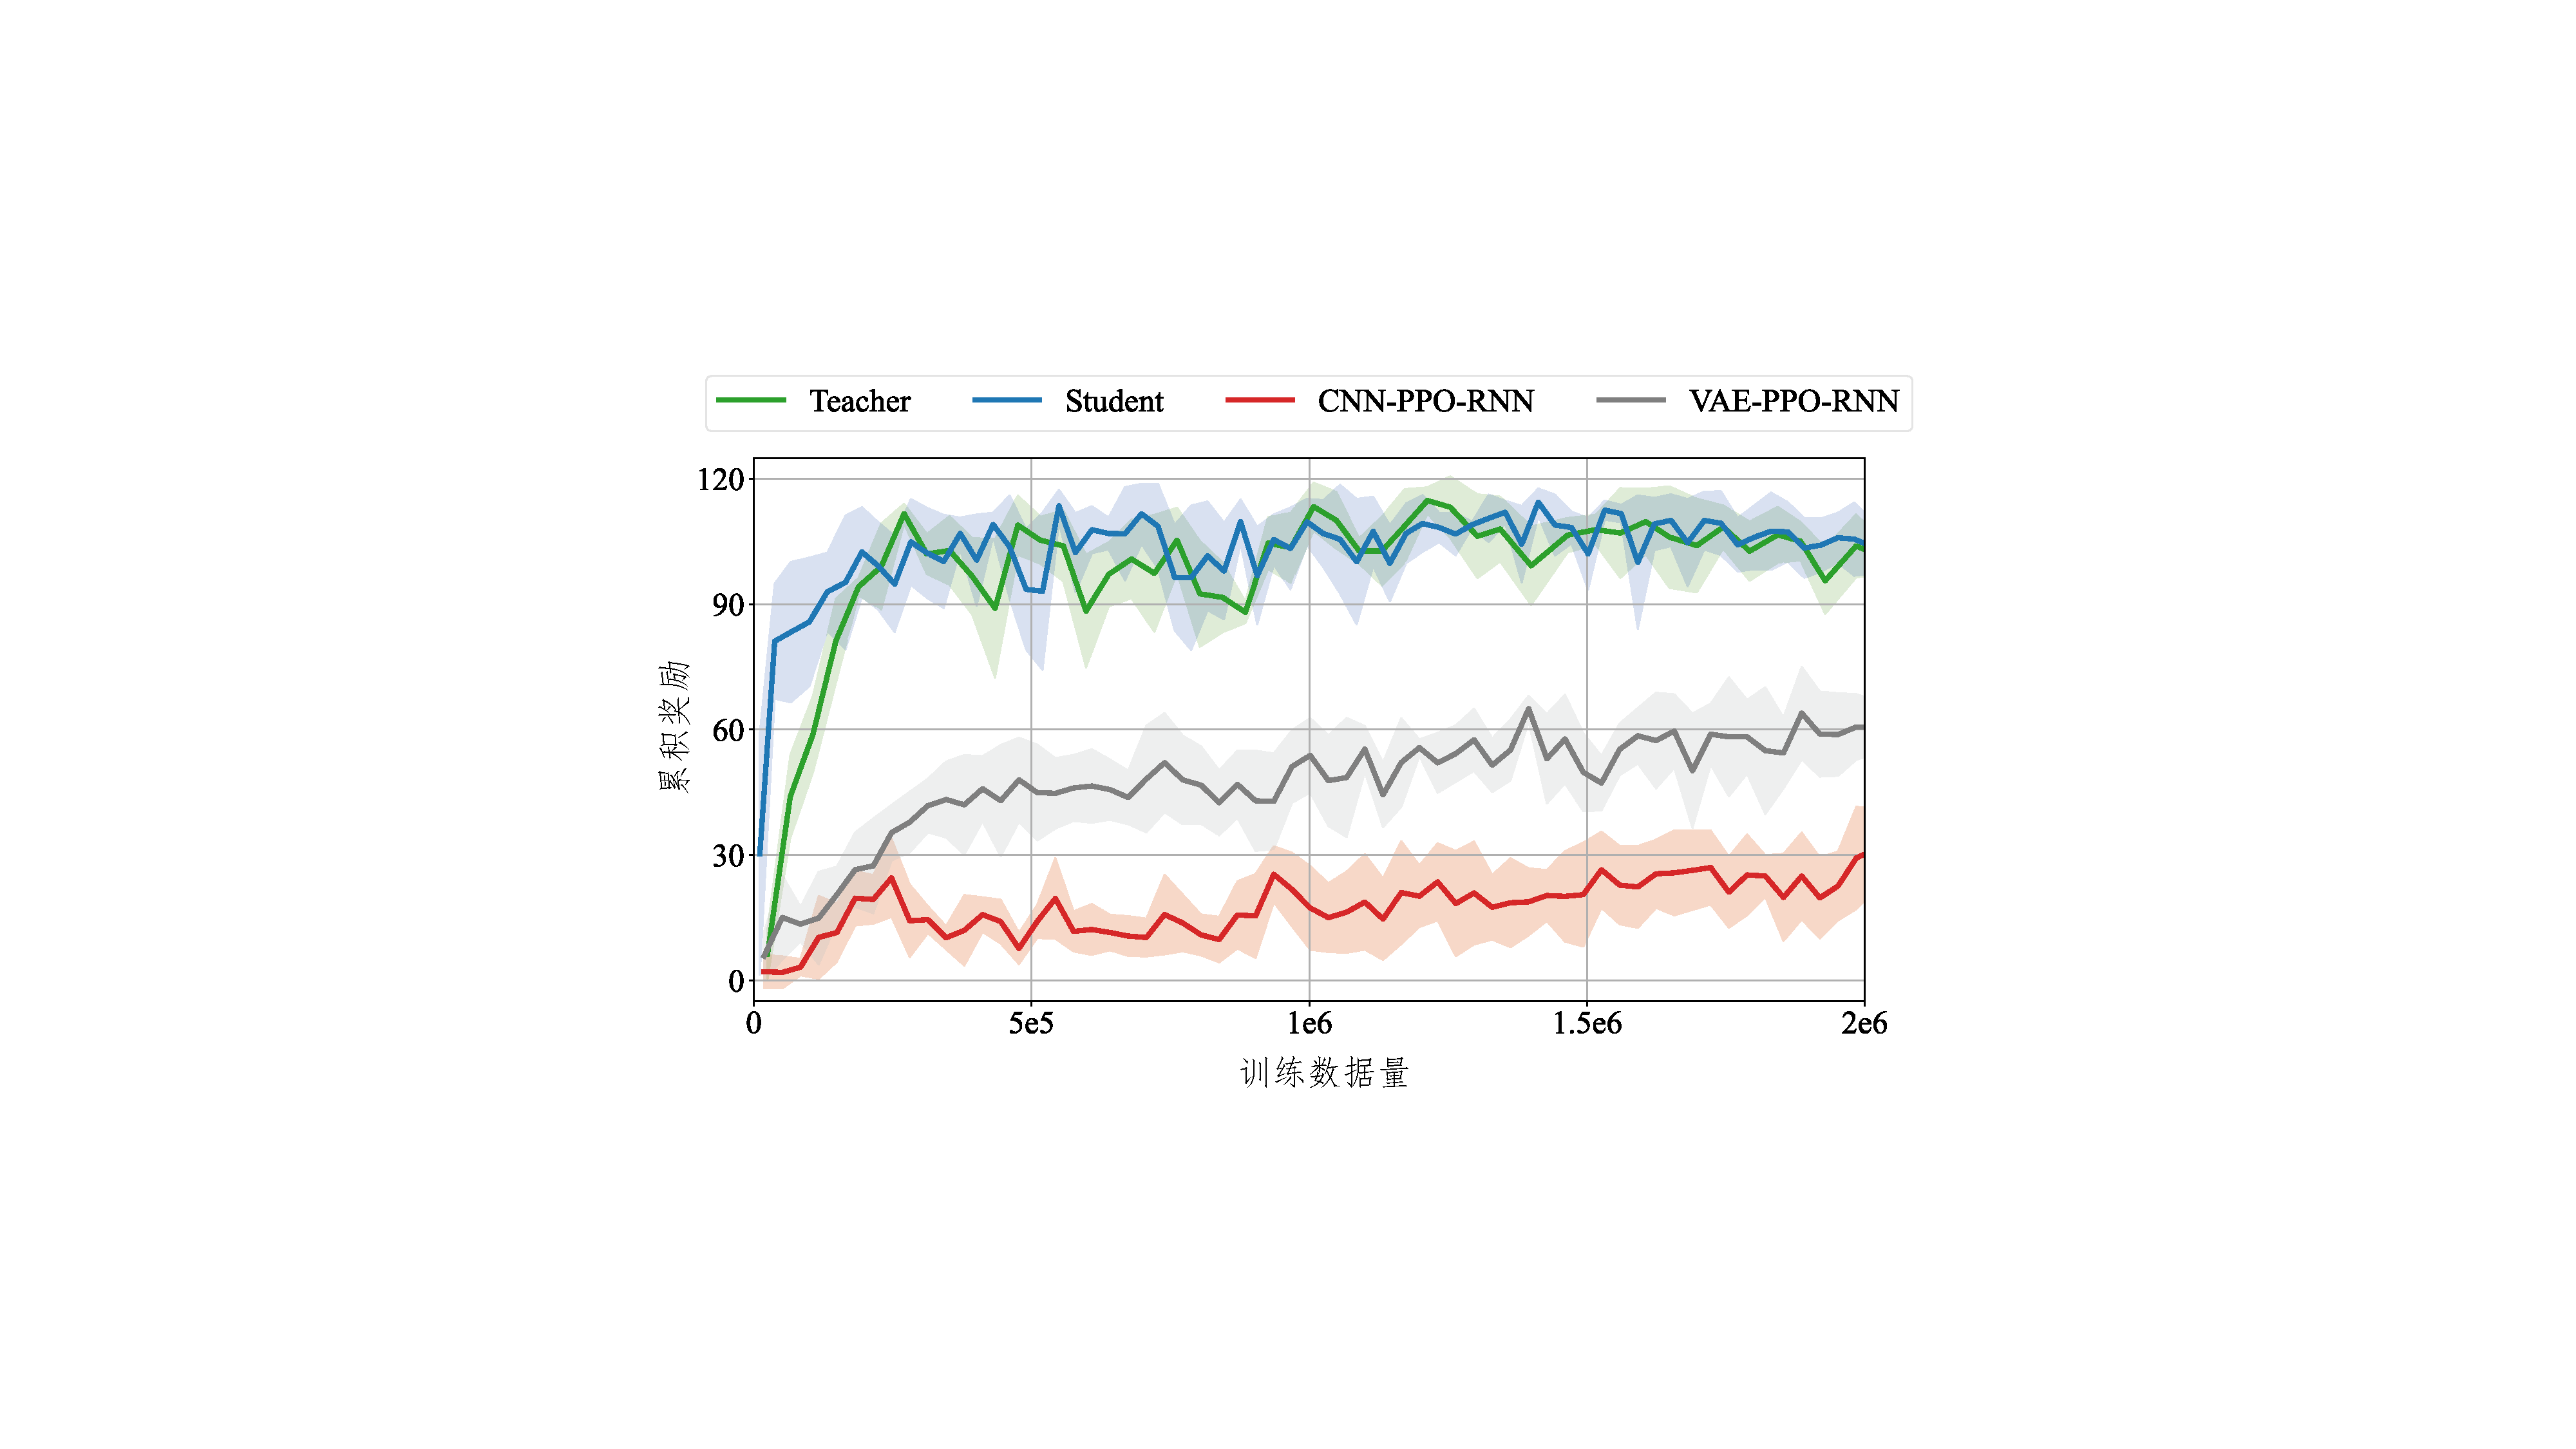
\includegraphics[width=0.73\linewidth]{figure/chapter3/reward.pdf}
    \caption{不同方法在训练过程中的累积奖励曲线}
    \label{fig:training-reward}
\end{figure}

\subsection{消融实验}
\begin{table}[ht]
\renewcommand{\arraystretch}{1.25}
\caption{不同策略在MCO赛道下的消融实验}
\centering
\setlength{\tabcolsep}{12pt}{
    \begin{tabular}{cc|ccc}
    \toprule
        & & 成功率[\%] & 完成时间[s] & 平均跃度[$m/s^3$]\\
    \midrule
        \multirow{2}{*}{\textbf{本文方法}} & Teacher & 100 & 29.72 & 20.07\\
        ~ & Student & 100 & 30.07 & 20.43\\
    \midrule
        \multirow{1}{*}{\textbf{无GRU}} & Student & 67.5 & 32.03 & 28.28\\
    \midrule
        \multirow{2}{*}{\textbf{无先验信息}} & Teacher & 100 & 32.57 & 23.43\\
        ~ & Student & 85.0 & 33.19 & 26.79\\
    \midrule
        \multirow{2}{*}{\textbf{CTH奖励}} & Teacher & 100 & 33.61 & 28.62\\
        ~ & Student & 100 & 33.94 & 29.27\\
    \midrule
        \multirow{1}{*}{\textbf{无pVAE}} & Student & 90.0 & 30.57 & 22.89\\
    \midrule
        \multirow{3}{*}{\textbf{视觉特征维度}} & $N_z=32$ & 95.0 & 31.29 & 21.87\\
        ~ & $N_z=64$ & 100 & 30.07 & 20.43\\
        ~ & $N_z=128$ & 100 & 30.12 & 20.17\\
    \bottomrule
\end{tabular}}
\label{table:ablation}
\end{table}
本节进行了消融实验，来评估本文提出的算法不同设计带来的影响，包括GRU网络结构、教师策略中的特权信息、奖励函数设计、VAE预训练和潜在向量维度、训练环境等。所有策略均在难度最高的MCO赛道上进行测试，测试结果如表\ref{table:ablation}所示。

\textbf{GRU网络结构：}根据结果，虽然蒸馏自相同的教师策略，无GRU结构的学生策略比本文的学生策略竞速表现更差，包括更低的成功率、更长的完成时间和更大的平均跃度。该策略在蒸馏时的动作损失更大，导致了竞速时频繁切弯且入弯时无法提前减速。由于相机的感知范围有限，无GRU的学生策略相对更短视，有时无法及时避开障碍物而发生碰撞。由此可知，GRU结构帮助学生策略处理部分可观的环境，能够在高速运动中提前做出决策，利用历史观测实现更安全和更高效的决策行为。

\textbf{特权信息：}本实验中，无特权信息的教师策略无法获取未来赛道中心线采样点$\boldsymbol{w}_t$，只能根据激光距离扫描来感知赛道环境。从实验结果来看，虽然教师策略还能实现较高的成功率，但完成时间和平均跃度明显变大，说明竞速效果收到了影响。在入弯时教师策略无法预先得知前方赛道走向，经常输出较大的舵角；这样的行为也通过蒸馏影响了学生策略，导致了更长的完成时间和更高的平均跃度。由于蒸馏损失的存在，学生策略比教师策略更容易发生碰撞。因此，特权信息帮助了学生策略进行有效的感知，和GRU结构类似，能引导策略进行高效、安全的竞速。

\textbf{奖励函数：}为了展现本文中奖励函数的影响，我们将教师策略训练时的奖励函数换为横向与朝向误差奖励（Cross-Track and Heading Error，简称CTH）\cite{evans2024unifying}，并重新训练了所有策略。CTH奖励如下：
\begin{equation}
r_{CTH}=\frac{\Vert\boldsymbol{v}_t\Vert}{v_{max}}\cdot \cos{\phi_c}-d_c+r_{crash},
\label{equ:cth-reward}
\end{equation}
其中$\boldsymbol{v}_t$为车辆速度，$v_{max}=8m/s$为最大速度，$\phi_c$为车辆朝向与中心线朝向的误差，$d_c$为车辆位置与中心线的横向误差，$r_{crash}$在公式（\ref{equ:crash-reward}）中定义。从实验结果看，由于横向误差惩罚使车辆靠近中心线，由CTH奖励训练出的教师策略展现出更长的完成时间和更高的平均跃度，竞速行为更保守，与路径跟踪控制器类似。蒸馏后的学生策略与之类似，虽然行为安全，但竞速效果较差。

\begin{figure}[t]
    \centering
    \subfloat[累积奖励]{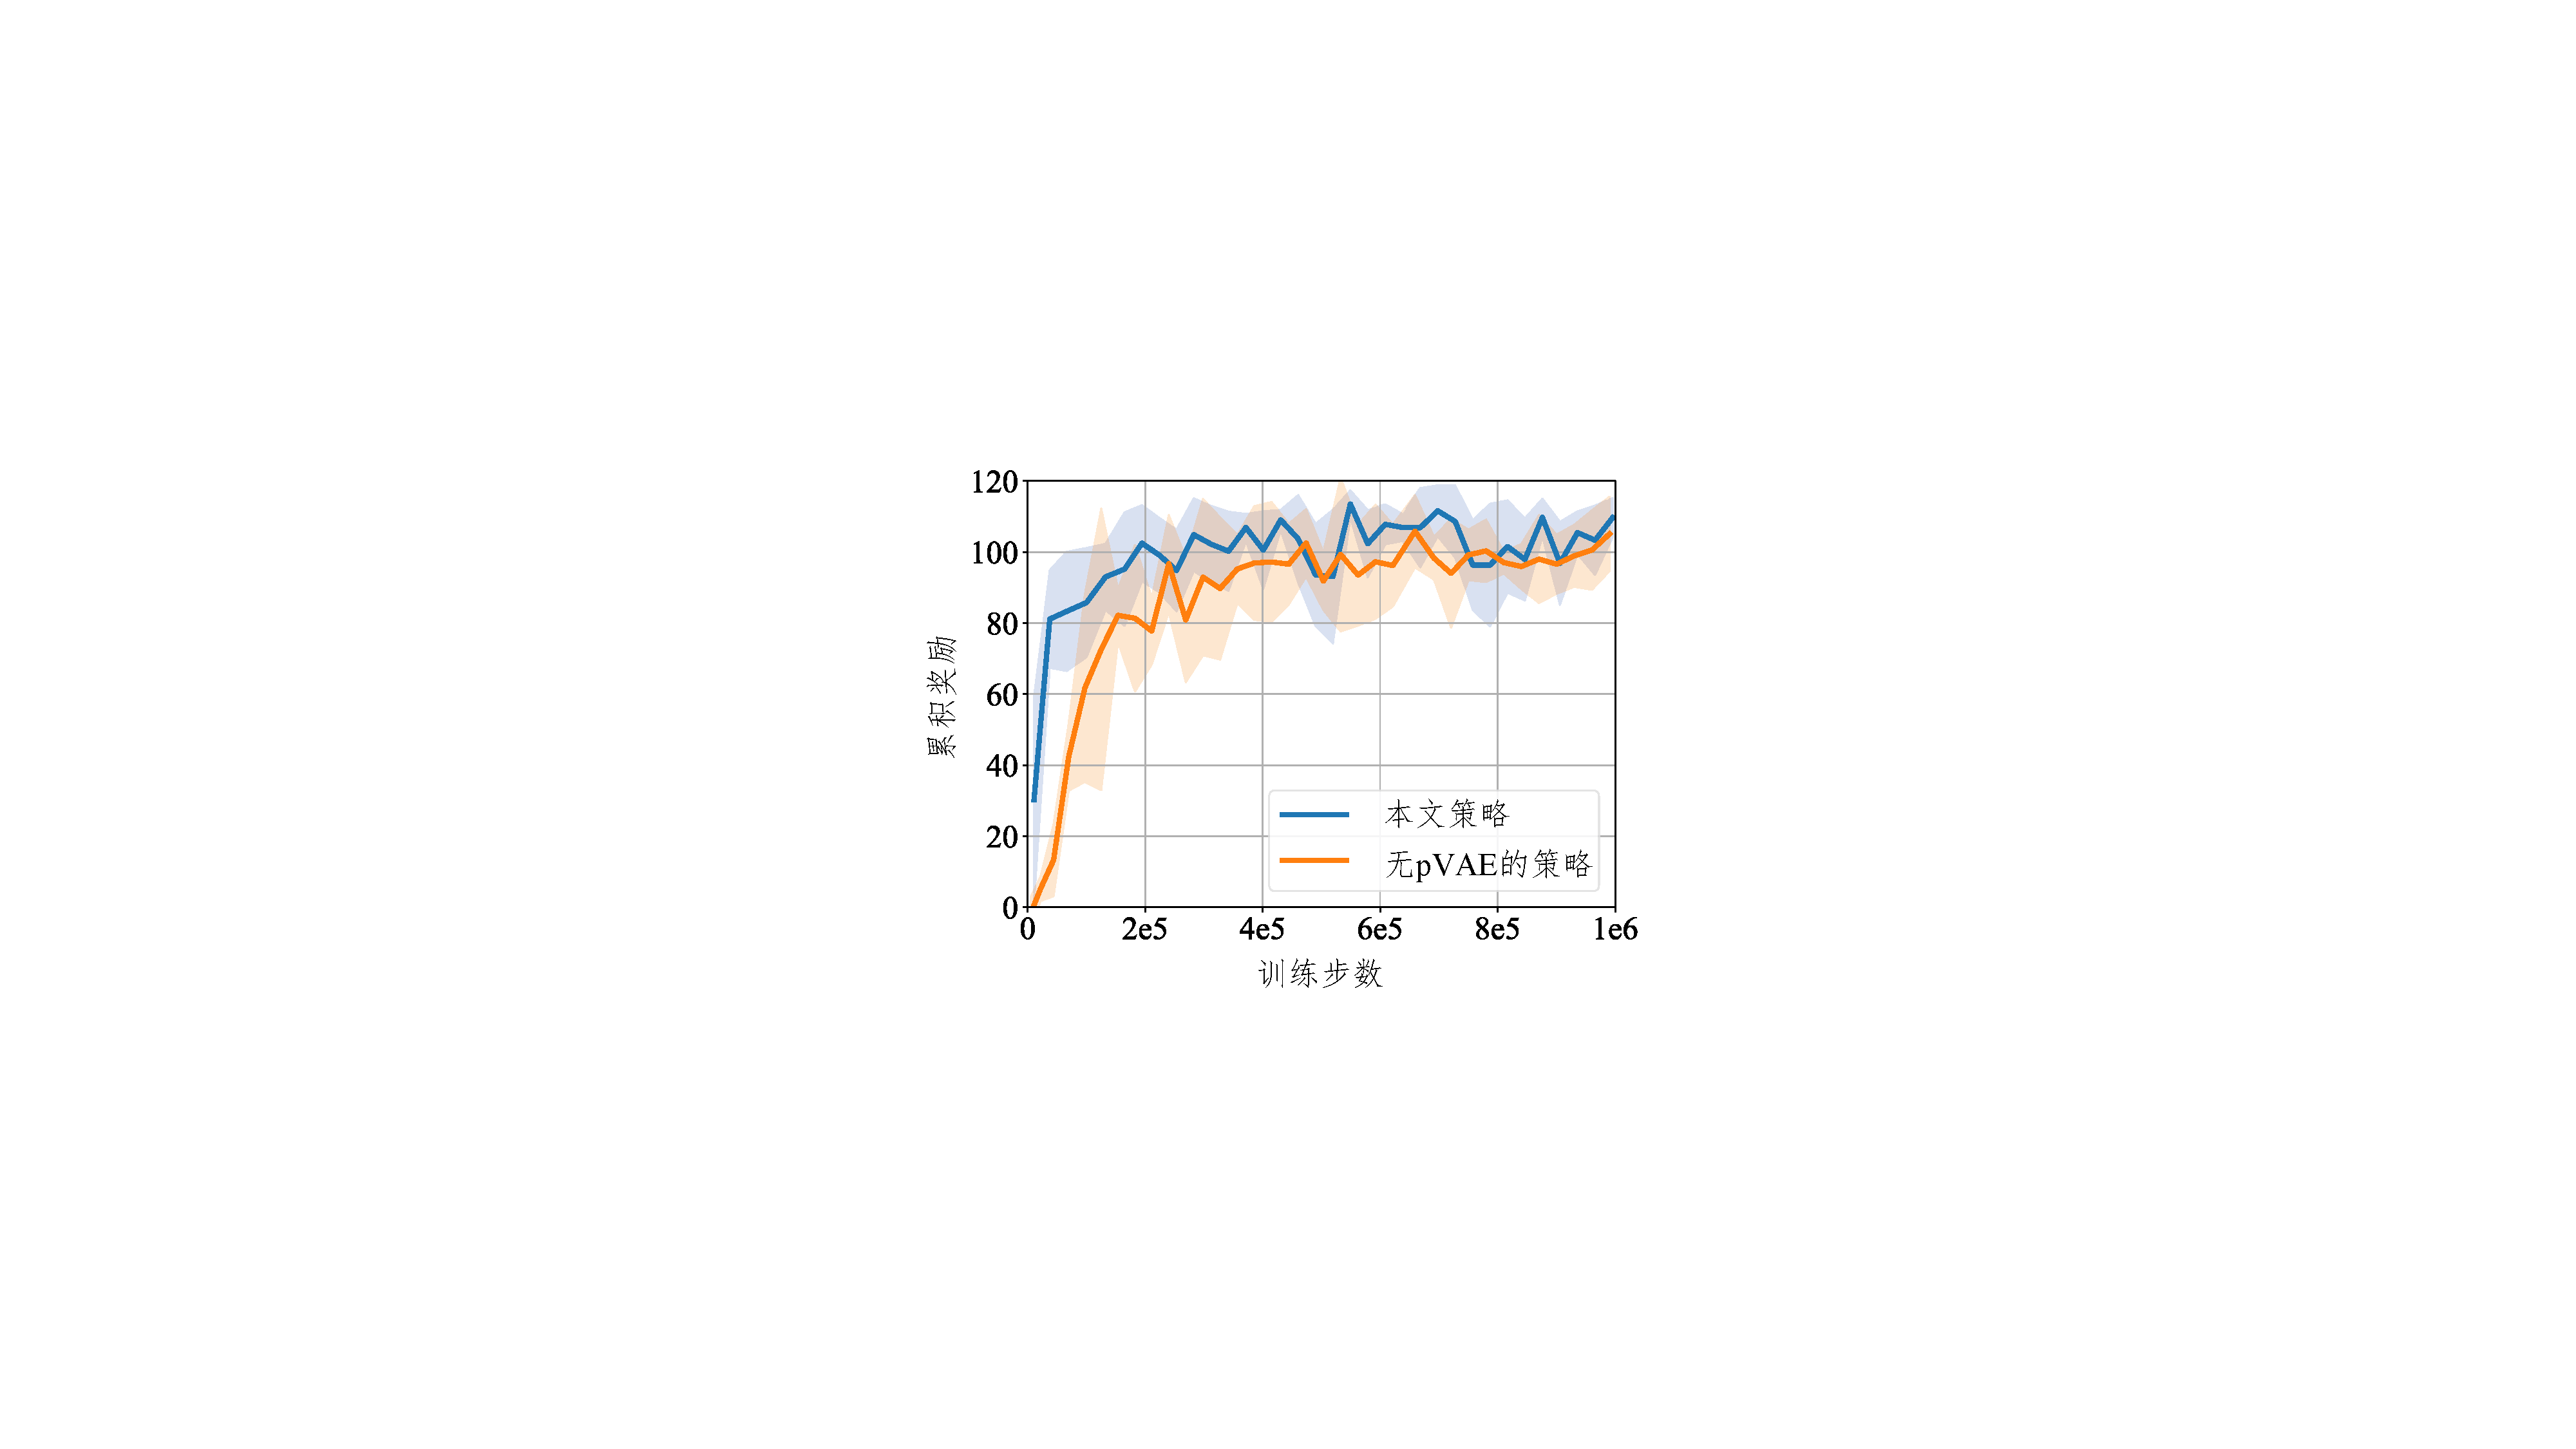
\includegraphics[width=0.45\linewidth]{figure/chapter3/vae-reward.pdf}}
    \subfloat[蒸馏损失]{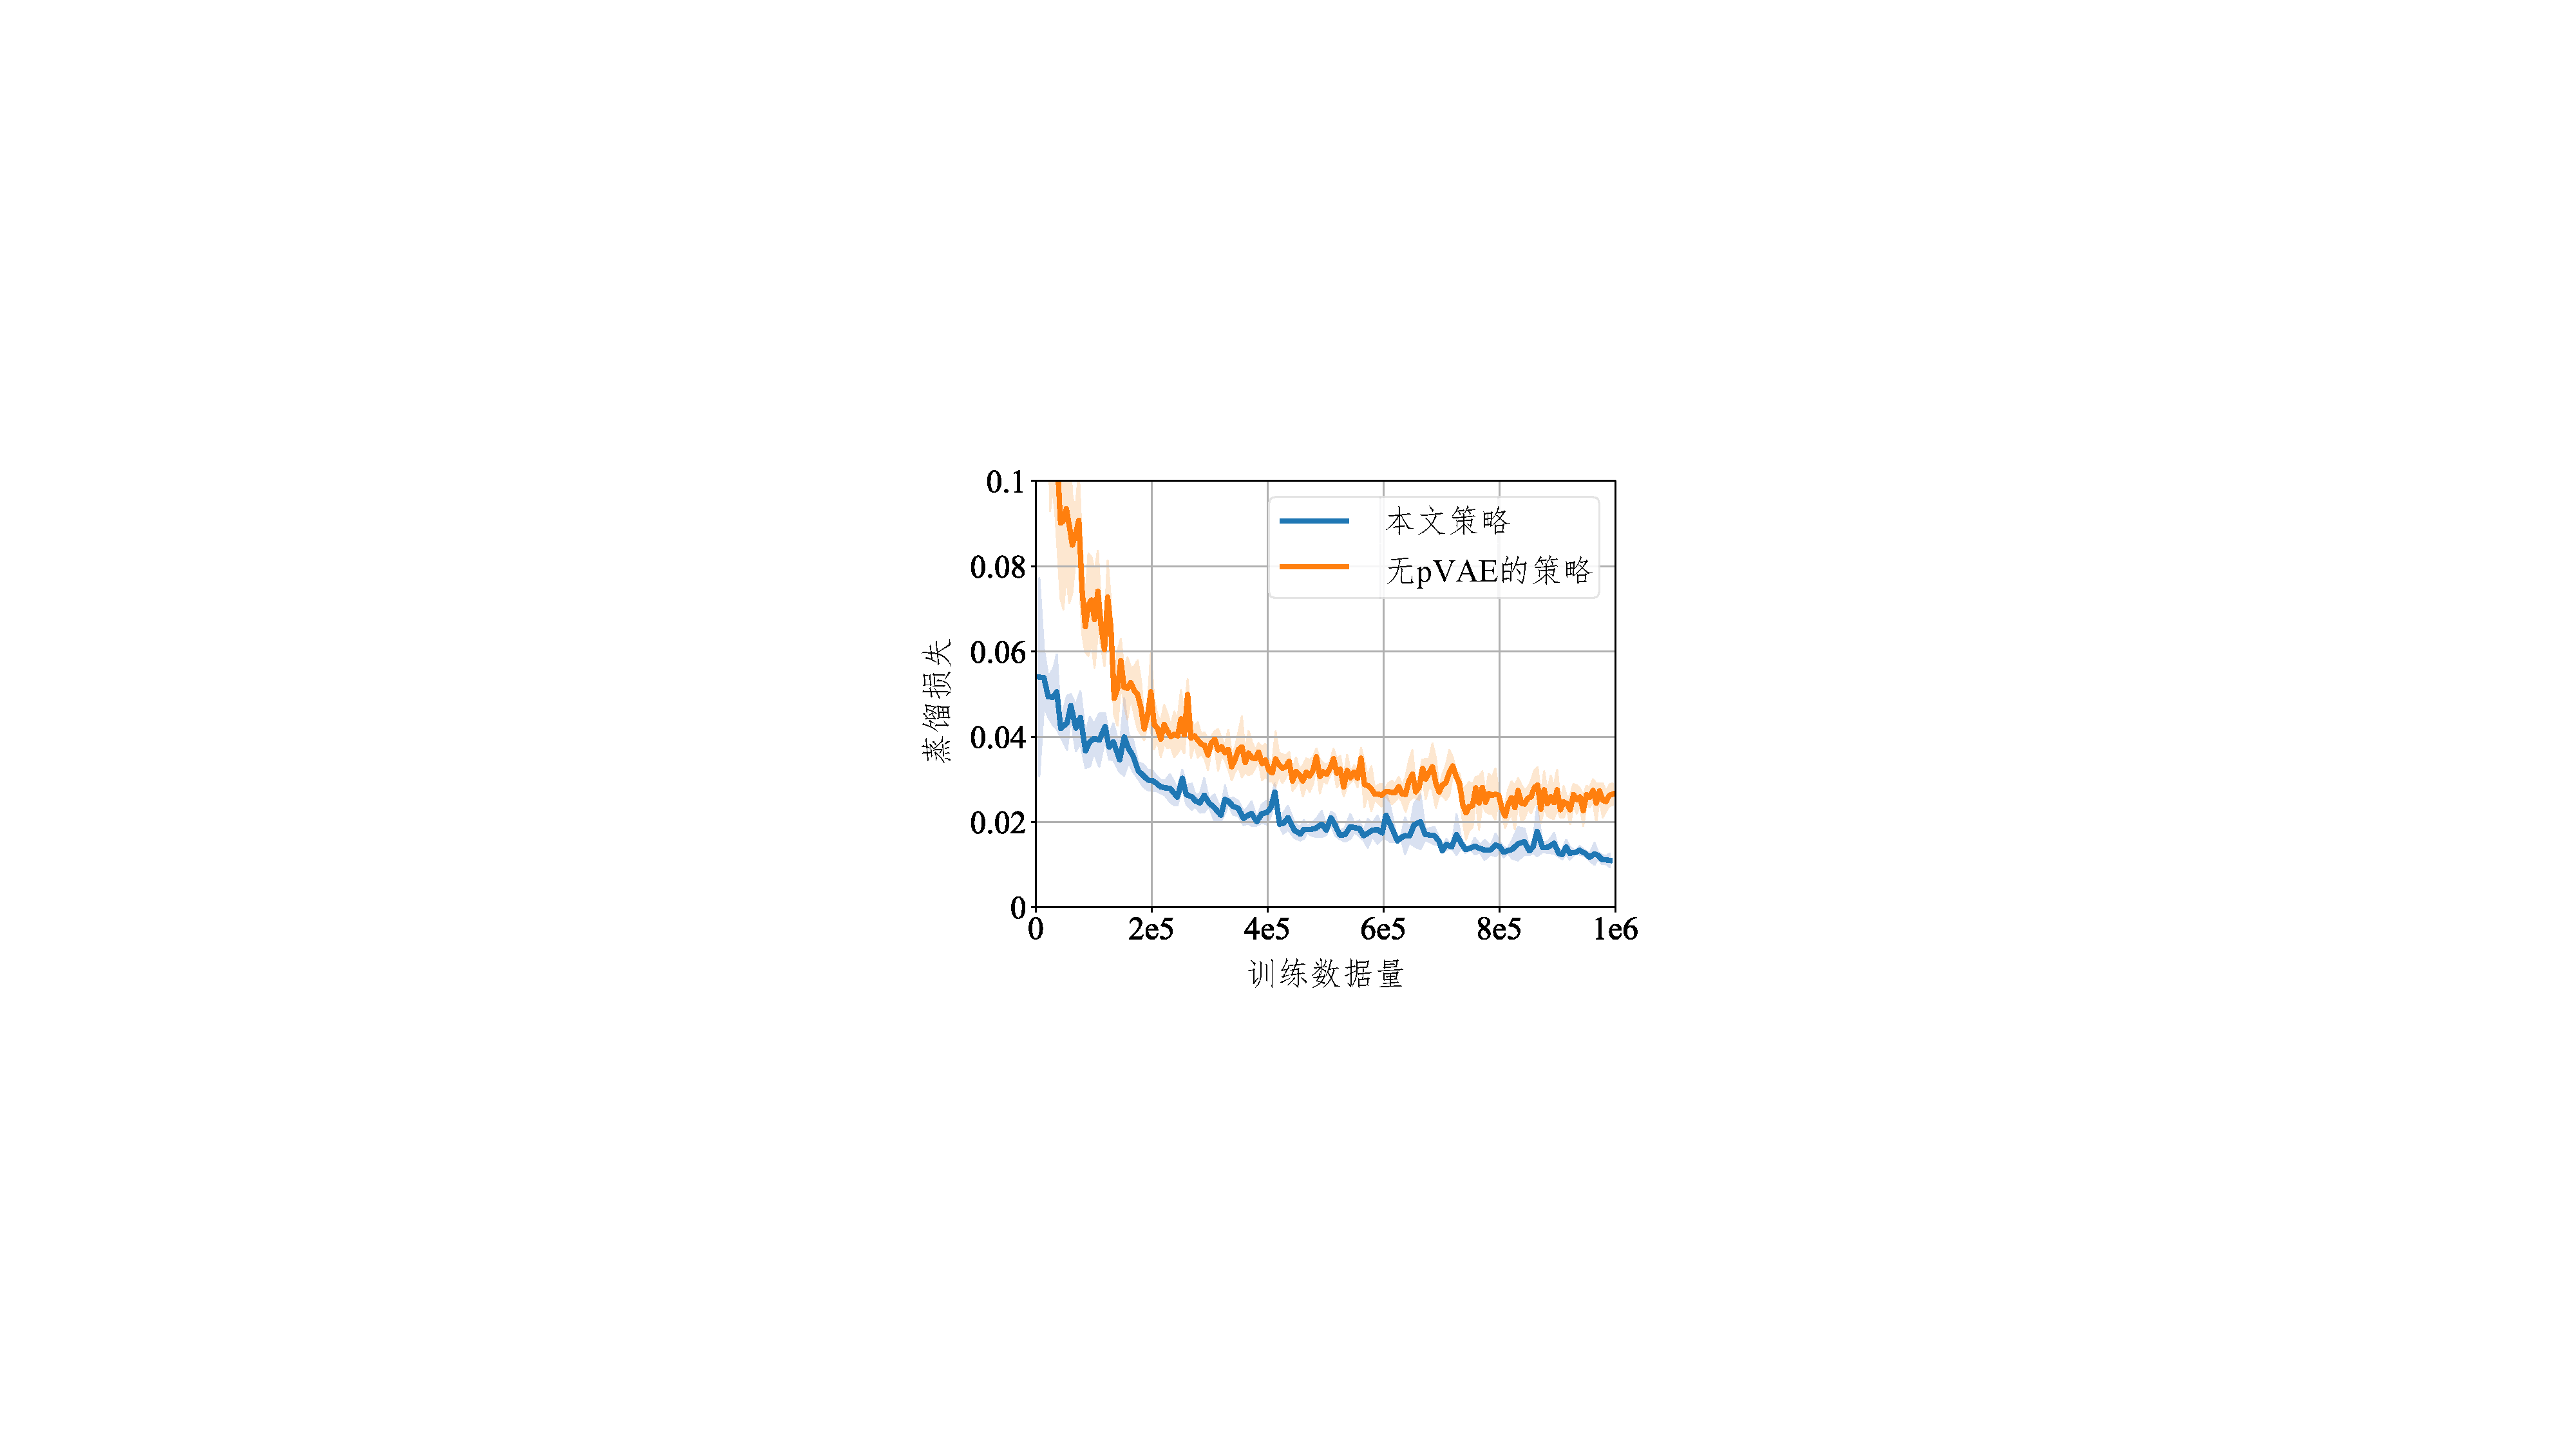
\includegraphics[width=0.45\linewidth]{figure/chapter3/vae-loss.pdf}}
    \caption{预训练VAE的消融实验}
    \label{fig:vae-ablation}
\end{figure}
\textbf{VAE预训练与潜在向量维度：}为了展现预训练VAE（简称pVAE）对学生策略的影响，我们将其与一个无预训练VAE的学生策略进行比较，该策略使用蒸馏损失端到端进行训练。两种策略拥有相同的视觉编码器结构，并由同一个教师策略进行蒸馏，训练过程中的累积奖励和蒸馏损失如图\ref{fig:vae-ablation}所示。由于预训练了视觉编码器，本文的学生策略在知识蒸馏的数据效率上存在较小的优势，两个策略在$6\times10^5$步训练后收敛到相似的累积奖励。然而，由于预训练的VAE对噪声存在鲁棒性，知识蒸馏的动作损失更低，在MCO赛道中测试时展现了更高的成功率和更低的平均跃度。因此，预训练的VAE更能有效提取视觉特征，有利于知识蒸馏并提高了策略的鲁棒性，我们在下一节的实物实验中进行了进一步验证。另外，本节还探索了VAE潜在向量维度的影响。当扩张维度至$N_z=128$时，编码器依旧能有效提取特征，竞速效果变化不大；当缩小维度至$N_z=32$时，编码器不能完整提取特征，竞速效果受到影响。

\begin{table}[ht]
\renewcommand{\arraystretch}{1.25}
\caption{在单一赛道训练的学生策略在不同赛道的测试结果}
\centering
\setlength{\tabcolsep}{8pt}{
    \begin{tabular}{c|ccc|ccc}
    \toprule[2pt]
        \multirow{3}{*}{\textbf{训练赛道}} & \multicolumn{3}{c|}{\textbf{测试赛道 AUT}} & \multicolumn{3}{c}{\textbf{测试赛道 ESP}}\\
        & 完成时间 & 平均跃度 & 成功率 & 完成时间 & 平均跃度 & 成功率 \\
        & [$s$] & [$m/s^3$] & [$\%$] & [$s$] & [$m/s^3$] & [$\%$] \\
    \midrule[1pt]
        AUT & 16.08$\pm$0.36 & 19.89$\pm$0.68 & 100 & 38.81$\pm$0.62 & 18.35$\pm$0.87 & 80.0 \\
        ESP & 16.84$\pm$0.55 & 24.04$\pm$1.12 & 60.0 & 37.18$\pm$0.32 & 16.83$\pm$0.53 & 100 \\
        GBR & 16.42$\pm$0.44 & 22.25$\pm$0.82 & 67.5 & 37.79$\pm$0.42 & 16.94$\pm$0.62 & 90.0 \\
        MCO & 16.24$\pm$0.41 & 21.87$\pm$0.70 & 77.5 & 37.81$\pm$0.49 & 17.15$\pm$0.57 & 92.5 \\
    \toprule[2pt]
        \multirow{3}{*}{\textbf{训练赛道}} & \multicolumn{3}{c|}{\textbf{测试赛道 GBR}} & \multicolumn{3}{c}{\textbf{测试赛道 MCO}}\\
        & 完成时间 & 平均跃度 & 成功率 & 完成时间 & 平均跃度 & 成功率 \\
        & [$s$] & [$m/s^3$] & [$\%$] & [$s$] & [$m/s^3$] & [$\%$] \\
    \midrule[1pt]
        AUT & 34.34$\pm$0.64 & 19.43$\pm$0.83 & 52.5 & 31.57$\pm$0.67 & 22.79$\pm$0.76 & 37.5 \\
        ESP & 33.65$\pm$0.53 & 18.27$\pm$0.64 & 70.0 & 30.64$\pm$0.47 & 21.64$\pm$0.58 & 62.5 \\
        GBR & 32.47$\pm$0.32 & 17.52$\pm$0.57 & 100 & 29.58$\pm$0.28 & 20.56$\pm$0.62 & 80.0 \\
        MCO & 32.64$\pm$0.36 & 17.68$\pm$0.65 & 95.0 & 29.35$\pm$0.24 & 19.87$\pm$0.53 & 100\\
    \bottomrule[2pt]
\end{tabular}}
\label{table:cross_validation}
\end{table}
\textbf{不同训练环境的泛化性：}本节进行了不同训练环境的交叉实验来展现策略的泛化性，教师策略和学生策略均只在一个赛道上进行训练，但在四个赛道中测试，测试结果如表\ref{table:cross_validation}所示。根据实验结果，我们可以发现所有策略都能在未知赛道中完成一圈竞速。当在训练赛道中竞速时，所有策略都表现最好；当在未知赛道竞速时，竞速表现有些许下滑，尤其是在简单赛道中训练的策略（例如AUT）。AUT赛道中训练的策略在位置赛道测试时会偶尔与赛道碰撞，导致了较低的成功率。然而，由于AUT赛道有一个有挑战性的急弯，在AUT赛道测试时依然是训练自AUT的策略表现最佳。相比较而言，在MCO赛道训练的策略泛化性最好，该策略在未知赛道中依然保持了高速运动策略与灵活避障性能，这归功于MCO赛道的复杂性和最多的弯道数量。

\subsection{仿真到实车迁移实验}
本节将学生策略部署到一辆1：10比例的赛车上来验证算法的可行性。赛车配有一个前视的双目深度相机，更新频率为30Hz；一个视觉里程计\cite{qin2018vins}也以30Hz的更新频率在线计算学生策略所需的运动状态估计；学生策略输出的指令由VESC电子调速器执行，其中加速度通过积分运算转换为电机的转速。图\ref{fig:real-sys}展示了本文的系统架构。
\begin{figure}[ht]
    \centering
    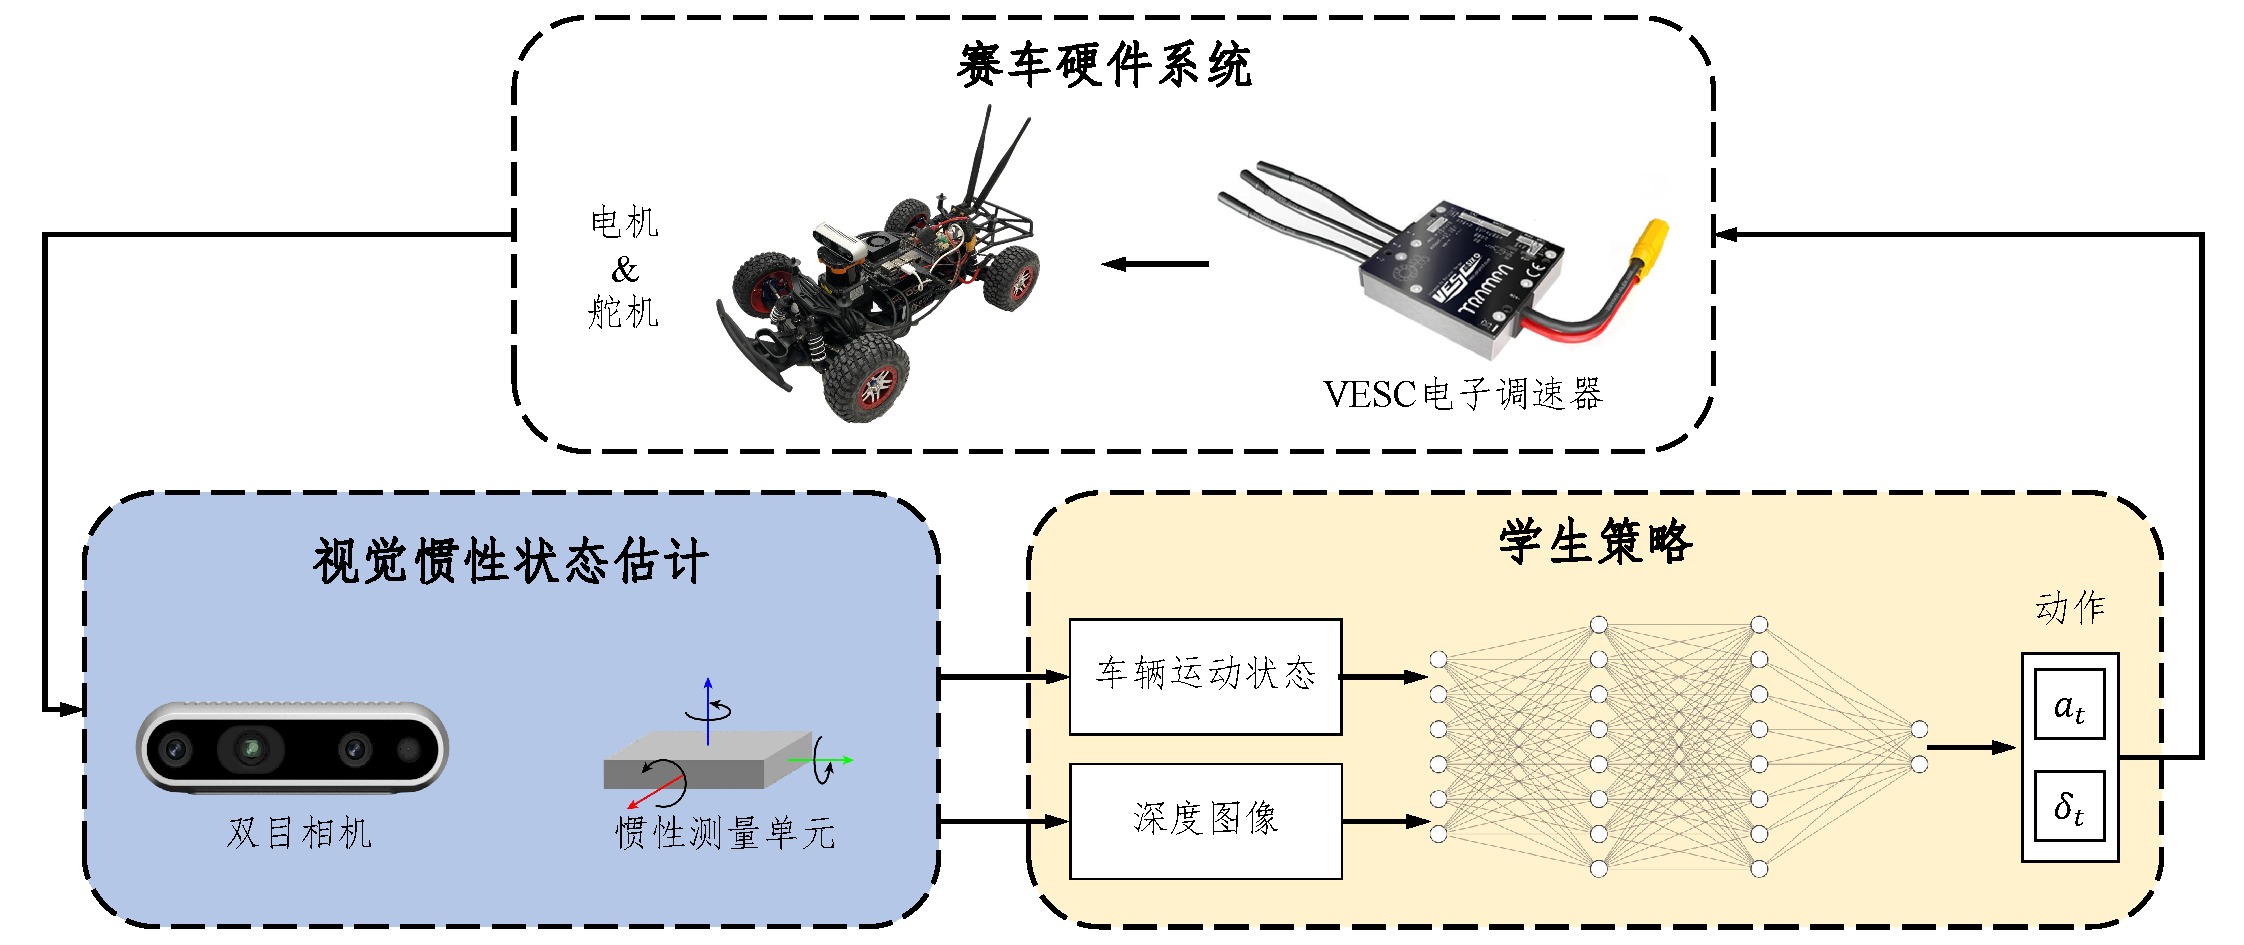
\includegraphics[width=0.9\linewidth]{figure/chapter3/real-sys.pdf}
    \caption{实车系统架构}
    \label{fig:real-sys}
\end{figure}

实验测试场地为一个$12m\times6m$的赛道，在训练过程中是不可见的。学生策略的竞速轨迹如图\ref{subfig:real-exp-map}所示，图中记录的数据由视觉里程计产生。本文提出的学生策略实现了零样本仿真-现实迁移，在图中赛道的完成时间为$9.62s$，最大速度为$5.58m/s$，最大加速度限制在$6m/s^2$。实物实验中产生的深度图像如图\ref{subfig:real-exp-depth}所示。VESC电子调速器接到的指令如图\ref{subfig:real-exp-prof}所示，可见控制指令的平滑性。
\begin{figure}[H]
    \centering
    \subfloat[竞速轨迹]{\label{subfig:real-exp-map}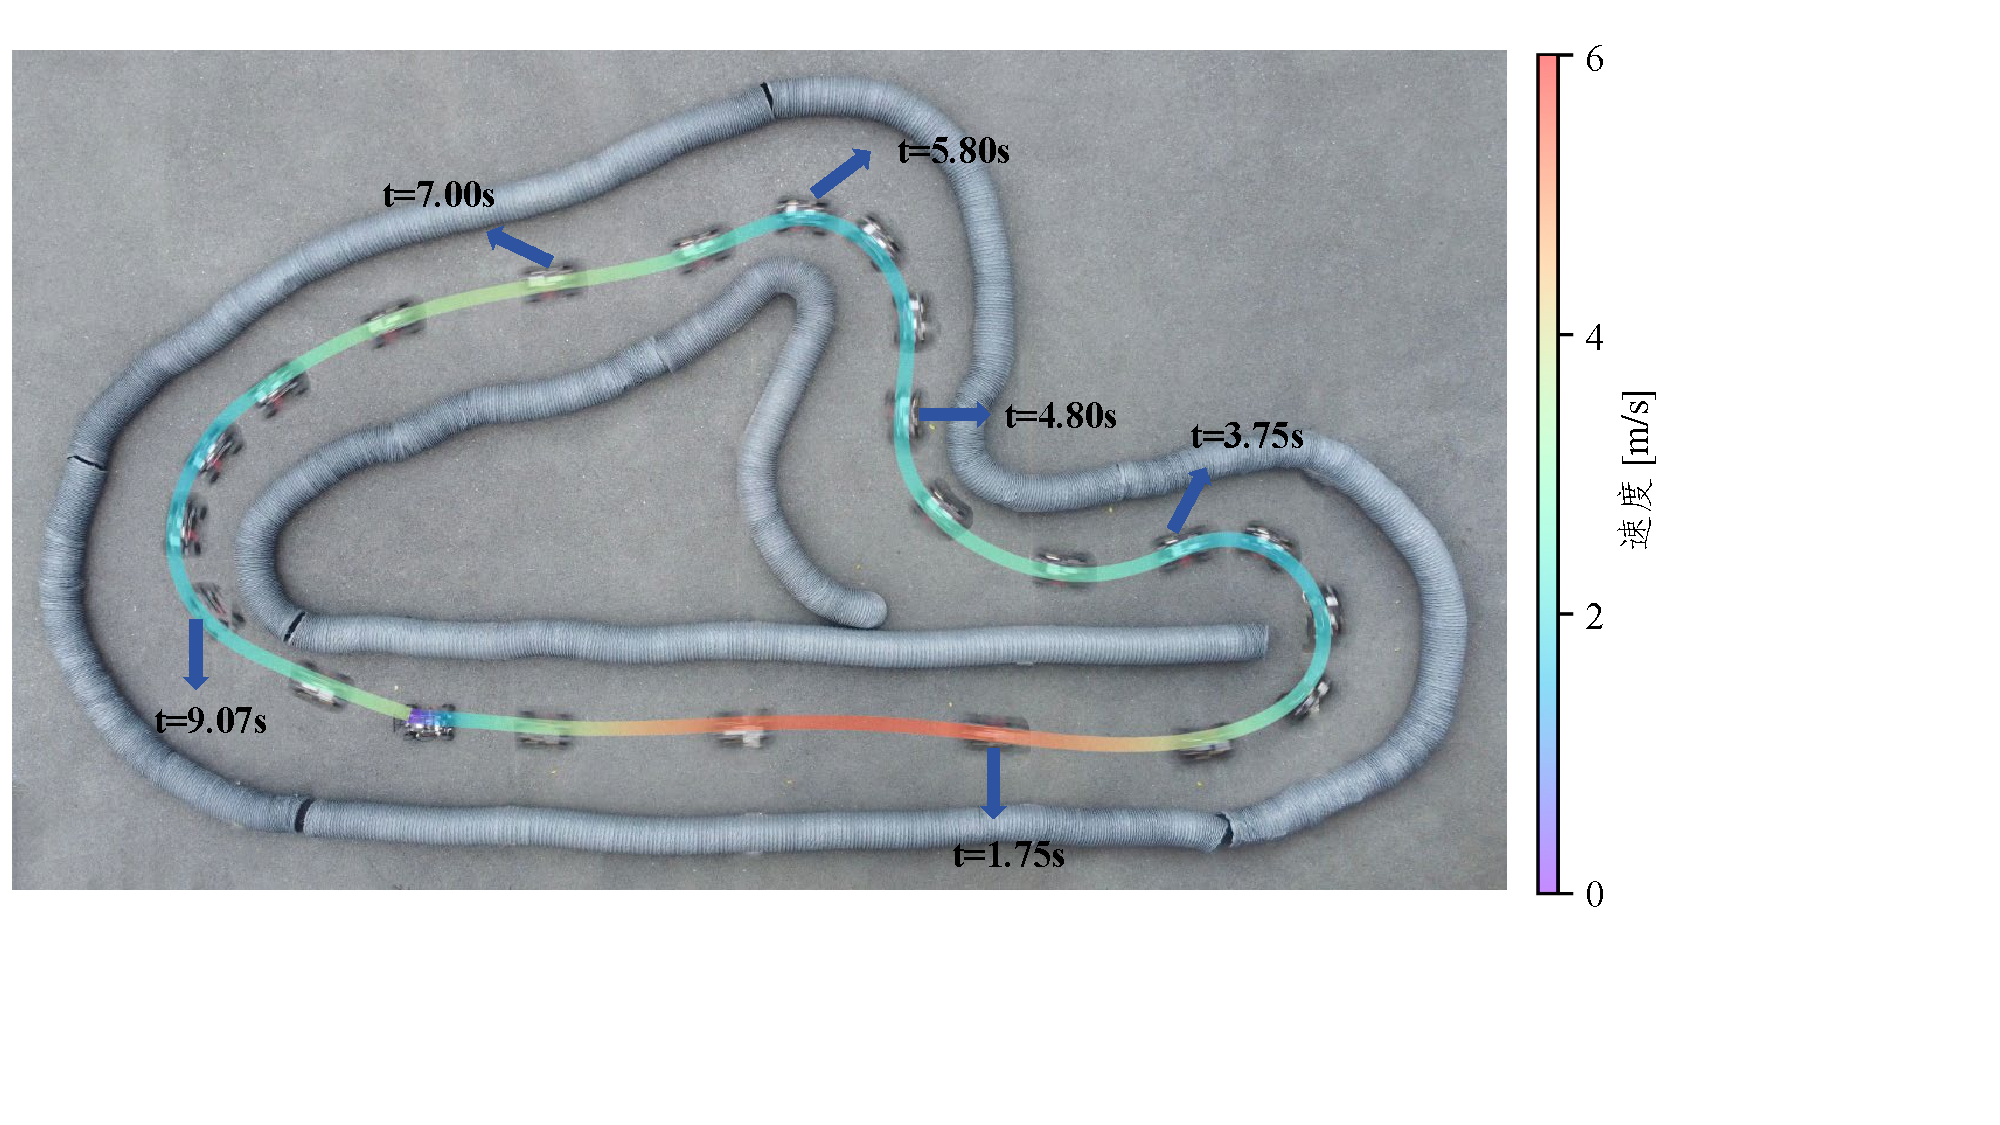
\includegraphics[width=0.75\linewidth]{figure/chapter3/real_exp_map.pdf}}

    \subfloat[深度图像]{\label{subfig:real-exp-depth}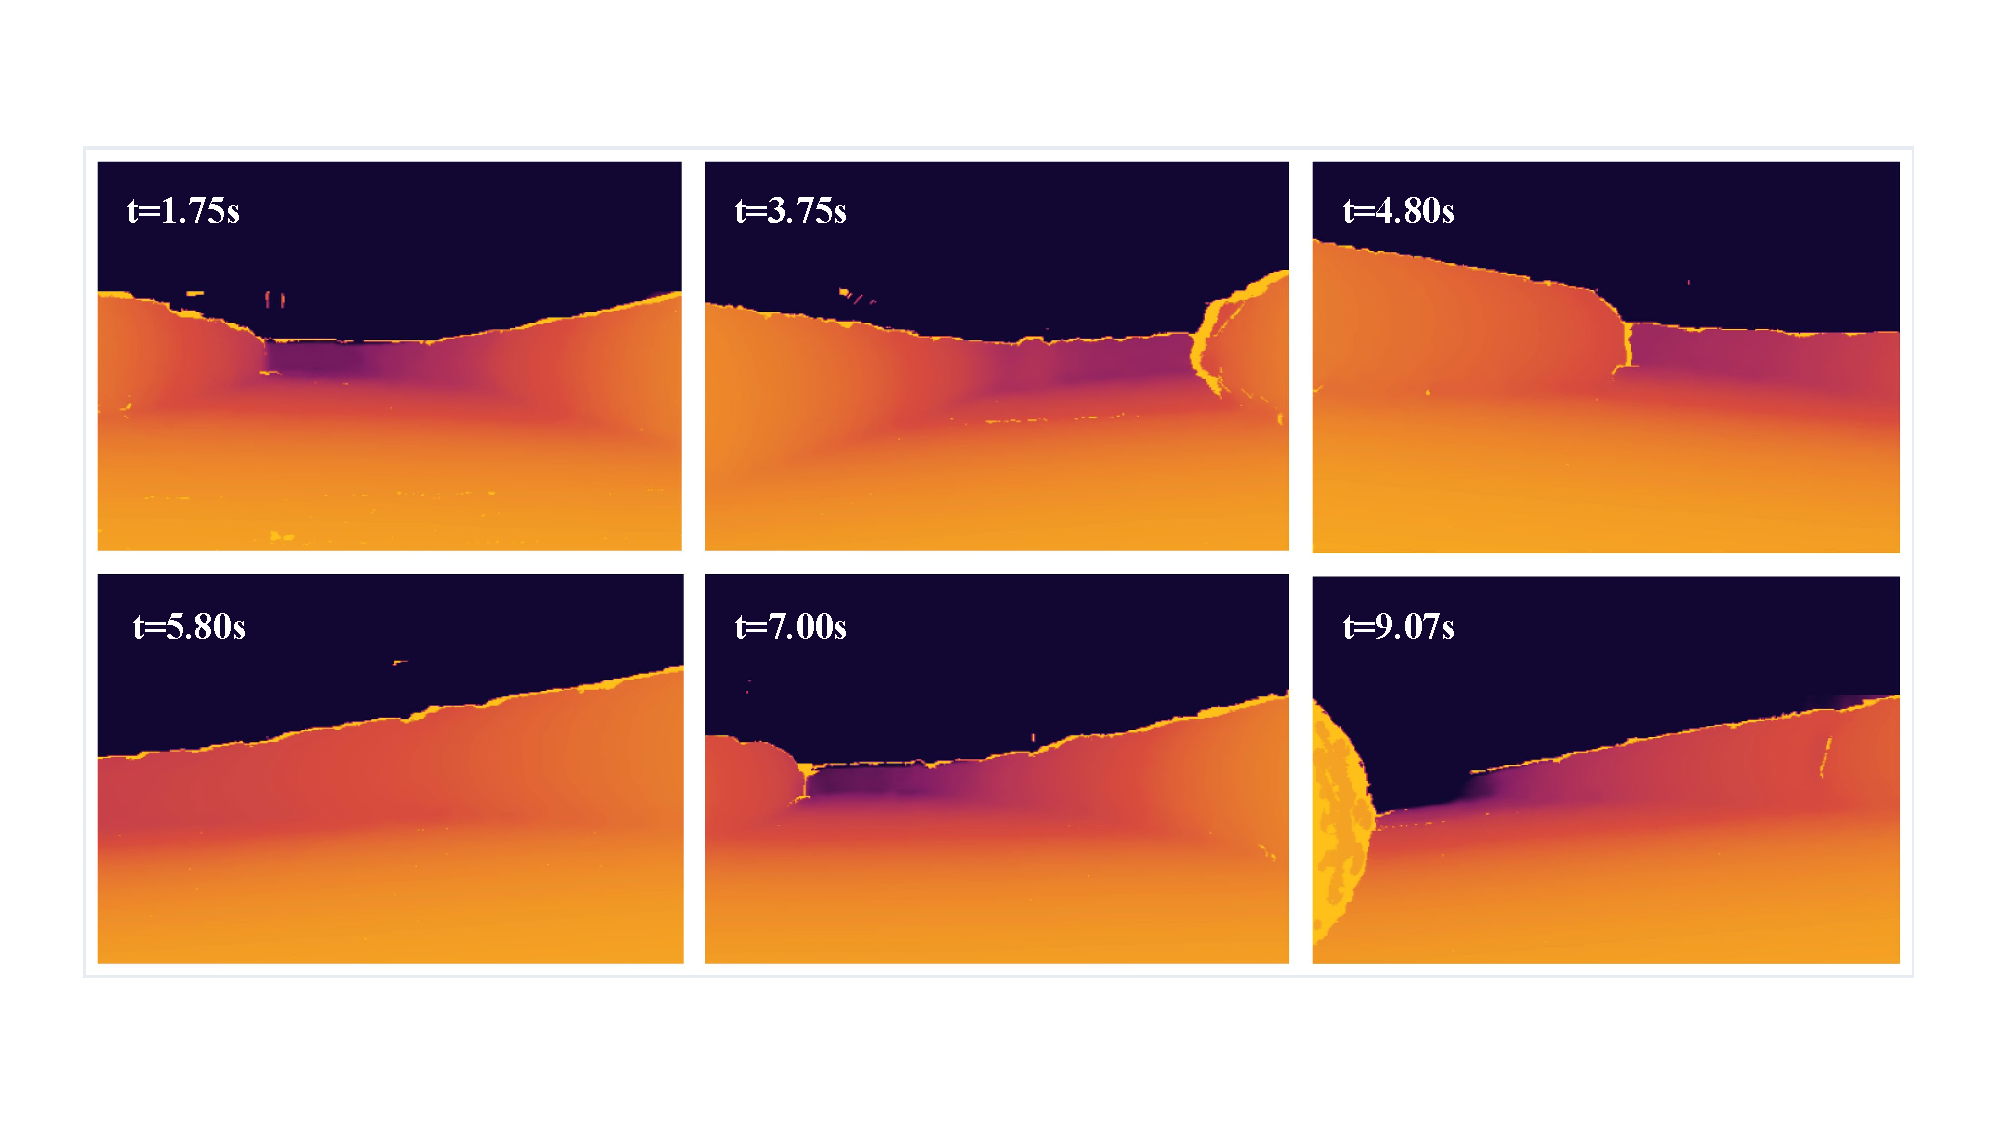
\includegraphics[width=0.75\linewidth]{figure/chapter3/real_exp_depth.pdf}}

    \subfloat[控制量变化曲线]{\label{subfig:real-exp-prof}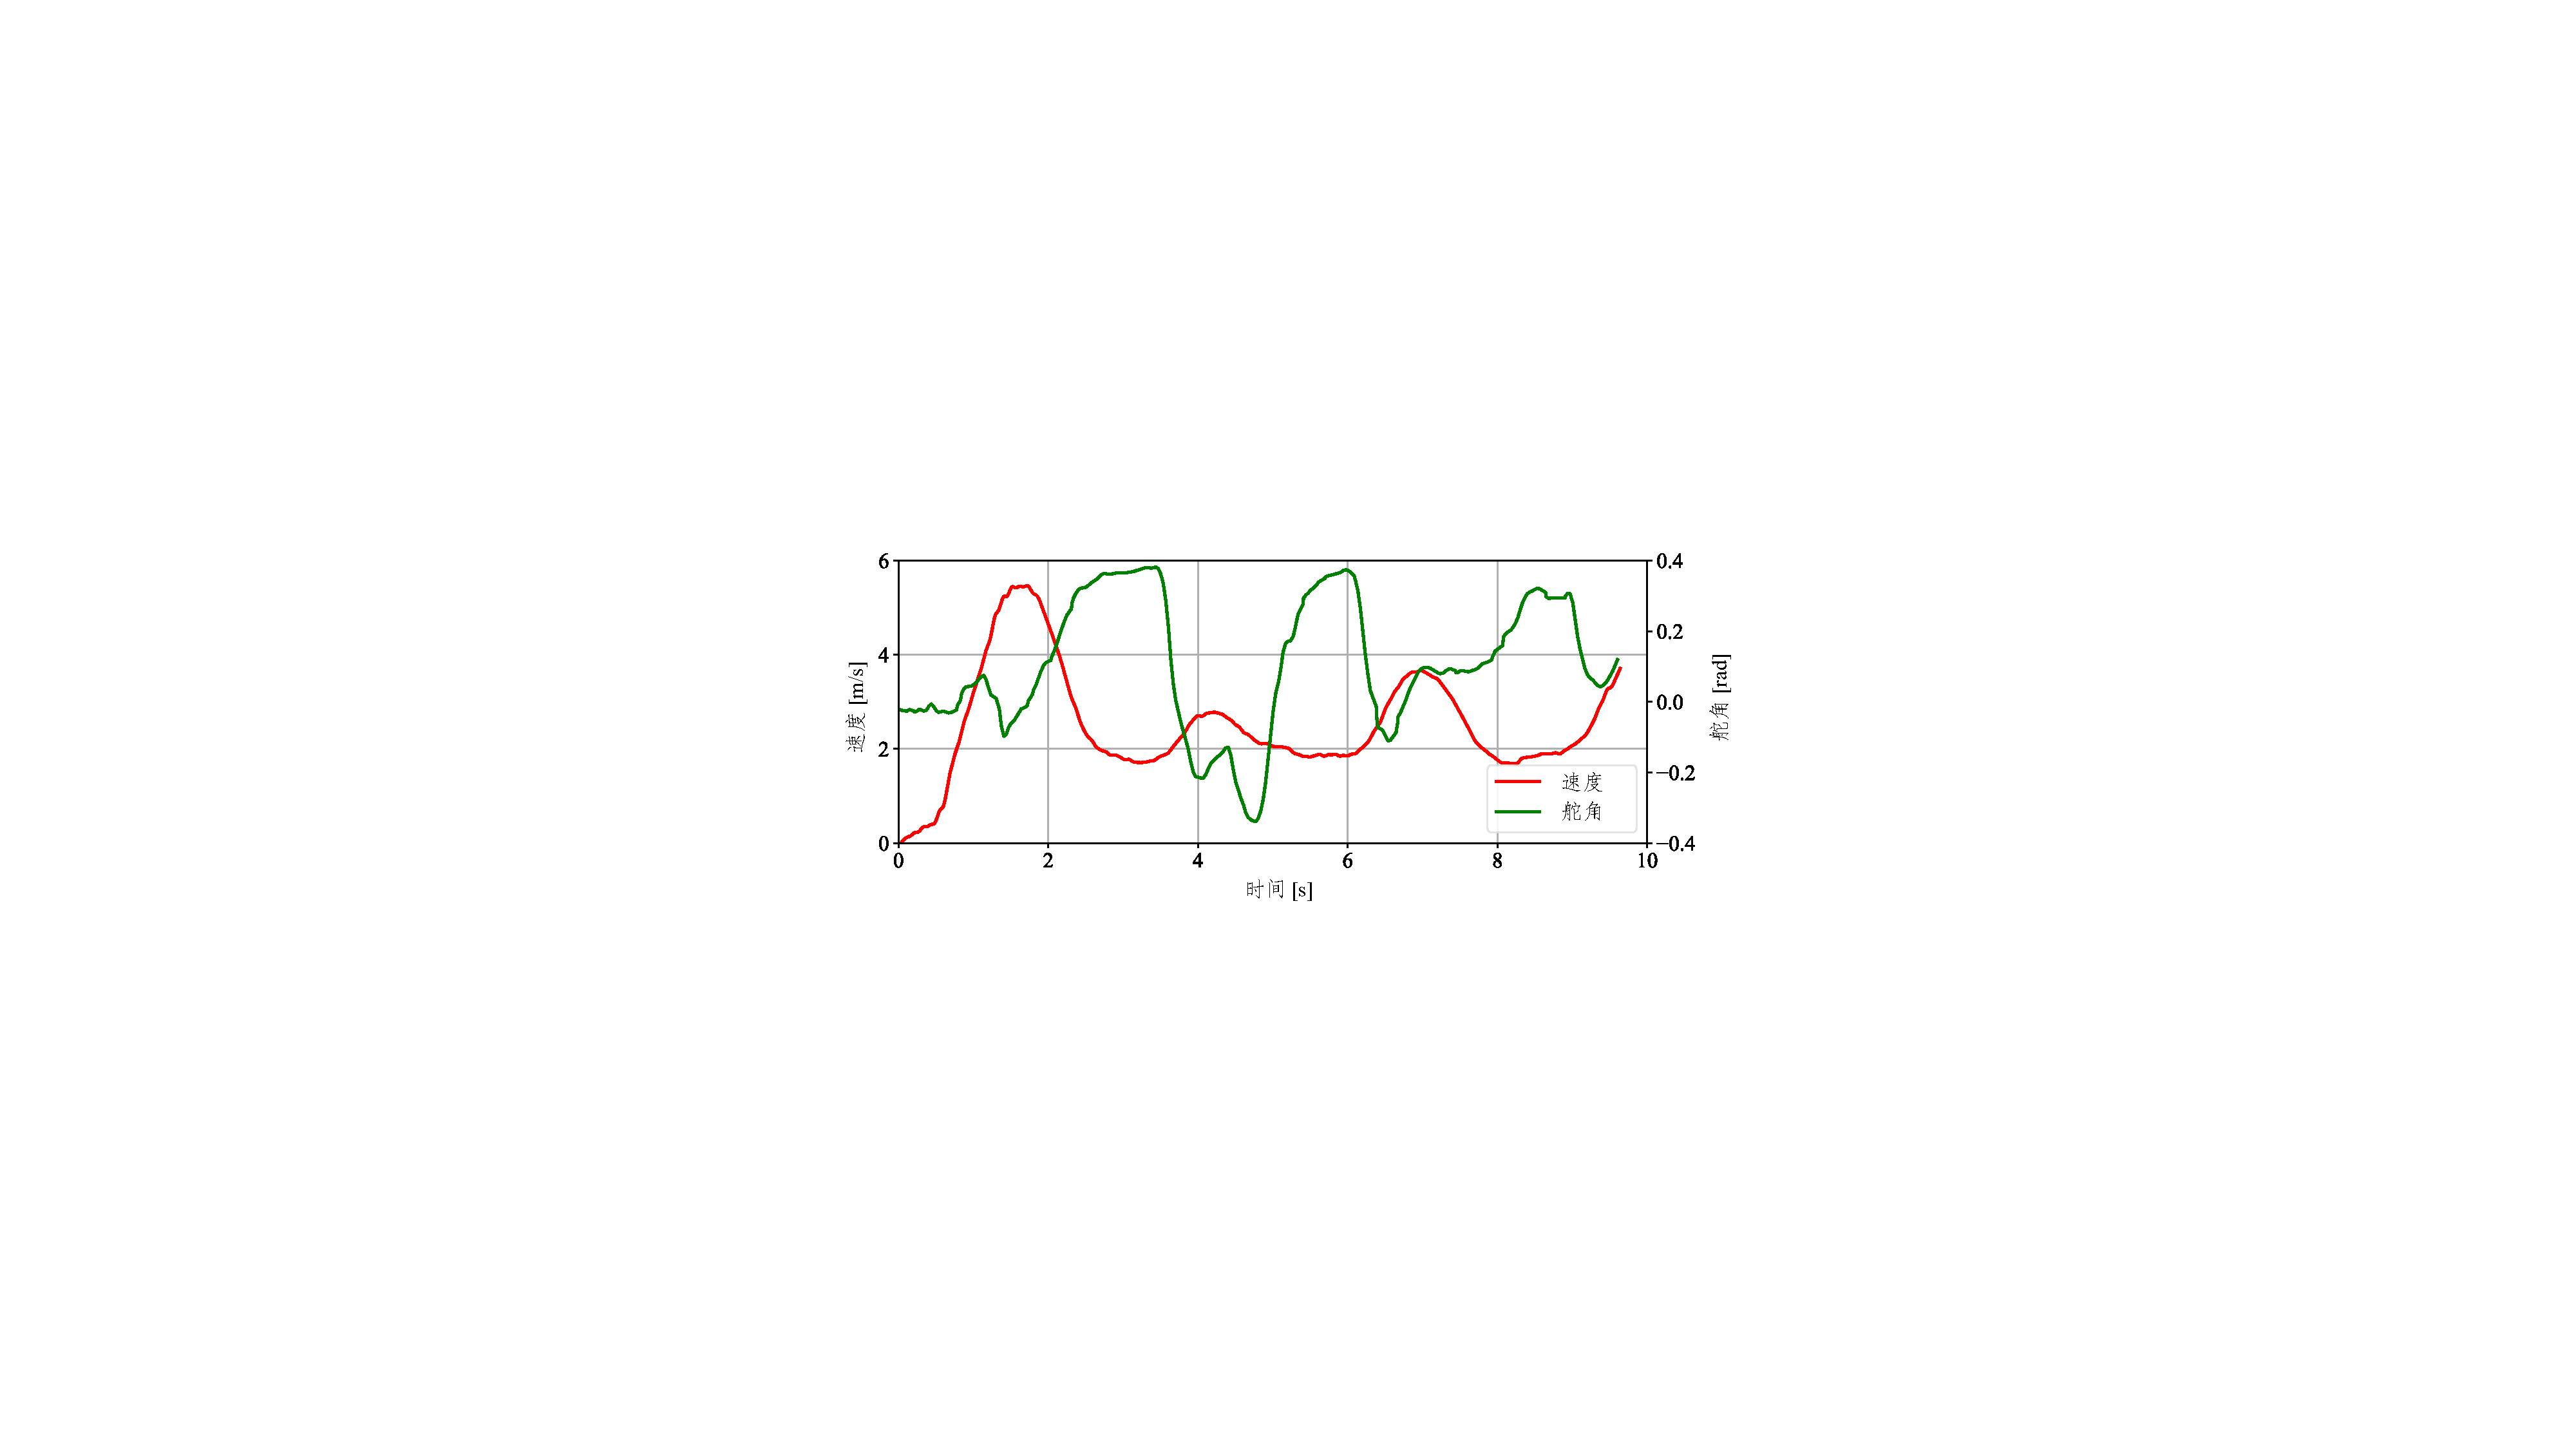
\includegraphics[width=0.75\linewidth]{figure/chapter3/real_exp_prof.pdf}}
    \caption{实车实验}
    \label{fig:real-exp}
\end{figure}

为了展示本文方法对不同路面情况的泛化性，我们在图\ref{fig:real-track}中所示的两个赛道上铺设了两种路面进行实验：沥青路面和橡胶路面，测试结果如表\ref{table:real_texture}所示。在无微调的前提下，本文的方法可以在两个赛道、两个路面的环境中完成竞速测试。由于橡胶路面比沥青路面的摩擦系数更低，赛车在橡胶路面上进弯道时容易发生漂移现象，弯道的竞速轨迹因此有时靠近赛道外侧，导致了较长的完成时间。在橡胶路面上的漂移在少数情况下也会引起不安全的竞速行为。
\begin{figure}[ht]
    \centering
    \subfloat[赛道1（$7m\times4m$）]{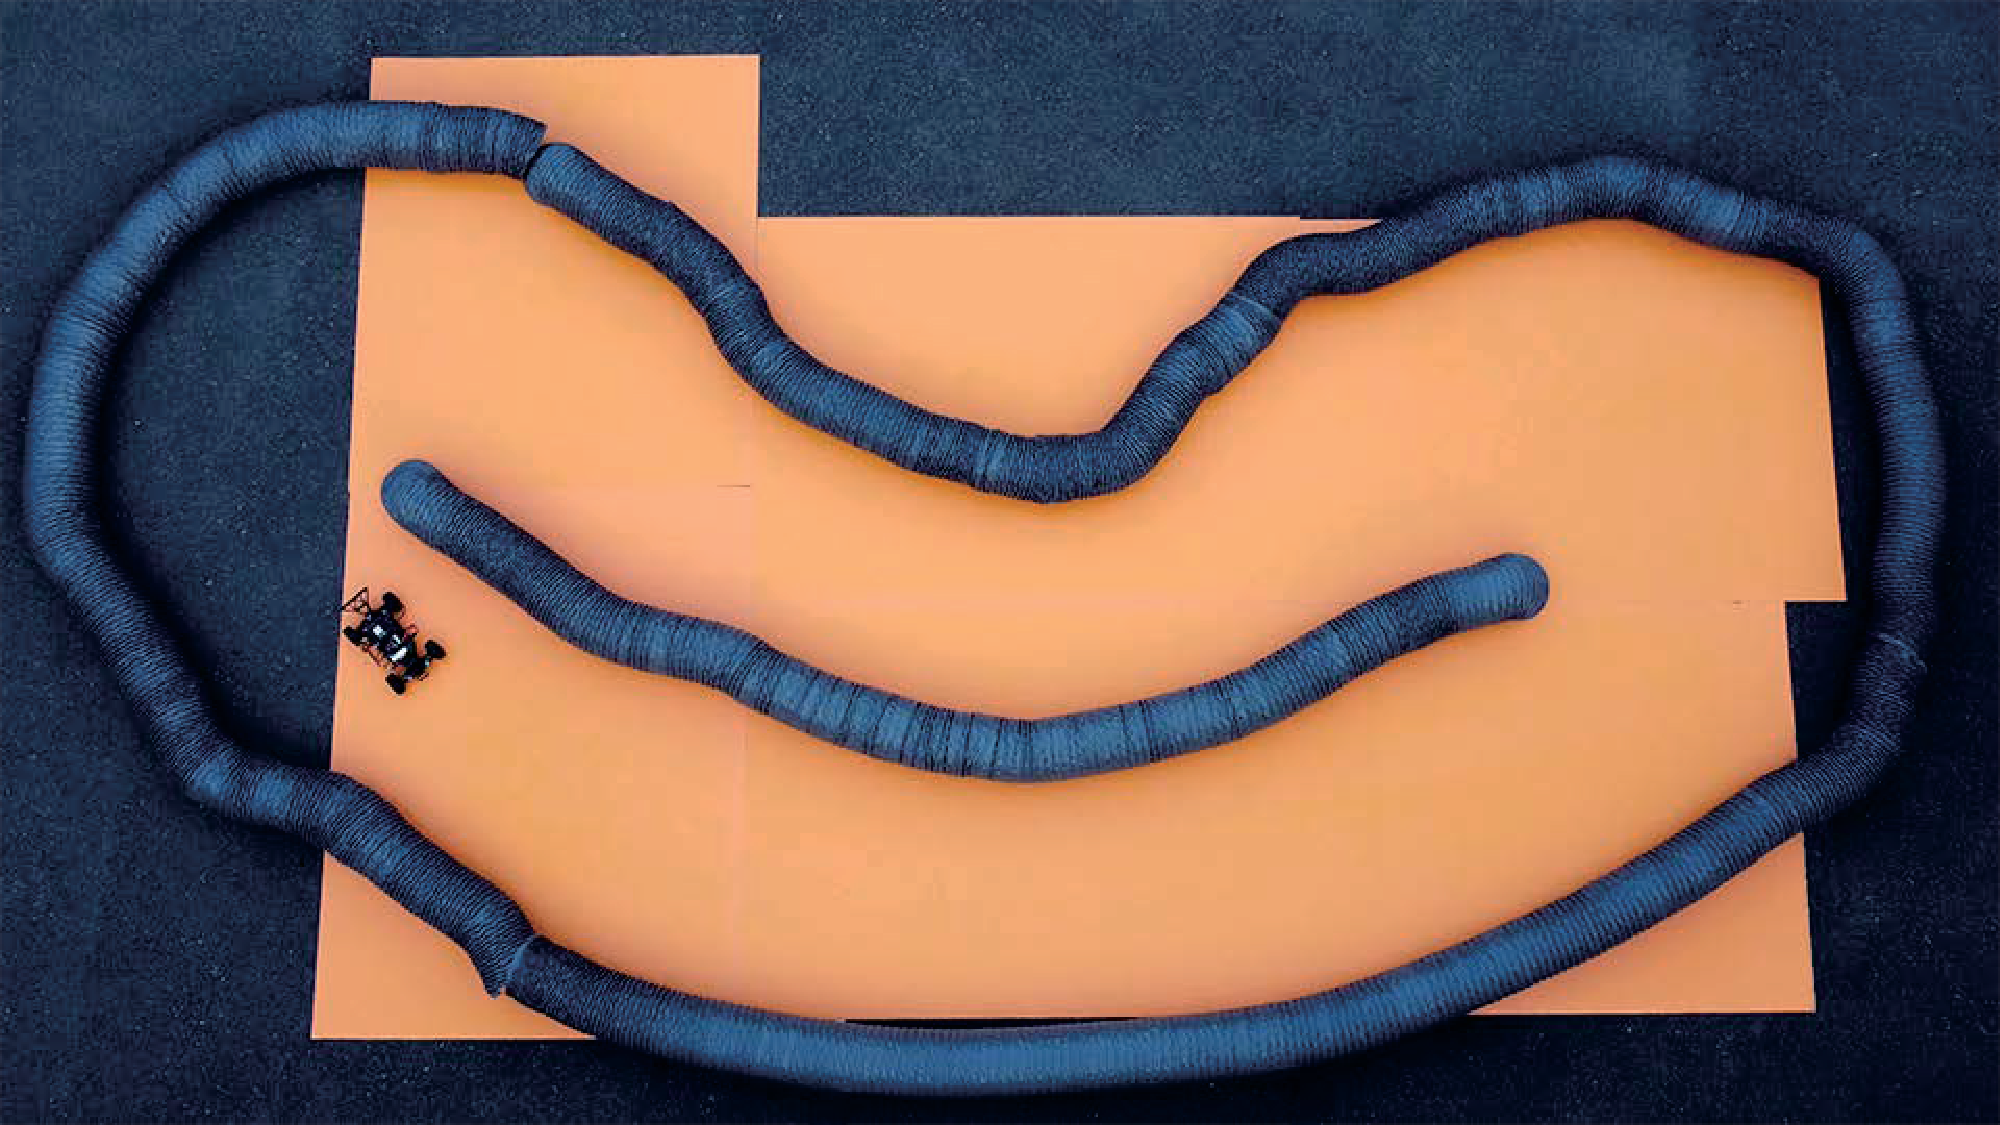
\includegraphics[width=0.5\linewidth]{figure/chapter3/racetrack1.pdf}}
    \subfloat[赛道2（$8m\times6m$）]{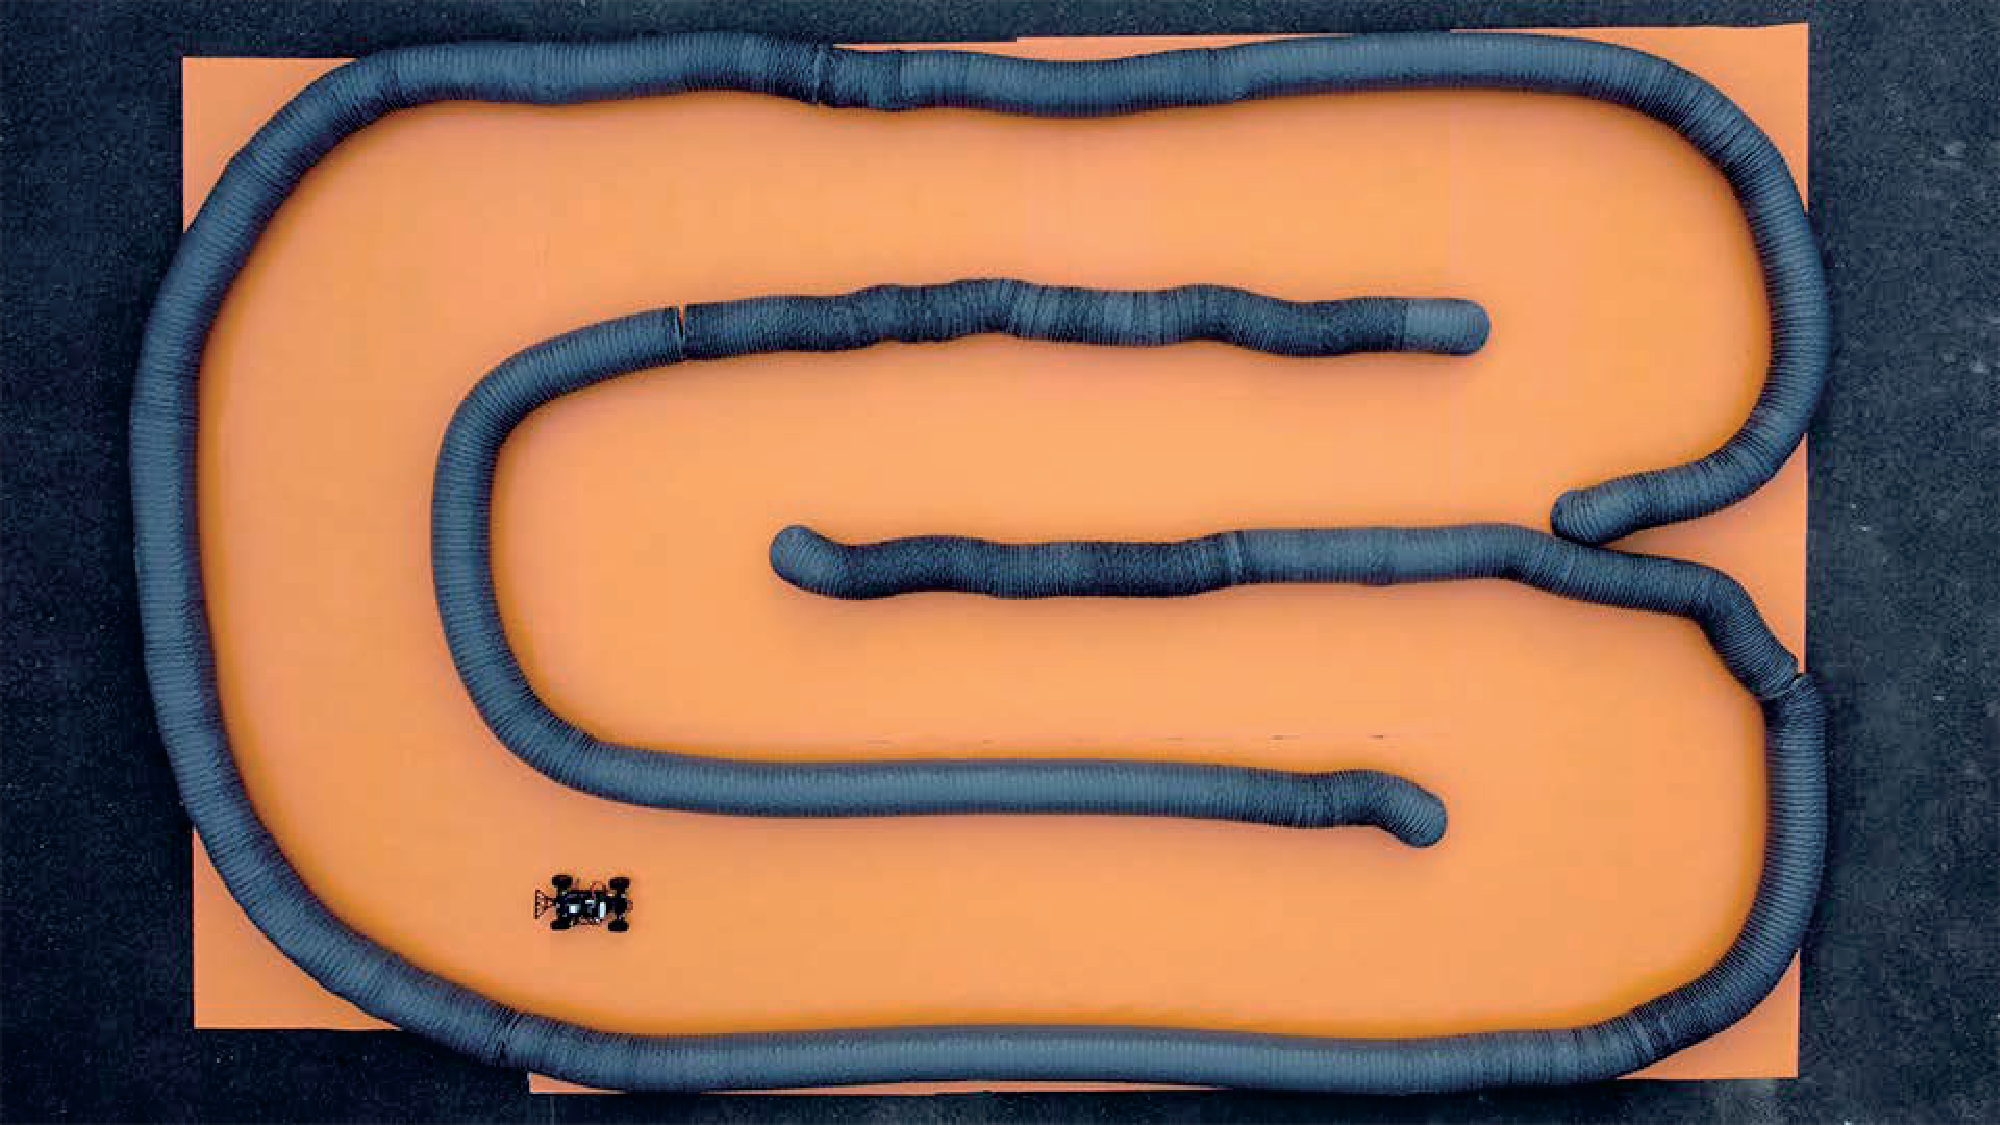
\includegraphics[width=0.5\linewidth]{figure/chapter3/racetrack2.pdf}}
    \caption{实车实验所用到的赛道}
    \label{fig:real-track}
\end{figure}
\begin{table}[ht]
\renewcommand{\arraystretch}{1.25}
\caption{在不同路面下学生策略的测试结果}
\centering
\setlength{\tabcolsep}{12pt}{
    \begin{tabular}{c|c|cccc}
    \toprule[2pt]
        \multirow{2}{*}{\textbf{赛道}} & \multirow{2}{*}{\textbf{路面材质}} & 是否完成 & 完成时间 & 最大速度 & 平均速度\\
        & & [\cmark or \xmark] & [$s$] & [$m/s$] & [$m/s$]\\
    \midrule[1pt]
        \multirow{2}{*}{1}& 沥青 & \cmark & 6.96 & 4.37 & 2.81\\
        & 橡胶 & \cmark & 7.23 & 4.26 & 2.76\\
    \midrule[1pt]
        \multirow{2}{*}{2}& 沥青 & \cmark & 13.17 & 4.69 & 2.44\\
        & 橡胶 & \cmark & 14.38 & 4.29 & 2.22\\
    \bottomrule[2pt]
\end{tabular}}
\label{table:real_texture}
\end{table}

\begin{table}[H]
\renewcommand{\arraystretch}{1.25}
\caption{不同控制策略在实物实验中的竞速效果比较}
\centering
\setlength{\tabcolsep}{12pt}{
    \begin{tabular}{c|c|cccc}
    \toprule[2pt]
        \multirow{2}{*}{\textbf{赛道}} & \multirow{2}{*}{\textbf{控制策略}} & 是否完成 & 完成时间 & 最大速度 & 平均速度 \\
        & & [\cmark or \xmark] & [$s$] & [$m/s$] & [$m/s$]\\
    \midrule[1pt]
        \multirow{4}{*}{1} & TAL & \cmark & 9.04 & 3.59 & 2.47 \\
        & 本文策略 & \cmark & 6.96 & 4.37 & 2.81 \\
        & 无GRU策略 & \xmark & - & 5.17 & 3.17 \\
        & 无pVAE策略 & \cmark & 7.17 & 4.57 & 2.74 \\
    \midrule[1pt]
        \multirow{4}{*}{2} &TAL & \cmark & 17.74 & 3.64 & 2.17 \\
        & 本文策略 & \cmark & 13.17 & 4.69 & 2.44 \\
        & 无GRU策略 & \xmark & - & 5.34 & 3.43 \\
        & 无pVAE策略 & \xmark & - & 5.59 & 3.49 \\
    \bottomrule[2pt]
\end{tabular}}
\label{table:real_policy}
\end{table}

另外，本文还在实物实验中比较了不同方法的竞速效果，实验结果如表\ref{table:real_policy}所示。无GRU结构的学生策略展现了最差的泛化性，无法在赛道中完成竞速。无预训练VAE的学生策略可以在赛道1中完成赛道，且与本文学生策略完成时间相近，但在赛道2中表现不佳，经常与赛道边界碰撞。这两者与本文策略的比较进一步说明了GRU结构对于部分可观决策任务的重要性，以及预训练VAE对控制策略鲁棒性的提升。本文的学生策略和TAL策略都实现了较好的泛化性，但和仿真结果类似，TAL的竞速性能较差，完成时间超过本文的学生策略。
\section{本章小结}
本章提出了一种两阶段的数据驱动的方法来训练自动驾驶赛车的端到端控制策略。在本章提出的方法中，强化学习算法利用仿真中的特权信息训练了一个教师策略；随后知识蒸馏算法将教师策略中的最优控制策略蒸馏至一个基于视觉的学生策略中。在学生策略中，本章设计了一个CNN-GRU-MLP网络结构处理视觉时序信息，并由VAE预训练视觉编码器实现鲁棒的特征提取。与基于模型的方法和基于学习的其他方法相比，本文提出的方法在四个维度上展现出优势：完成时间、成功率、平均跃度和数据效率。本章还进行了消融实验来评估重要组件对竞速效果的影响。最后，学生策略在实物实验中验证了有效性、泛化性，实现了零样本的仿真-现实迁移。
